\section{Introduction}

Topology optimization (TO) is an advanced computer-based design method used for creating efficient topologies via a reasonable material distribution satisfying performance requirements and constraints. Domains such as aerospace \parencite{zhu2016topology}, automotive \parencite{jankovics2019customization}, civil engineering \parencite{jewett2019topology} and mechanical engineering \parencite{guanghui2020aerospace, ZHU202191} use this sub-field of engineering proactively to create high-performance, lightweight and innovative design solutions that will outperform manual designs. TO algorithms are capable of creating sustainable designs while still being rooted in sound logic. Also, topologically optimized products save resources through weight reduction, by minimizing material usage. A great example is how General Electric used TO to reduce the weight of an engine bracket by 84\%, as shown in Figure \ref{fig:MDP_Fig1_mounted_bracket}. This modification in a small part saved the airlines nearly 31 million dollars by improving the overall energy efficiency \parencite{morgan2014ge}. Another useful example of a TO solution is the design of the droop nose ribs for Airbus 380, which achieved the required mechanical performance requirements along with reducing weight as compared to the conventional design \parencite{krog2002application}.

\begin{figure}[h!]
    \centering
    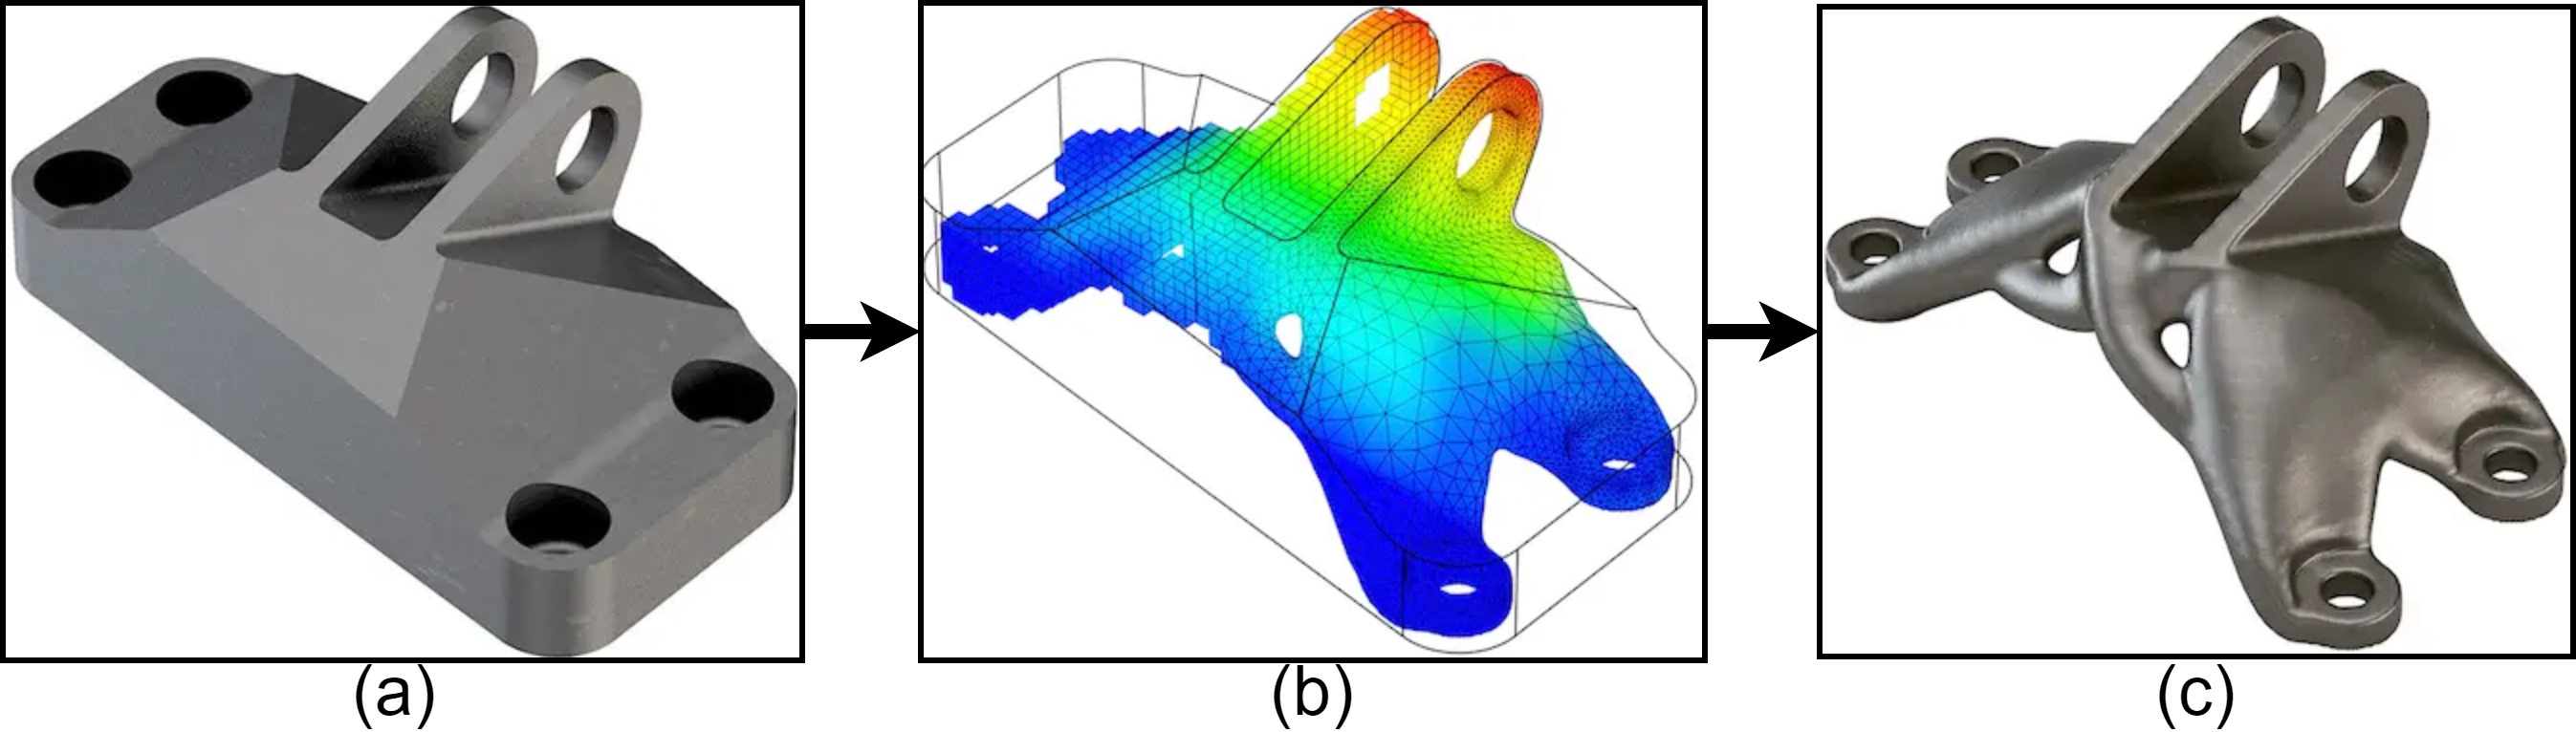
\includegraphics[width=\textwidth]{Figures/Ch_MDP/Fig1_mounted_bracket.png}
    \caption{GE Aircraft mounted bracket challenge \parencite{morgan2014ge} (a) Conventional mounted bracket (b) TO based design analysis (c) Optimized design}
    \label{fig:MDP_Fig1_mounted_bracket}
\end{figure}

In recent years, the significance of TO has increased in the manufacturing industry with the development of Additive Manufacturing (AM) techniques. Many industries are nowadays looking towards advanced design methods like topology optimization and generative design \parencite{atkinson2019manufacturing, Coop2018} for designing future products, including electric machines. Electrical machines are the heart of many appliances, industrial equipment, and systems. They are the foundation of the power industry and the core components of industrial machinery \parencite{lei2017review}. It is estimated that electrical machines use about 43\% - 46\% of total electricity generated globally \parencite{waide2011energy}, resulting in about $6040$ Mega-tonnes of $CO_2$ emission.
This is the largest portion of electricity use among other utilities, as shown in Figure \ref{fig:MDP_Fig2_electrcity_consumption}. Therefore, electric machine energy efficiency is crucial for energy conservation, environment safe-keeping, and global sustainable development. Consequentially, high-efficiency motors will dominate the market development of electrical machines worldwide as discussed in Chapter \ref{chapter:3_RNN}.

\begin{figure}[h!]
    \centering
    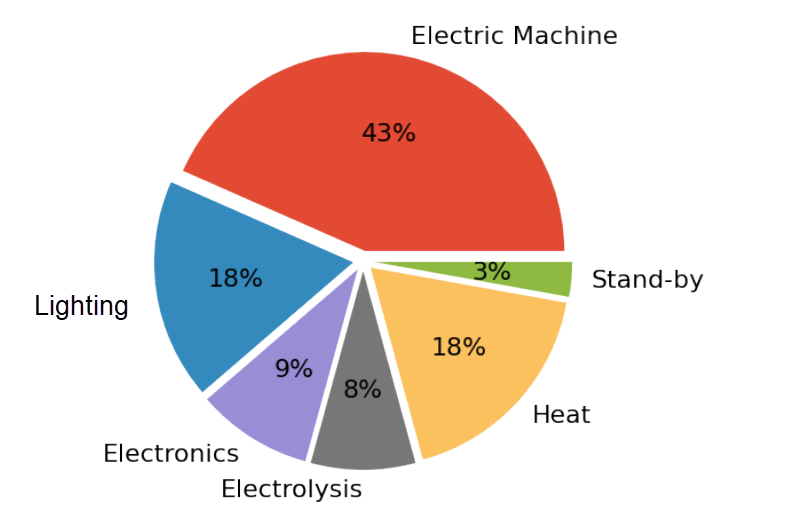
\includegraphics[width=0.85\textwidth]{Figures/Ch_MDP/MDP_Fig2_electrcity_consumption.png}
    \caption{Global Electricity consumption \parencite{lei2017review}.}
    \label{fig:MDP_Fig2_electrcity_consumption}
\end{figure}

In the context of global sustainability, the demand for sustainable alternatives is increasing and electric machines must also fulfill such requirements. As such it is expected that electric machines of the future will be optimized not only physically and technologically but also for their environmental impact. Therefore, their design optimization process becomes more and more complex as more engineering disciplines/domains and constraints are involved, such as electromagnetics, structural, mechanics, and heat transfer \parencite{lei2017review}. This will result in more and more companies in the design and manufacturing industry employing TO in search of environment-friendly designs.

\subsection{Topology Optimization}

The theoretical description  of topology  optimization  originates  from  the mechanical domain,  which  can  be  traced  back  to  Michell’s optimization paper, published in 1904 \parencite{lviiiagm1904limits}. The decade of 1950-60 saw a renewed interest in this sub-field of engineering, with work focused on the optimal layout design of trusses \parencite{cox1958structures, hemp1958theory}.
According to the documented literature, the surge in layout theory research in the 1960s and 1970s led to many significant publications \parencite{cox1958structures, prager1968problems, dobbs1969optimization}. Topology optimization was first applied to electromagnetic (EM) field by \parencite{dyck1996automated},  which  proposed  the Optimized  Material  Distribution method. 

% one or two more sentences on expansion TO in EM

Before discussing TO in-depth, it is essential to understand the motivation behind employing TO over other designing techniques. While designers are known to have excellent imagination, they are prone to biases. The way they have worked in the past influences their future decisions when it comes to modelling. In such cases, the initial geometry can either come from the literature or be based on the designer's knowledge. In either case, the proposed designs tend to be similar to the ones already proved to be efficient. In such cases, even if the design is justified, it might not be the most efficient one. Further, the design requirements may be unique in which case previous knowledge may not exist. In cases, such as these, TO is very useful. TO introduces new shapes and sizes that a designer could not have come up with. These shapes and sizes are generally more efficient at accomplishing the product’s intended task and free from any priors and biases, as decision-making is solely based on input data.

There is no fixed procedure for the design optimization of a device. However, there are some routine steps to be followed. These are briefly described as follows.

\begin{enumerate}
    \item \textbf{Define the domain}: Select a possible design type or topology, which serves as the design domain. Materials and dimensions are set according to the requirements given by the application and users. The main aim of this stage is to find a feasible scheme for a given application that can be explored for an optimal solution.
    
    \item \textbf{Performance and Constraints}: Quantifies the performance/likelihood of the design to be a fit for the requirements.  For example, the performance parameters of an electric device can include efficiency, force, torque, etc., while common design constraints are material and manufacturing costs, volume, etc. The main aim of this step is to obtain several design options that may be suitable for the specific application.

    \item \textbf{Optimization process}: The main target of this stage is to improve the performance of the candidate design proposed in each iteration through some optimization algorithms, to finally converge to an optimal design. This includes implementing multi-physics analysis for each design option generated in the previous step. Due to the multi-physics nature, many engineering disciplines have to be investigated in this step, such as electromagnetics, mechanics, structural, and heat transfer. As an outcome, an optimal design is obtained for a single objective design problem, or some non-dominated designs (also called Pareto optimal solutions) are obtained from a multi-objective design problem.

\end{enumerate}

\subsection{Design Optimization Methodologies}

There are various methodologies designers have employed over the years to find a design which satisfies all the criteria. Some of the techniques popular in literature are:

\begin{enumerate}
    \item \textbf{Sizing (Parametric) Optimization}: Designs are parametrized by a few geometric variables (such as thickness, width, length), as shown in Figure \ref{fig:MDP_size_shape_TO_comparison} (a).
    \item \textbf{Shape (Geometric) Optimization}: Shape Optimization optimizes the boundary and cross-section of the components of a structure. This results in changes of the size and cross-section of the components/members of the structure, as shown in Figure \ref{fig:MDP_size_shape_TO_comparison} (b).
    \item \textbf{Topology Optimization}: Both the shape and the topology of the design can vary without any restriction on the design, as seen in Figure \ref{fig:MDP_size_shape_TO_comparison} (c), where the broken lines show holes in the design.
\end{enumerate}

\begin{figure}[h!]
    \centering
    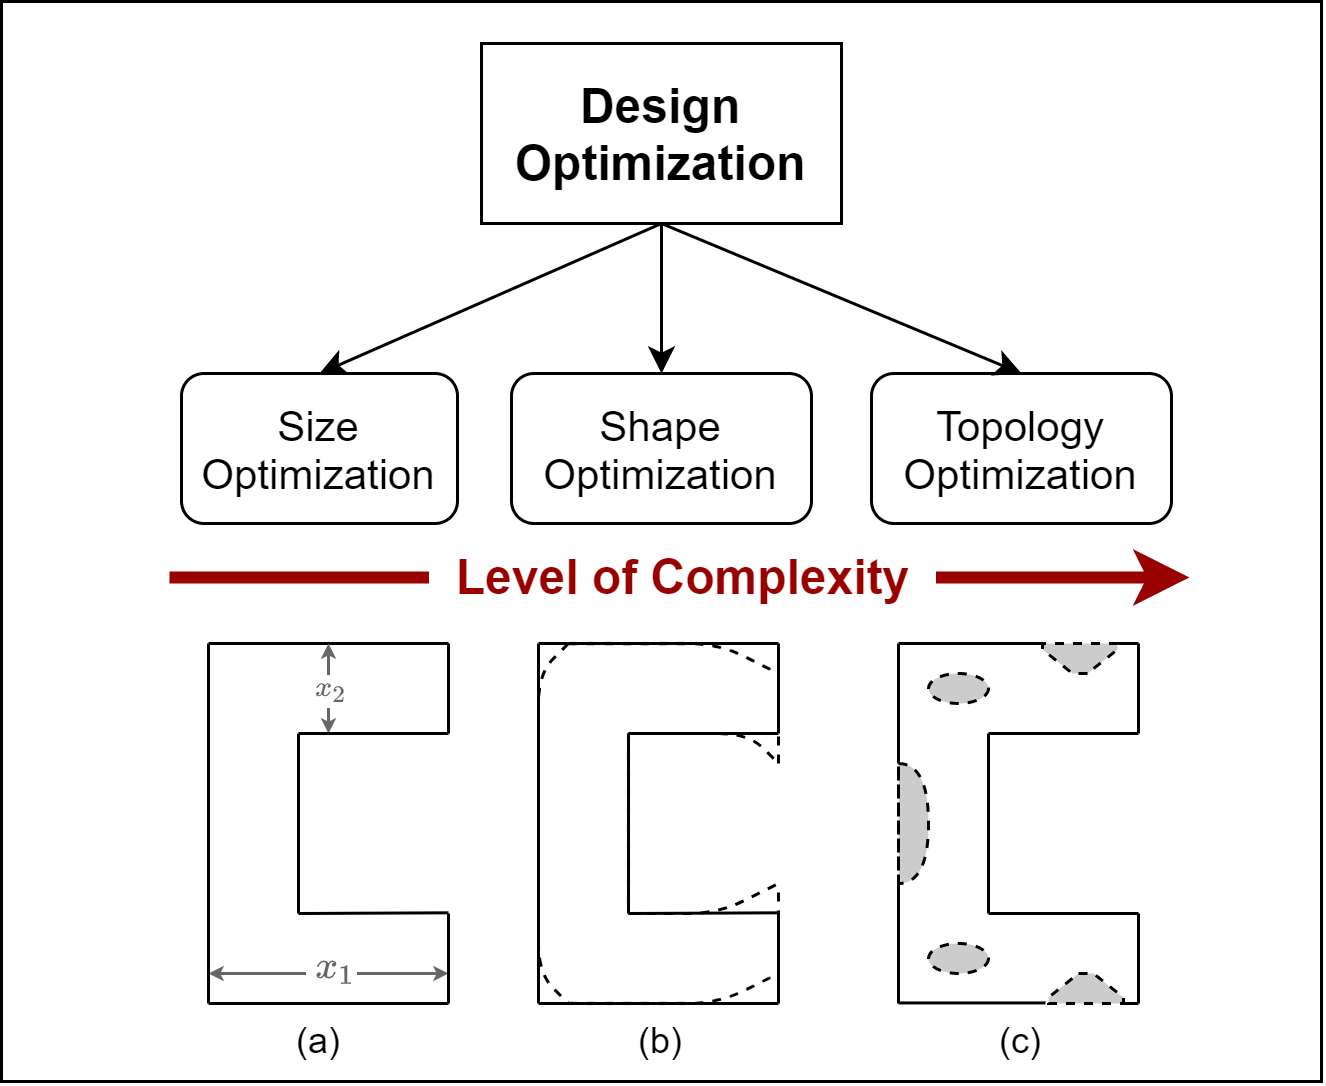
\includegraphics[width=0.75\textwidth]{Figures/Ch_MDP/TO_Parameter_Shape_comparison.png}
    \caption{Different categories of optimal design problems.}
    \label{fig:MDP_size_shape_TO_comparison}
\end{figure}

The design variables associated with sizing optimization are simpler than shape design variables. Sizing will usually increase or decrease the geometrical parameters of a design for example the thickness, which can be very limiting in terms of freedom offered for making changes in the design. Size or Parameter optimization is the most constrained design optimization methodology in terms of the freedom of making change where only pre-defined geometrical parameters are to be changed to find an optimal structure \parencite{haftka1986structural}.
On the other hand, shape optimization offers more freedom than sizing, by modifying the shape of the boundary as shown in Figure \ref{fig:MDP_size_shape_TO_comparison}. However, a major restriction in both types of optimization methodology (shape and size) is that the design topology is fixed and pre-defined \parencite{bremicker1991integrated}.

TO is significantly different from the other two approaches since it necessitates transforming the design optimization problem into a material distribution problem and offers the highest freedom in terms of making changes to the design \parencite{lei2017review}. It is the most flexible of all the categories of optimization methodology and designing with the advantage of free-shape optimization can outperform other optimization routines in terms of the performance if well-tuned \parencite{garibaldi2019free, faria2015design}. Further, TO is used when any prior bias is to be avoided for a design. Due to this capability to generate novel designs TO has become an integral part of modern engineering design and an asset for designers.

\subsection{Optimization Algorithms}
\label{sec:MDP_Optimiaztion_Algorithms}

Unfortunately, transforming the design optimization problem into a material distribution one is also why TO is difficult as the size of search space can be massive. This is related to the number of variables present in the structure to optimize. 

The problem of optimal design is defined based on the following constituents \parencite{allaire2019homogenization}:

\begin{enumerate}
    \item A model, to evaluate (or analyze) the performance of a design.
    \item Objective function: which is to be either minimized or maximized. Also known as a cost function.
    \item Admissible designs/Design domain: defines optimization variables, including constraints.
\end{enumerate}

Before initializing a search for optimal design, it is important to define the design optimization objective, constraints, and parameters. These are usually pre-determined by the user or are derived based on the application requirements and are also dependent on the analysis model used to determine the performance of the designs. As an example, optimization of an electric motor can involve multi-objective requirements to maximize the efficiency based on the constraints of material used and external dimensions.In addition, thermal and structural aspects are also taken into account. In such a case, an electromagnetic analysis based on either FE or MEC has to be performed, along with a thermal network and structural model analysis to calculate winding temperature and resonance frequency. 

Once the objectives and design analysis models are defined, the next task is to choose an appropriate optimization method. Optimization  methods  for  solving  topology  optimization  problems  can  be  roughly divided  into  two  categories:  methods  based  on deterministic  algorithms  and  those  based  on stochastic  algorithms. The deterministic methods use  the  gradient  information  of  the objective  function,  and  have  a  quick  convergence  speed. However, their global search ability is poor, and they are prone to stagnate into optimal local solutions, especially non-convex problems. Moreover,  the performance deteriorates when  dealing  with  multi-objective optimization problems directly \parencite{li2019numerical}. Such methods are also not suitable for topology optimization problems with a large number of design variables.

On the contrary, stochastic  methods  are  optimization  methods  that  use  random search mechanisms. The most popular of such are called Evolutionary Algorithms (EA). They have the following three characteristics:

\begin{enumerate}
    \item \textbf{Population}: EA optimizes the current solutions to generate better solutions. The current set of solutions is called the population.
    \item \textbf{Fitness}: used to quantify which of the solutions is better than others. The fitness value is calculated for each of the solutions using the fitness function.
    \item \textbf{Variation}: Since the next generation of the population is an improvement over the current one, several transformations are performed on the present generation.
\end{enumerate}

Stochastic algorithms are well designed to converge to global solutions of an optimization problem. The injected random variations enable the method to escape from a local optimum; therefore, these methods have a stronger affinity for global optimum than the deterministic algorithms. Further, EA are more suited for mathematical optimization problems with many local extrema. However, the main disadvantage of this kind of method is that the computational cost is high and the convergence speed is slow. This issue becomes overwhelming when a high solution accuracy is desired, resulting in finer meshes. Currently, the global optimization methods commonly applied in the electromagnetic field are genetic  algorithms,  simulated  annealing  algorithms, the tabu  search  algorithm,  particle  swarm optimization  algorithm and quantum  evolution  algorithms.  The  underlying principle  in  these algorithms  is  to  eliminate  the  inferior  solutions and advance the superior  solutions through  the iterative  process of mutation and cross-over,  and  finally  finding  the  optimal  solution  of  the  optimization problem \parencite{li2019numerical}.

\section{Literature Survey}

\subsection{Popular techniques of TO}

Distributing materials in a domain to optimize performance is a significant topic in many fields, such as electromagnetics, solid mechanics, heat transfer, acoustics, fluid mechanics, materials design, and various other multiphysics disciplines, as mentioned earlier. There are several TO methods discussed in the literature, such as density-based methods, homogenization, discrete methods or the ON/OFF approach, and boundary variation methods. These have been applied to the design of Electromagnetic (EM) devices with varying degrees of success and popularity. A brief description of some of the popular TO methods discussed in the literature, such as homogenization methods, density-based methods, boundary-based methods, and discrete methods is included in this section.

\subsection{Homogenization method}

Bendsoe and Kikuchi \parencite{bendsoe1988generating} proposed a method based on the homogenization principle in the late 1980s. The method has received a lot of attention in the field of structural engineering as represented by \cite{bendsoe1993topology} and  \cite{allaire1997homogenization}. This method was first applied in the field of EM in \parencite{yoo2000structural}.

In this methodology, the optimal shape of the structure is transformed into an optimization problem for ideal material distribution. This method uses three design variables (in 2D design space) to describe a microstructure, as shown in Figure \ref{fig:MDP_homo_microStructure}. This results in a large number of variables. 

\begin{figure}[h!]
    \centering
    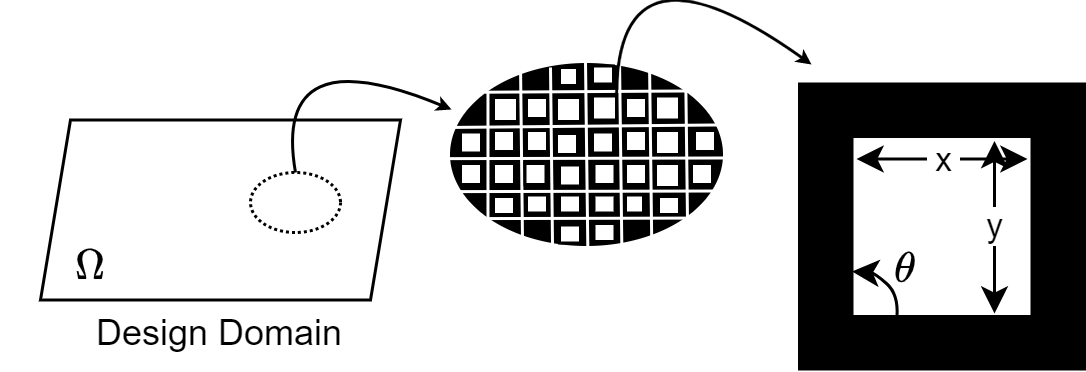
\includegraphics[width=0.95\textwidth]{Figures/Ch_MDP/homo_microStructure.png}
    \caption{Schematic representation of domain discretization used in the homogenization along with a 2-D Unit microstructure with cavity.}
    \label{fig:MDP_homo_microStructure}
\end{figure}

In  homogenization  methods,  the  optimal  shape  of  a  structure  is  transformed  into  the optimal  material  distribution. The homogenization method is based on the concept of relaxation: making ill-posed problems well-posed by enlarging the space of admissible shapes \parencite{allaire2019homogenization}. However, it is not suited for large systems due to a large number of variables and adopts a non-smooth estimate of the topology boundary \parencite{midha_2018}.

In recent times, the homogenization method has received renewed attention, due to progress in the field of additive manufacturing. The ease of manufacturing microstructure materials and homogenization being the ideal technique to deal with microstructure leads to an ideal combination for TO with 3D printing \parencite{guo2013additive}, as shown in Figure \ref{fig:MDP_Crystallon}.

\begin{figure}[h!]
    \centering
    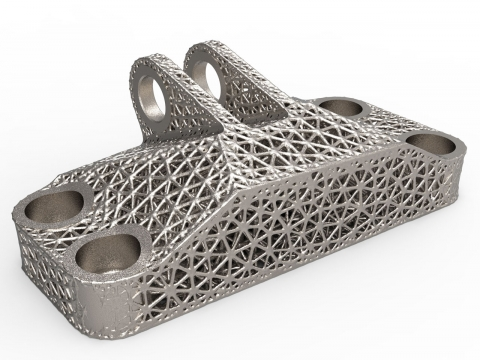
\includegraphics[width=0.45\textwidth]{Figures/Ch_MDP/Crystallon.jpg}
    \caption{Example of a 3D printed lattice structure of a jet engine mounting bracket \parencite{morgan2014ge, allaire2019homogenization}.}
    \label{fig:MDP_Crystallon}
\end{figure}

\subsection{Density method for TO}

Given a fixed domain of finite elements, density based methods optimize the objective  function  by  determining  whether  each  element  should  be either solid  material  or void. Thus it poses an extremely large-scale combination optimization problem. By adopting interpolation  functions  where  the material  properties  are  explicitly  interpreted  as  the continuous design  variables  (usually  the  density  of  materials),  the  discrete  variables  are transferred to continuous variables and an optimizer is used to iteratively steer the solution towards  a  discrete  solid/void  topology.  Usually,  penalty  methods  are  utilized  to  force  the solution  to  a  crisp  “0/1”  or  “solid/void”  topologies.  Further,  regularization  and  filter techniques are adopted to alleviate the checkerboard problem and mesh-dependency issue. The  typical  density  based  methods,  namely  the  Solid Isotropic Microstructure with Penalization (SIMP) method, was proposed  by \parencite{bendsoe1989optimal}. Later \parencite{rozvany1991coc} studied  and  further developed the SIMP method. After it gained popularity in structure optimizations, literature of topology optimization in EM domain based on density-based methods have sprouted in electromagnetics \parencite{yoo2005optimal, byun2002topology, wang2004multi, okamoto20063}.

\begin{figure}[h!]
    \centering
    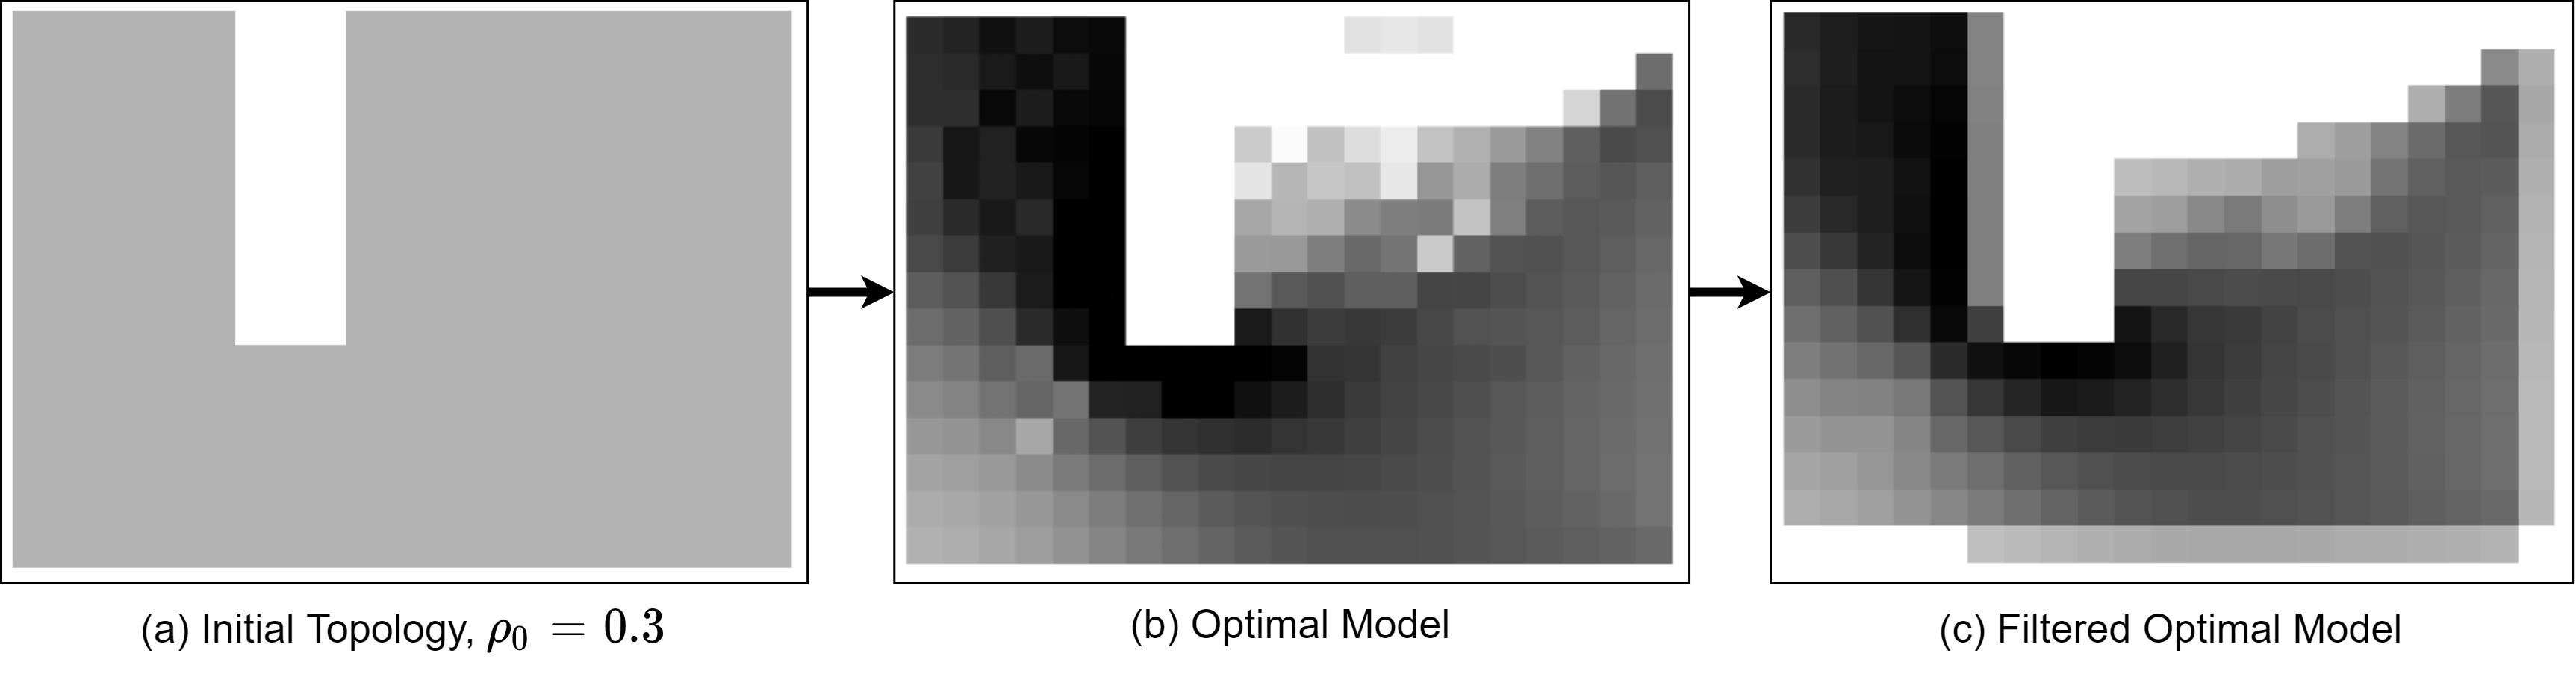
\includegraphics[width=\textwidth]{Figures/Ch_MDP/density_c_core_final.png}
    \caption{(a) Initial Topology, (b) Optimal design from density method, (c) Result with Average filtering \parencite{midha2019selection}.}
    \label{fig:MDP_density_c_core}
\end{figure}

Though  the  density-based  method  takes  the  dominant  position  in  the  topology optimization based on its versatility, effectiveness and ease of implementation (compared to the homogenization approach), it also has a  few  distinct  disadvantages.  In  the  mechanical  domain,  Sigmund  and  Petersson \parencite{Sigmund1998} discussed  the  difficulties  of  the  SIMP  method  such  as  local  optimal,  mesh-dependent structures  and  checkerboard  patterns.  Byun \parencite{byun2004node} and  Okamoto \parencite{okamoto2006investigation} observed  that  the optimized  results  depend  on  the  initial  conditions.  Besides,  one  typical  problem with the density-based method is that of intermediate  density. This is also referred to as grayscales material, regions of intermediate density that are allowed to exist in the optimal configurations. Although  the  penalization (regularization)  scheme and filtering techniques \parencite{midha2019selection} will  eliminate  grayscales  in  a fraction of engineering topology design problems, such filtering schemes crucially depend  on  artificial  parameters  that  lack  rational  guidelines  for  determining appropriate \textit{a priori} parameter values.

\subsection{Boundary based TO}

Apart  from  homogenization and density-based  methods,  boundary  based  methods  are a widely adopted approach to topology optimization, especially in recent decades. The methodology was developed by \cite{osher1988fronts}. The root of  boundary  variation methods  lies  in  shape  optimization  techniques.  Different  from  the density-based  methods  in  which  design  domain  is  parameterized  in  an  explicit  function,  the boundary based methods are based on an implicit function  ($\Phi(x,t) = c$) that defines the structural boundary \parencite{deaton2014survey}. A new dimension is introduced by representing the 2D curve by an intersection between the plane and the surface as shown in Figure \ref{fig:MDP_level_set}. The circular curve ($\Phi(x,t) = 0$) represents the boundary, that is tracked and is specified as the zero level set of the function $\Phi$. The material distribution in the design domain is determined by the values of the level set function ($\Phi$) in the domain, such as 

\begin{align}
    \text{Material}=
    \begin{cases}
      0, & \text{if}\ \Phi < 0 \\
      1, & \text{if}\ \Phi \geq 0
    \end{cases}
\end{align}

\begin{figure}[h!]
    \centering
    \begin{subfigure}[t]{0.4\textwidth}
        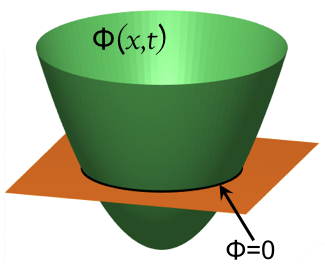
\includegraphics[width=0.75\linewidth]{Figures/Ch_MDP/level1a.png}
        \caption{Intersection of a plane and and a surface}
        \label{fig:MDP_level1a}
    \end{subfigure}
    ~
    \begin{subfigure}[t]{0.4\textwidth}
        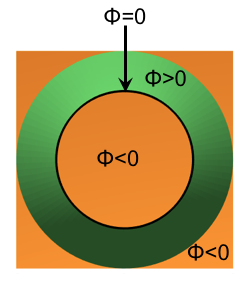
\includegraphics[width=0.75\linewidth]{Figures/Ch_MDP/level1b.png}
        \caption{Top View}
        \label{fig:MDP_level1b}
    \end{subfigure}
    \caption{Represention of a curve by a level set.}
    \label{fig:MDP_level_set}
\end{figure}

Boundary variations methods are mainly employed using level-set and phase-field  methods. In  the  level-set  method,  the  obtained  boundaries  are  still  represented  by  a discretized and unsmooth  mesh  in  the  analysis  domain  unless  alternative techniques are applied. Another  difference  between  density  based  methods  and  boundary  based  methods  lies in  the  product  of  optimization. In  density  based  methods,  the  optimized  topology  usually contain  a lot  of  intermediate  density  elements  where  a post-processing  procedure  for interpreting  topology  is  needed;  however,  the  latter  methods  could  generate  the  optimized topology with crisp and smooth edges. Boundary  based  methods  such as  level-set  method,  also  generates an irregular and toothed  optimized  topology  and  sometimes the  resulting  solutions  are  heavily dependent on the initial state.

\subsection{Discrete Methods}

The ON/OFF or binary discrete methods constitute the discrete approach to TO, where each element in the design space is described using binary digits. In this way, each element can either assume a particular material or remain void (or a background material such as air) \parencite{midha_2018} and thus gray cells/materials are absent in discrete TO methods. In this regard, density-based methods can be seen as translating the discrete problem of material distribution to a continuous form, thus enabling gradient-based optimization algorithms. Although the gradient-based approach is usually faster than stochastic optimization based discrete methods, stochastic methods, such as Evolutionary Algorithms (EA) (used in solving a discrete material distribution problem) offer better optimization capability at finding the global solution, stronger robustness and parallel searching capability, as mentioned in Section \ref{sec:MDP_Optimiaztion_Algorithms}. This is a distinct advantage over gradient-based methods, even though it comes at a cost of high computation demand by frequent objective evaluation calls. A TO design for an electric machine can easily involve more than a 10,000 FE solution in the process of generating the optimal design. The time frame with a 3D FE solver can easily extend to a week. This is a huge computation burden for most designers.

Another drawback of discrete methods is that the optimal solutions contain floating pieces and checkerboard patterns. To overcome this difficulty, either different filtering or smoothing methods are employed \parencite{campelo2008topology} or smoothness of the solution is added as an objective of the optimization process itself \parencite{dupre2014ant}. Various filtering clusters and clan or smoothing techniques are employed to tackle this problem \parencite{campelo2010survey,campelo2008,sato2014}. However, the filtering technique is not reliable and can often lead to an infeasible solution, which can drastically decrease the performance of the optimal design. Further, the filtering technique requires tuning several parameters such as the filter dimensions, thresholds associated with filtering, and the choice of different operating characteristics. Even after tuning, the absence of a single set of parameters of a filtering technique that can give optimal results for all TO problems is missing from the literature.

Even with these shortcomings, the ON/OFF method is popular in the literature due to the convenient implementation of different TO problems, along with easy integration with commercial FEA software. With the help of evolutionary algorithms, it is well designed to exploit global solutions.

\begin{comment}
\subsubsection{3. Why use ON/OFF based TO} 

\begin{itemize}
    \item The  advantage  of  the  ON/OFF  method  is  it's  convenience  to  be  implemented  on different  topology  optimization  problems.  their comparatively separate characteristic of optimization algorithms allows them easy to be implemented accompany with FEA softwares
    \item As  for  heuristic  algorithm  based  methods,  although  they  are  well  designed to exploit  the  global  solutions,  however,  the  computational  cost  is  frequently  high.
\end{itemize}

The disadvantages:
\begin{itemize}
    \item they usually require more computation time to converge, compared to other TO methods discussed in this Chapter. Though with the recent advancements in high power computing it may not be that serious issue.
    For example, consider a PM motor with 10 parameters for optimization by using the GA. Around $40,000$ $(=10 \times 20 \times 200)$ evaluations of the optimization model are required, where 200 is an approximate iteration number for convergence, $10 \times 5$ is a general population size in each iteration(generation) of GA. If each evaluation consists of no-load and load finite element analyses, 40,000 FEM will have to be simulated in the optimization.  For a motor with 3D FEM, it may require half minute or more for one simulation, resulting in at least 40,000 minutes (around 667 hours or 27 days) to obtain an optimal solution. This is a huge computation burden for most designers \parencite{lei2017review}.
    
    \item Another drawback associated with this method is that it results in optimal solutions with floating pieces of material, checker-board or stepping stone patterns. To overcome this difficulty, either different filtering or smoothing methods are employed \parencite{campelo2008topology} or smoothness of the solution is added as an objective of the optimization process itself \parencite{dupre2014ant}. Various filtering cluster and smoothing techniques are employed to tackle this problem \parencite{campelo2010survey,campelo2008,sato2014}. However, the filtering technique is not reliable and can often lead to infeasible solution, which can drastically decrease the performance of the optimal design. Further, the filtering technique requires tuning of several parameters such as the filter dimensions, thresholds associated with filtering and the choice of different operating characteristics. Even after tuning, the absence of a single set of parameters of a filtering technique that can give optimal results for all TO problems is missing from the literature.
    
    \textbf{Different words - same stuff}
    
    good global ability capacitates to  find  the  global  optima  compared  with  deterministic  methods.  However, heuristic  searching  methods  are  far  less  popular  than  density-based  or  boundary-based methods  because  of  their  own  limitations.  One  of  the  most  adverse  factors  is  that  the computational  expense  of  heuristic  methods  is  much  heavier  than  that  of  deterministic methods  (for  example,  gradient  methods). No guarantee for connectivity  of  structure  in  the  stochastic  optimization  process.  Besides,  the  selection  of rational and efficient convergence criterion needs to be paid extra attention.

\end{itemize}

\end{comment}

\subsection{Improvement to ON/OFF TO methodology}

Considering the above-mentioned shortcomings of ON/OFF based TO, several improvements are proposed in this chapter. The first novel contribution of this chapter is a new TO method which ensures that the final optimized solution does not have any checkerboard patterns, perforations or floating pieces of material. Such designs can be difficult to manufacture using conventional subtractive manufacturing methods. Given that AM is quite flexible in terms of what it can manufacture, it is still necessary to check for manufacturability prior to finalizing the design. The proposed TO methodology leverages a sequence-based environment to impose connectivity on cells containing the same material. This new TO method (sequence-based) neither requires any filtering or smoothing technique nor any modification to the optimization objective function for obtaining manufacturable optimal solutions. Furthermore, this method facilitates the application of heuristic tree search-based algorithms such as Reinforcement Learning, which is another novel proposal of this chapter (discussed in Section \ref{subsubsec:MDP_Q_learning}). A few test problems proving the validity of this method are also presented, specifically a C-core actuator in Section \ref{sec:MDP_SynRM_TO_results} \& the rotor of a Synchronous Reluctance Motor in Section \ref{sec:MDP_C_core_Topology_Optimization_Results}. Further, the TO methodology discussed in this chapter will be extended to Chapter \ref{chapter:5_RL} to tackle the issue of generalizing to previously unseen design problems. The ability to generalize will significantly decrease the computation burden associated with an evolutionary algorithm-based discrete TO.

\begin{comment}
\subsection{Problems to study}

We are going to show the working of all the methods for two wide variety of examples.

C-core - Chetan Work

SynRM - Chetan Chapter

Why are these important?
Do mention that Torque ripple is also an issue with SynRM but this work simply focusses on Average Torque.
\end{comment}

\section{Sequence based controller}
\label{section:MDP_Sequence_based_controller}

In this proposed sequence based TO method, a group of cells of the discretized design space serves as a pointer which can move about in the design space (Figure \ref{fig:MDP_controller_movement}), one step at a time and it is referred to as “the controller”. The controller is characterized by its size and the material associated with it. The movement of the controller is decided by choosing from a set of available actions (such as left, right, up or down in the global frame of reference) and the controller leaves behind a trail of material as it moves in the design space. So, the goal is to search for the sequence of actions for the controller such that its movements result in an optimized material distribution in the design space. Figure \ref{fig:MDP_controller_movement} shows the controller moving in a blank grid-based structure. A controller of size 3 fills an area of $3 \times 3 = 9$ cells in the design space. This can be used to modify the problem complexity as a larger size reduces the computation burden of the design optimization problem.

\begin{figure}[h!]
    \centering
    %\includegraphics[width=\textwidth]{Figures/Ch_MDP/controller_movement.png}
    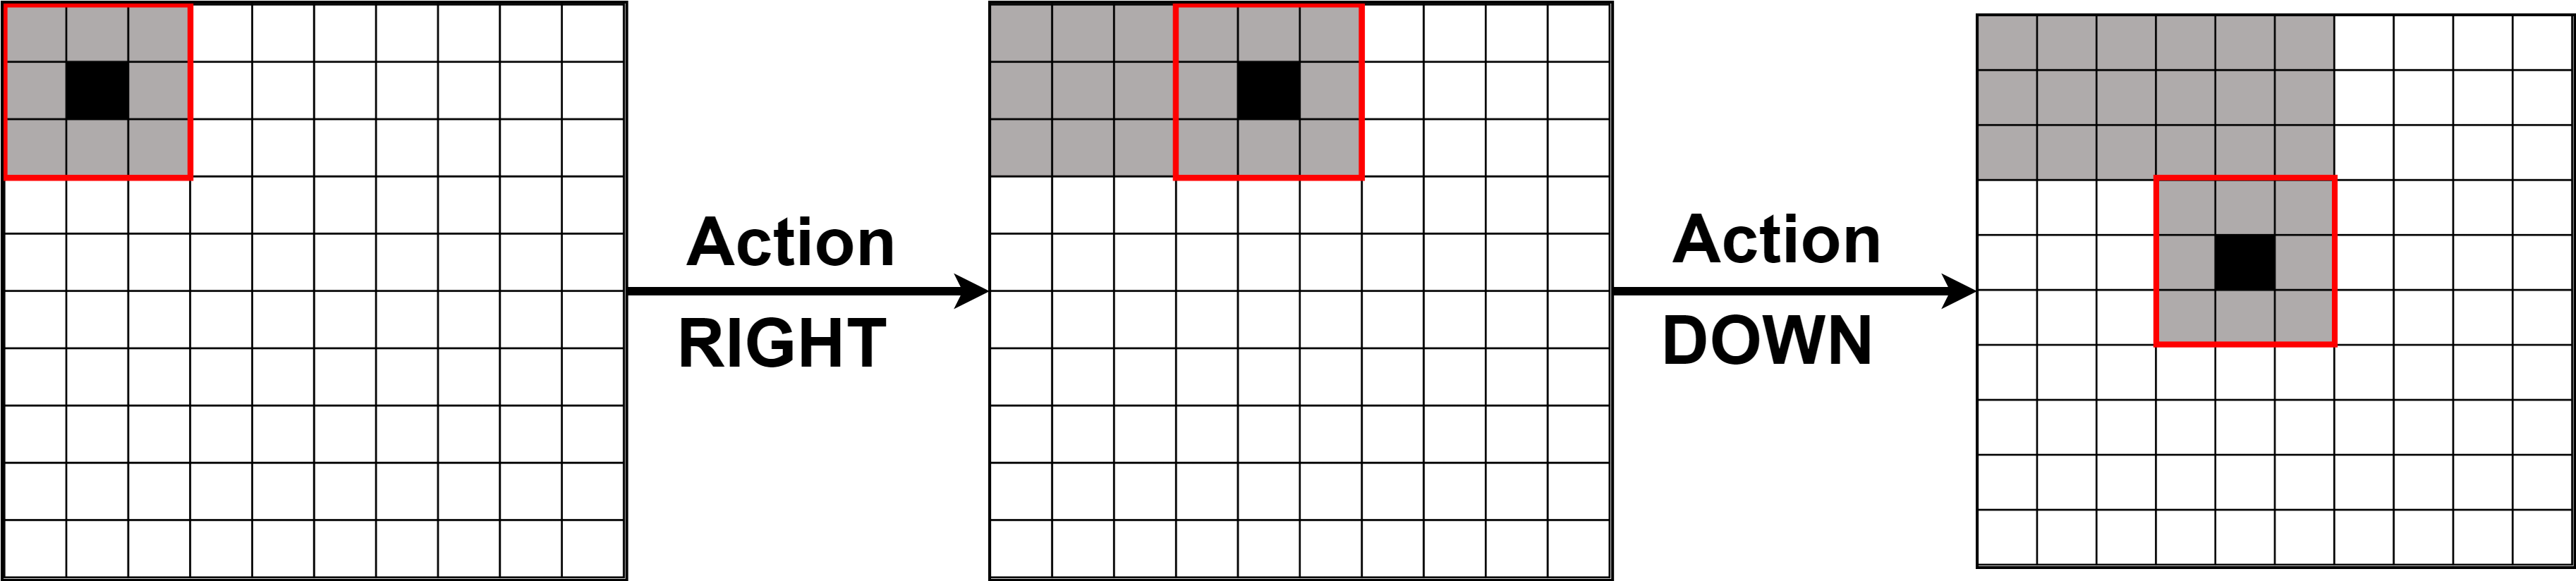
\includegraphics[width=\textwidth]{Figures/Ch_MDP/MDP_movement_final_2.png}
    \caption{The movement of a Controller (size $3 \times 3$) in a design domain.}
    \label{fig:MDP_controller_movement}
\end{figure}

To distinguish the current state representation with any changes made in the future, versioning is maintained such that the current formulation of Sequence based TO methodology is named as SeqTO-\textit{v1}. A future modification named SeqTO-\textit{v2}, will be introduced in Chapter \ref{chapter:5_RL} Section \ref{section:RL_MDP}.

\subsection{The Operation of the Controller}
The controller can move in the design space freely as long as it does not encounter the boundary of the design space. This boundary can be with the excitation source, air or due to symmetry. Further, the controller can be of different size, which will affect the amount of material it can place at a time. The current position of the controller is characterized by a pointer. This is to distinguish the controller from the rest of the material placed in the trail. In the case where the controller is greater than a single element of the grid, the centermost point of the controller is the pointer as shown in Figure \ref{fig:MDP_controller_movement}.

% add a fig to show the pointer
\section{Topology Optimization with SeqTO-\textit{v1}}

\subsection{Genetic Algorithm}
\label{section:results_GA_seqTO}

For the ON/OFF method and SeqTO-\textit{v1}, the design parameters or optimization variables under consideration are discrete, and an optimization technique based on evolutionary algorithms, such as a Genetic Algorithm (GA) works well in such circumstances.

GA is one of the most popular metaheuristic approaches for binary optimization problems, and is inspired by the process of natural selection. In GA, a set of solutions are repeatedly modified using the operations such as `selection', where superior solutions at the current generation are selected for future generations, `crossover', where the selected solutions are combined to evolve into child solutions sharing the characteristics of the parents, and `mutation', where the selected solutions randomly change their values with low probability. The GA algorithm used in this study is based on the work in \cite{midha_2018} and the readers are referred to this material for in-depth explanation. MATLAB’s “Global Optimization” \parencite{matlab, GAtoolbox} is chosen to implement a GA to test the applicability of the proposed environment. 

\begin{comment}

\textit{Genetic algorithm (GA), particle swarm optimization and simulated annealing are some of the popular optimization techniques used with the ON/OFF method. These techniques are also referred to as natural optimization methods, since they attempt to emulate the observable processes in nature that are efficient in optimizing natural phenomena \cite{practGA}. GA belongs to a set of evolutionary computing techniques, which are meta-heuristic or stochastic global optimization methods that either mimic or are inspired by the biological processes of evolution. GA was first proposed by J. Holland \cite{holland}, who provided the theoretical basis for GA through his schema theorem. De Jong showed the use of GA for function optimization and was also first in making a serious attempt to find optimized GA parameters \cite{de1975}. D. Goldberg used GA to solve a difficult optimization problem related to the control of gas-pipeline transmission, thereby proving the method's efficacy and extending its popularity \cite{gold1989, practGA}. Since then GA has been used successfully in numerous applications involving discontinuous, non-linear or non-differentiable optimization objectives, especially involving a large number of optimization variables.
}

\textit{As is evident from its name, GA is based on the principles of genetics and natural selection. It works with a group of potential solutions in the search space, known as a ``population", and tries to evolve this population towards the optimal solution by applying genetic operators in an iterative fashion. A potential solution of the optimization problem is called an individual and it is characterised by a unique chromosome. A chromosome, also known as a genotype, is an encoding of the parameters of an individual and it is often represented as a binary string, although various other data structures are used as well. A chromosome is composed of genes, which in the case of a string representation, are either the individual entries or a group of entries of the string. A fitness value, i.e., the value of the objective function for an individual, is associated with each chromosome that helps in comparing the individuals and selecting the best ones to survive and reproduce, in order to evolve the next generation of the population. }

A GA can start with a random population, and this eliminates dependency on any initial user input. However, to accelerate convergence, sometimes an initial population may be specified if it is known beforehand that the optimal result may lie close to it. This is a choice which is very specific to the expectations and the aim of employing a GA to solve a particular optimization problem.

From a random initial population, the next step is to identify which individuals are best suited to reproduce and evolve the next generation. For this purpose, various genetic operators are applied to the current population. The aim of applying these operators is to efficiently and effectively scout the search space.
The genetic operators commonly used are described as follows:

\begin{itemize}
\item Reproduction
\\The individuals with the highest fitness values in the population are selected to produce offspring and create the next generation. The individuals selected for reproduction are known as parents while the new individuals generated using them are called children. A select few individuals with the best fitness values are retained as they are for the next generation, in addition to acting as parents. This process is known as elite selection.

\item Crossover
\\After reproduction, pairs of parent individuals are randomly selected to mate, and then the genetic information of the pair is swapped at a randomly determined crossover point along the length of each string (chromosome) to create a new child individual, which thus has a combination of genes of both parents \cite{GA2007}.
This process is called crossover and it allows exploitation of the search space to find better solutions.

\item Mutation
\\This involves introducing random changes to one or more genes in the chromosome of a parent individual so as to explore the whole search space and not let the algorithm get trapped in a local minimum. This helps maintain genetic diversity and randomly distribute the genetic information \cite{GA2007}.
\end{itemize}

The genetic operators discussed in the preceding section are applied iteratively, evolving a new generation of individuals every iteration. Theoretically, the GA may be able to find the global optimum value of an objective function only if it is run for a length of time that is long enough to evaluate the fitness of all possible individuals in the design domain. For the size of the optimization problem under consideration ($288$ variables, with each variable allowed to assume a value of either $0$ or $1$, i.e., $2^{288}$ possible individuals in the design domain), it would practically take an infinite length of time. Therefore, it is important to select the conditions that must be satisfied in order to terminate the GA. There are a few criteria which help in deciding when to stop this process. The convergence criteria depend on the optimization problem being solved and a couple of test runs may be required in order to select one.
\begin{itemize}

\item Generation Count
\\The GA is allowed to run for a fixed number of generations and is stopped after this required maximum generation count is achieved.

\item Elapsed time
\\This entails the GA being stopped after a certain period of time has passed, no matter the number of generations reached.

\item Stall Generation limit
\\If there has been no reasonable change or improvement in the fitness value for a fixed number of consecutive generations, the GA is stopped. 

\item Stall Time limit
\\The GA is stopped after a certain time during which there has been no significant change in the fitness value.

\end{itemize}
\end{comment}

\subsubsection{C-core actuator}
\label{section:set_seq_c_core}

% Why C-core important
% useful product
% the flux passing onto armature can be generalized to rotary motion.
% Sources TEAM problem

An electromagnetic actuator is a widely popular device with applications across different industries \parencite{sigmund2001design, choi2009simultaneous, wang2002topology}. A `C’ shaped electromagnet consisting of a coil, a magnetic core, and an armature constitutes a C-core actuator, as can be seen in Figure \ref{fig:MDP_c_core_full} In this structure, the current-carrying coil will produce a magnetic field according to Ampere’s circuit law \parencite{maxwell1861xxv}. The main purpose of the core is to amplify and concentrate the magnetic flux in a well-defined guided path. In this study, a soft magnetic material (M-19) is used as the ferromagnetic material to form the core. The aim is to guide and maximize the magnetic flux flowing through the magnetic core into the armature. The higher the flux connecting the core and armature, the greater will be the pull/force experienced by the armature. The maximization of the flux through the core is a fundamental issue in the design of many electromagnetic devices including actuators, air compressors, electric motors, and generators. As such, the designing of an actuator is a well-studied topic in the field of EM design \parencite{biro2011multi, lim2011topology, lee2012topological, park2012structural, okamoto2015material}. Some of the work focusing on the design of a C-core is used as a benchmark in this study \parencite{park2008magnetic, midha2019selection}.

Applying the Genetic Algorithm (GA) with both ON/OFF and SeqTO-\textit{v1} methodology, to optimize the core of an electromagnetic (EM) actuator so as to maximize the force experienced by the armature. This is done by optimizing the sequence of movements of a controller that consequently results in an optimized material distribution for the core of an EM actuator. The dimensions of the C-core actuator are chosen based on the example considered in \cite{park2009} and \cite{midha2019selection}, as shown in Figure \ref{fig:MDP_c_core_full}. The optimization problem is formulated in Eqn. \ref{eqn:MDP_optimization_problem_formulation} as

\begin{figure}[h!]
    \centering
    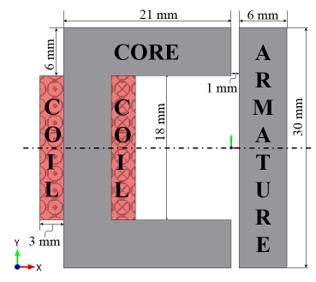
\includegraphics[width=0.35\textwidth]{Figures/Ch_MDP/c_core_full.png}
    \caption{The C - core EM actuator}
    \label{fig:MDP_c_core_full}
\end{figure}

\begin{align}
    \begin{split}
        \underset{\substack{a_i = {0, 1, 2, 3} \\ i = 0, 1, 2, \hdots, m}}{minimize} & \hspace{10pt} f(a) \\
        \text{subject to} \hspace{14pt} K1 \leq & \sum_{j=1}^n (p_j = 1) \leq K2 \label{eqn:MDP_optimization_problem_formulation}
    \end{split}
\end{align}

where, $f(a)$ is the negative magnitude of force experienced by the armature (the negative is imposed to formulate a minimization objective), $a$ is a sequence of actions that governs the controller's movements in the design space. The material distribution in the design space is represented by a vector $p$, which is populated by the action vector $a$. The vector $p$ contains the material property of each cell in the discretized design domain, $m$ is the pre-defined sequence length (length of vector $a$) and is a representative of the freedom given to the controller to explore the environment, $n$ is the length of the material distribution vector $p$, and K1 \& K2 is a limit on the minimum and maximum number of switched ($p_j: 0 \rightarrow 1$) cells permitted in the design space. 

\begin{figure}[h!]
    \centering
    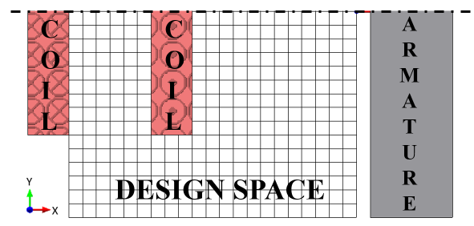
\includegraphics[width=0.60\textwidth]{Figures/Ch_MDP/c_core_half.png}
    \caption{C - core discretized design space}
    \label{fig:MDP_c_core_half}
\end{figure}

\begin{figure}[h!]
    \centering
    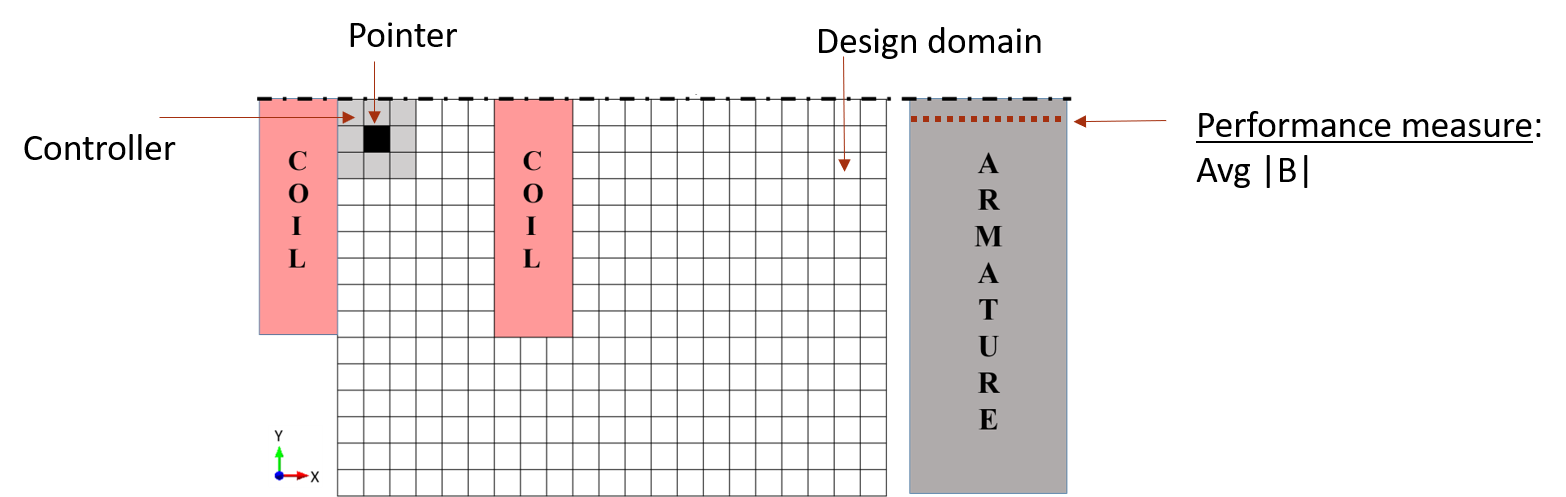
\includegraphics[width=\textwidth]{Figures/Ch_MDP/C_core_controller.png}
    \caption{C-core controller}
    \label{fig:MDP_c_core_controller}
\end{figure}

The depth of both the armature and the core is fixed to 40 mm (the same as that in \parencite{midha2019selection}). The 2-D design space is discretized into 288 square cells of size 1 mm and symmetry about the x-axis is utilized to reduce the size of the design space as shown in Figure \ref{fig:MDP_c_core_half}. The material in these cells is permitted to switch between air ($p_i=0$) and electrical steel ($p_i=1$), depending on the movements of the controller.

A conventional half-symmetric C-core shape consists of 180 electrical steel cells in the discretized design domain. $K2$ is set to 180 and serves to enforce the volume constraint on the electrical steel. $K1$ is set to 80 to ensure that the controller explores the design space. The value of $m$ (length of $a$) is an important hyperparameter which must be decided beforehand and it also depends on the selected controller size. It is equal to the maximum number of steps (actions) that the controller is allowed to take when it moves in the design space. This value should be such that the controller is able to take enough steps to fill in at least the allowed number ($K2$) of cells with material. Usually, $m$ is chosen such that the controller is able to fill a little more than $K2$ number of cells in the design space. This is done to account for the steps taken by the controller which do not result in any additional material in the design space. Initially, air ($p_i=0$) is assigned to all the cells in the design space. A starting location for the controller is specified beforehand and it remains constant throughout the optimization process. This method also allows for the selection of different starting positions of the controller in the design space.

Some of the GA’s parameters are directly dependent on the TO controller configuration. The number of design variables for GA is set equal to $m$. The population size is selected to be a multiple of the number of design variables.

\subsection{Tree Search Algorithms}
\label{section:MDP_TD_learning}

Apart from the advantage of generated designs which are free from checkerboard patterns and ensuring connectivity of material in the design domain, sequence-based TO also provides the capability to use algorithms which make decisions as a series of sequences such as tree search algorithms like Temporal difference (TD) learning, Monte Carlo (MC) algorithms and others that are related to Dynamic Programming (DP) \parencite{sutton1988learning}. 

The main advantage of exploring these algorithms is the stark difference they pose in relation to evolutionary algorithms. Table \ref{tab:MDP_comp_GA_v_RL} lists a comparison of Evolutionary Algorithms and sequence based decision making such as TD-learning. It should be noted that these sequence-based decision making algorithms come under the wide topic of Reinforcement Learning (RL). Reinforcement learning is characterized by the fact that the learning system’s actions (movement of the controller) influence its later inputs (states). The learning system does not have direct instructions on the optimal actions to take, and no knowledge of the consequences of actions, including reward signals, and how they play out over extended period of time \parencite{sutton2018reinforcement}. Since this work only deploys a TD-learning based algorithm, the general algorithms in RL will not be discussed here.

% Please add the following required packages to your document preamble:
% \usepackage{graphicx}
\begin{table}[h!]
\centering
%\resizebox{\textwidth}{!}{%
\begin{tabular}{|c|c|}
\hline
\textbf{Reinforcement Learning}                                                                                                                                                & \textbf{Evolutionary Algorithms}                                                                                                                    \\ \hline \hline
\begin{tabular}[c]{@{}c@{}}One agent trying to learn from \\ both positive and negative actions\end{tabular}                                                                   & \begin{tabular}[c]{@{}c@{}}Starts with many agents, \\ but only strong ones survive\end{tabular}                                                    \\ \hline
\begin{tabular}[c]{@{}c@{}}Learns from both positive and\\  negative rewarding actions\end{tabular}                                                                            & \begin{tabular}[c]{@{}c@{}}Only learns the optimal solutions. \\ Negative or sub-optimal solution \\ information is discarded and lost\end{tabular} \\ \hline
\begin{tabular}[c]{@{}c@{}}Good for problems that can be \\ represented as a Markov \\ Decision Process (MDP) \\ (Section \ref{section:MDP_MDP})\end{tabular} & \begin{tabular}[c]{@{}c@{}}Good for problems where \\ loss function is non-differentiable.\end{tabular}                                             \\ \hline
%Local convergence                                                                                                                                                              & Global convergence                                                                                                                                  \\ \hline
\end{tabular}%
%}
\caption{Comparison between Evolutionary Algorithms \& Reinforcement Learning}
\label{tab:MDP_comp_GA_v_RL}
\end{table}

\section{TD Learning}
\subsection{Markov Decision Process}\label{section:MDP_MDP}

A Markov Decision Process (MDP) is a discrete-time process that converts a given `task' to a sequential problem. The key entities of an MDP are the environment, state, action, and reward. The controller interacts with the environment in discrete steps. At each step (denoted by `$t$' in subscript) the controller receives a `state' from the environment. The `state' contains sufficient information regarding the current material distribution in the design domain for the controller to interpret and make a rational decision (action). Based on the action that the agent took in a state ($s_t$), the environment provides a feedback in the form of a reward ($r_t$). Contrary to the word `reward', the agent can also be penalized for an illegal or a bad move with a penalty (through a negative reward). The environment also provides the next transition state ($s_{t+1}$). Actions influence the reward as well as the future states and through that future rewards. The algorithm revolves around exploring the environment to learn the transition from one state ($s_t$) to another ($s_t'$), based on an action ($a$),($s\rightarrow s'$). This transition will result in a reward signal ($r_t$). This reward at each step is a scalar quantity $r_t \in \mathds{R}$.

In an MDP, state transition and reward function are solely dependent on the current state and the chosen action and is independent of the previous states and actions. Some states are set as terminal states, and tasks reaching them are terminated.

\begin{figure}[h!]
    \centering
    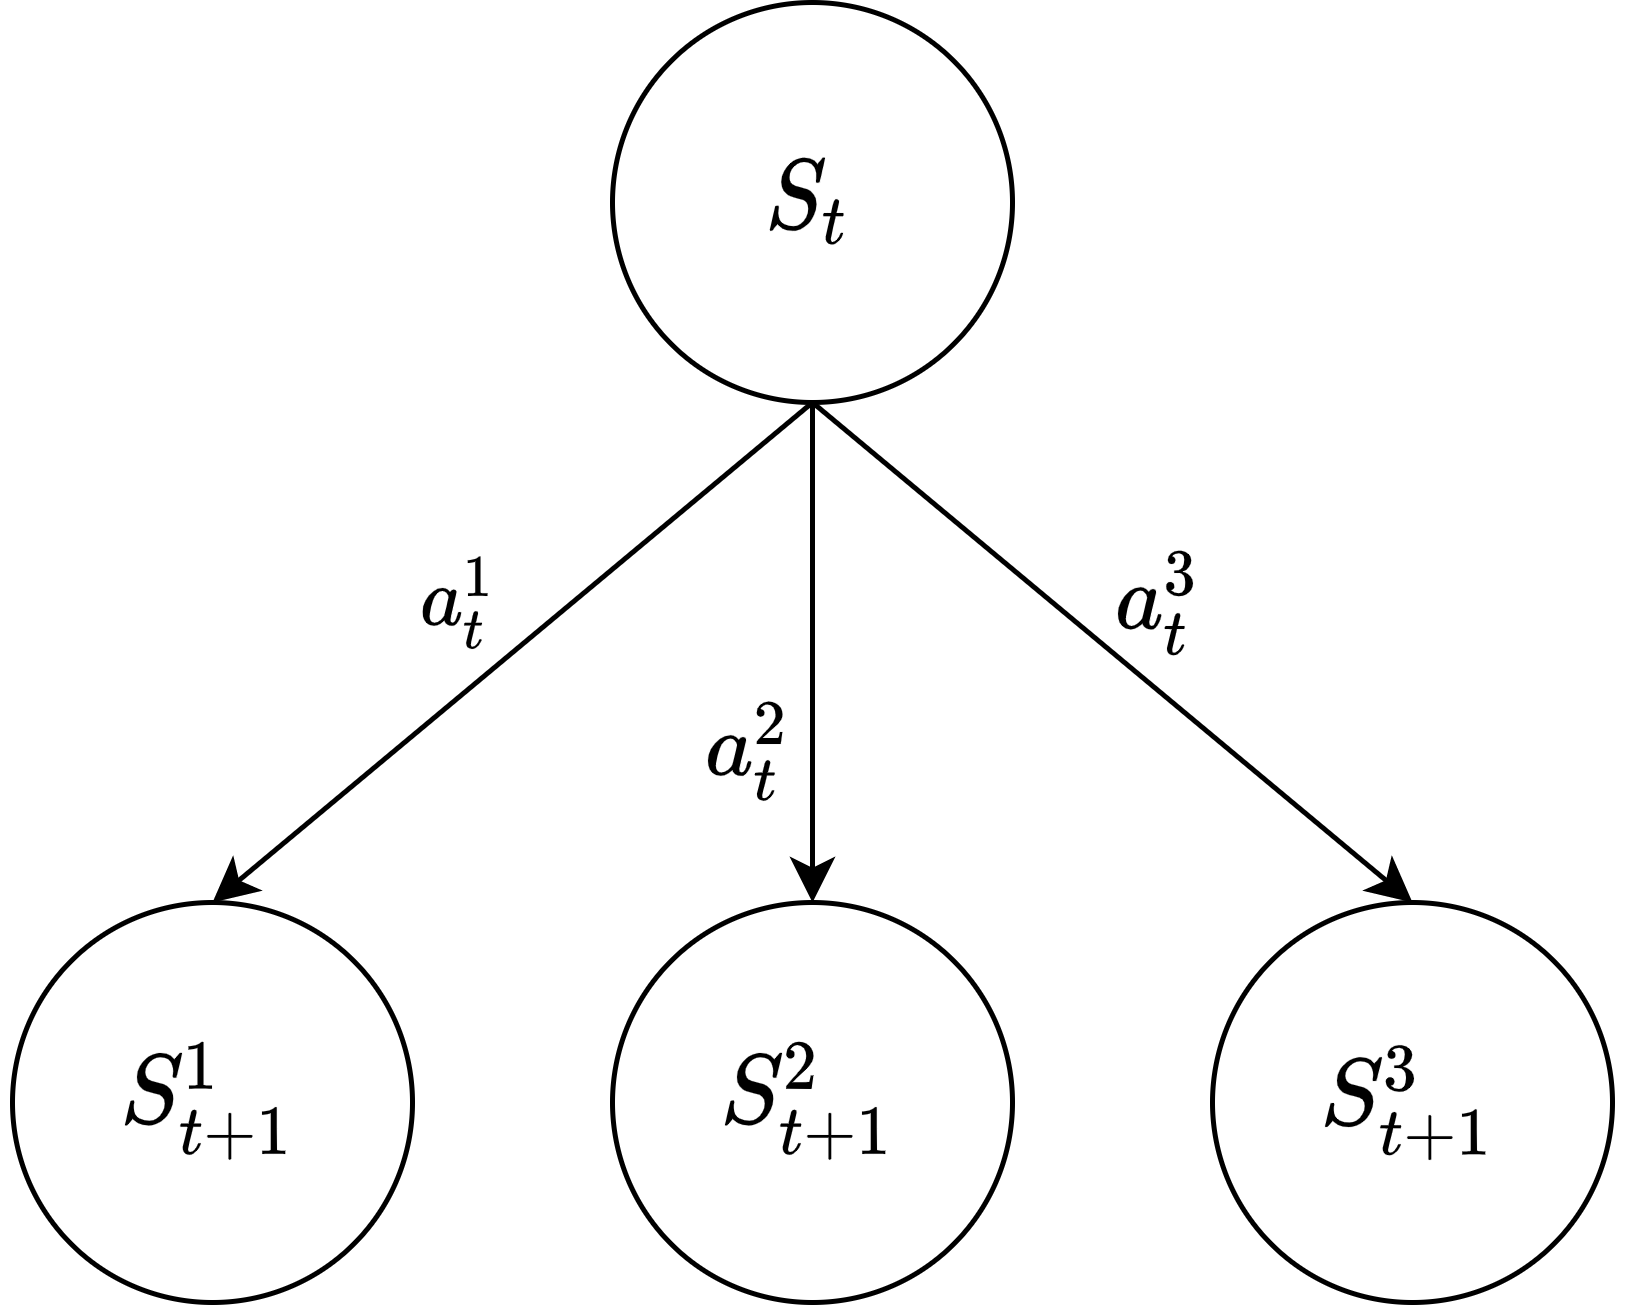
\includegraphics[width=0.35\textwidth]{Figures/Ch_MDP/MDP_state_transition.png}
    \caption{State Transition ($s_t, a_t, s_{t+1}$)}
    \label{fig:MDP_state_transition}
\end{figure}

\subsubsection{Policy}
The choice of action has an impact on both the immediate reward and the next state. Policies determine how an agent selects these actions. A `policy' is a distribution over actions for all possible states. A deterministic policy maps each state to a single action from the action set, thus:
\begin{align*}
    \pi(s) = a
\end{align*}
where $\pi$ is a deterministic policy and $\pi(s)$ represents the action selected in the state ($s$) by the policy ($\pi$). A deterministic policy here can be represented in a tabular format. The same action can be selected in multiple states, however, some actions may not be favorable and are not selected at all. The distribution of actions is independent of each other, for all possible states. On the other hand, a stochastic policy is one where multiple actions can be selected with a non-zero probability. The set of available actions in each state is the same but the probability distribution varies. In an ideal MDP, a state has all the information for decision making. This chapter deals with deterministic policies and stochastic policies will be discussed in Chapter \ref{chapter:5_RL}.

\subsubsection{Episodic Task}
Another important criterion is to determine if the task is episodic or continuous. Since the controller has a limited amount of material (volume constraint) and we want the controller to limit the number of function (FE in this case) calls, the design optimization setup limits the length of an episode to be sufficient to move around and place the given volume of material. It should be checked that the agent has enough leeway in the number of steps in an episode, to be able to explore the vast design space. A guideline, in this case, would be to identify the number of steps needed to come up with the conventional geometry using the MDP formulation and allow the controller to spend double the number of steps in the design domain for each episode. This will give the agent a sufficient amount of steps to explore the design space.  

\subsubsection{Reward Formulation}
The dynamics of the MDP have to be such that they result in the successful creation of an optimal geometry subject to a material (volume) constraint. The goal should be to translate an agent's behavior to maximize the reward. This means maximizing the immediate reward and the cumulative reward in the long run (such as an episode). The agent's learning has to balance the short term and long term goals. The reward function should be seen as a way to communicate with the agent as to what to achieve. 
In such a case, the obvious reward function will be the performance (objective) criteria that is being maximized/minimized. For a C-core, it will be the force experienced by the armature at any given step of the MDP. 
However, it was observed that sometimes the force experienced can be noisy and not accurate. This was attributed to circumstances when the design domain contains very little material (usually at the start of an episode), the force value will be small and it will become difficult to distinguish two sparsely populated (with material) design domains. Thus, it was decided that the magnetic field distribution values in the C-core armature (Figure \ref{fig:MDP_c_core_controller2}) is a far more robust indicator of performance. Further, this can work as a substitute for force value as it is directly proportional to the magnetic field lines passing through the armature. 

\begin{figure}[h!]
    \centering
    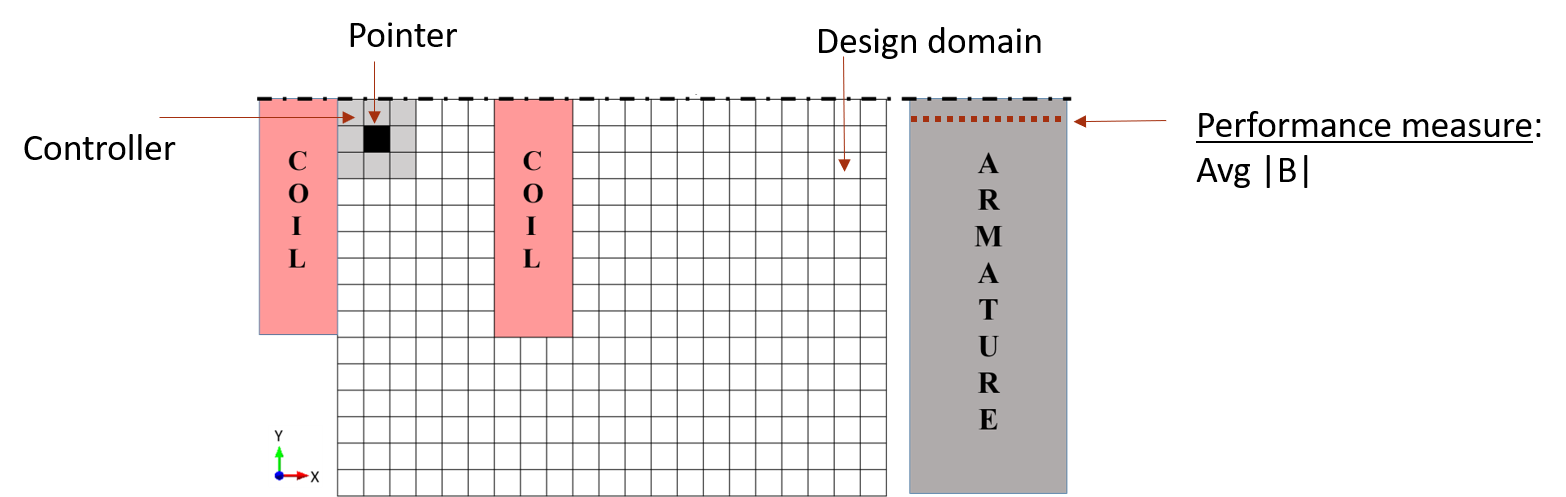
\includegraphics[width=\textwidth]{Figures/Ch_MDP/C_core_controller.png}
    \caption{C-core controller}
    \label{fig:MDP_c_core_controller2}
\end{figure}
Maximizing the total return at time `$t$', is simply the sum of rewards the agent will receive after time `$t$'.
\begin{align*}
    G_t \doteq R_{t+1} + R_{t+2} + \hdots + R_{N}
\end{align*}
where $G_t$ is called the return.

\subsubsection{MDP Dynamics}
An important property to remember is that the future states and reward only depend on the current state and the action. This is a Markov property that needs to be satisfied for a proper MDP. For enabling actions that depend on the agent's behavior (action taken) in the previous step, it is important to include this information in the state representation without violating the Markov property. This is achieved through keeping a trace of past distribution of the design domain and material distribution in the state representation. The Markov property means that the present state is sufficient and remembering earlier states would not improve predictions about the future. This is an important property as there can be multiple ways of representing the state for a discrete design domain for TO, as shown in Figure \ref{fig:MDP_state_repr_original}, \ref{fig:MDP_state_repr_2} \&  \ref{fig:MDP_state_repr_3_Bfield}. In this chapter only the state representation shown in Figure \ref{fig:MDP_state_repr_original} will be used with the RL and GA algorithms. The other state spaces (Figure \ref{fig:MDP_state_repr_2} \&  \ref{fig:MDP_state_repr_3_Bfield}) will be used in Chapter \ref{chapter:5_RL} with advanced algorithms in RL.

\begin{figure}[h!]
\centering
\begin{minipage}{.45\textwidth}
  \centering
  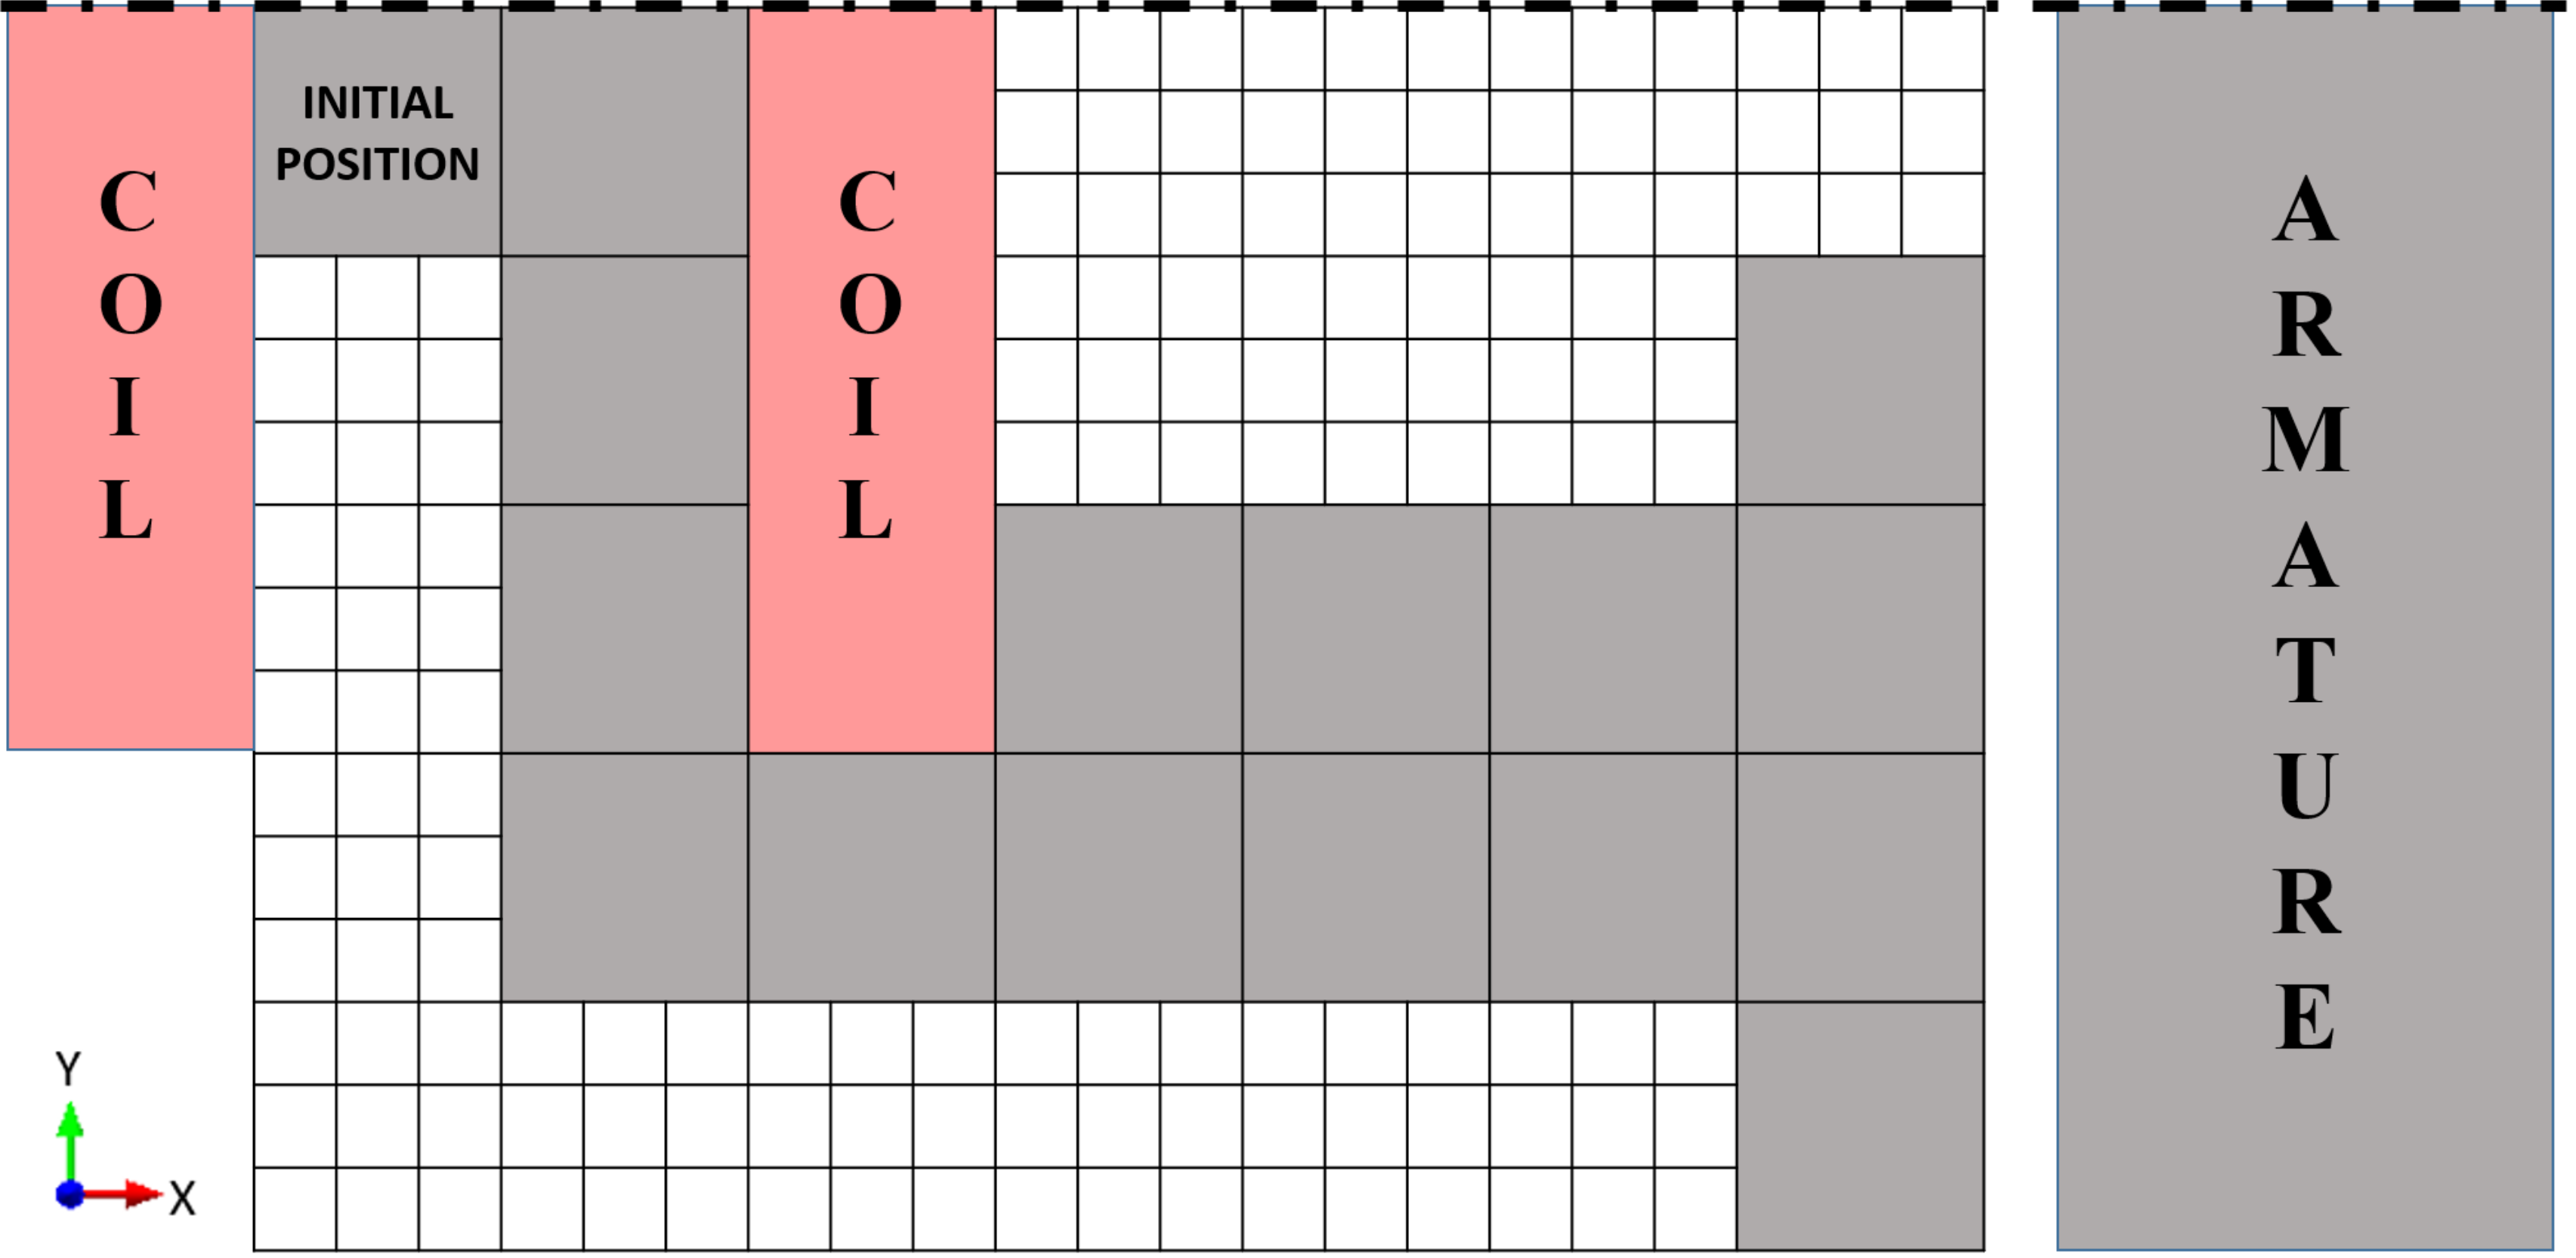
\includegraphics[width=0.8\linewidth]{Figures/Ch_MDP/state_repr_1.png}
  \captionof{figure}{Discrete design domain as the state space}
  \label{fig:MDP_state_repr_original}
\end{minipage}%
\begin{minipage}{.45\textwidth}
  \centering
  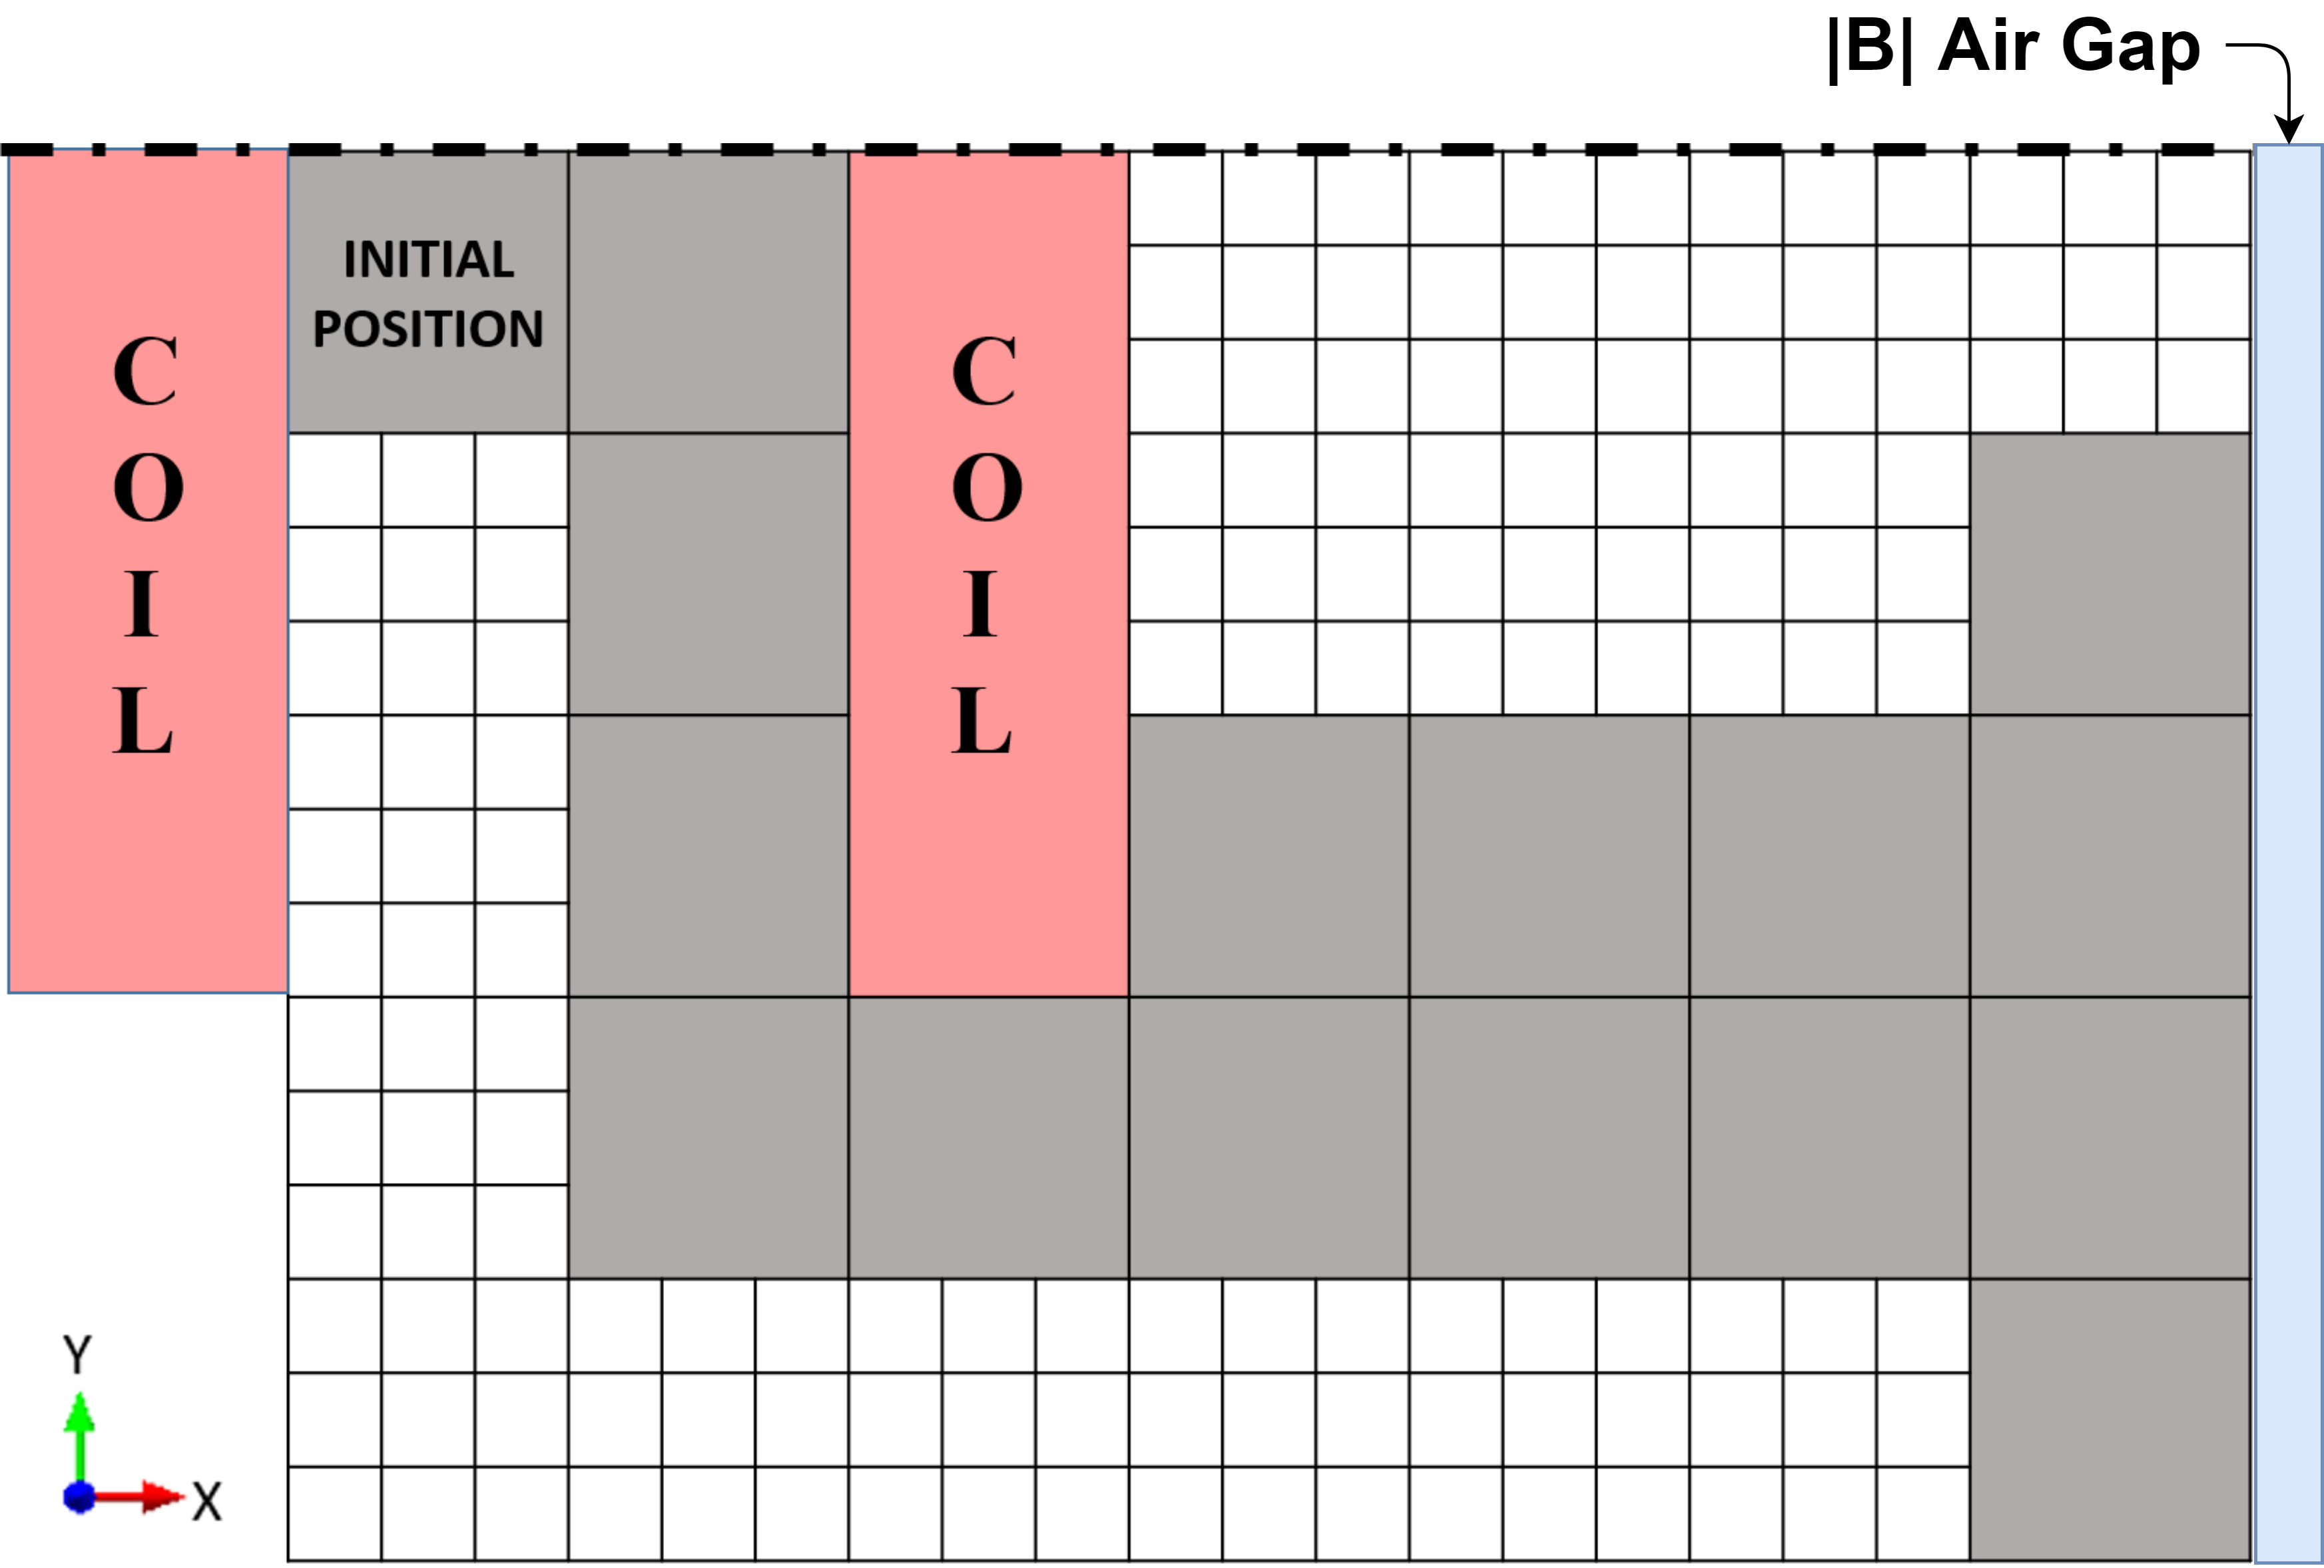
\includegraphics[width=0.8\linewidth]{Figures/Ch_MDP/state_repr_2.png}
  \captionof{figure}{Discrete design domain with the $|B|_{airgap}$ as the state space}
  \label{fig:MDP_state_repr_2}
\end{minipage}
\end{figure}

\begin{figure}[h!]
    \centering
    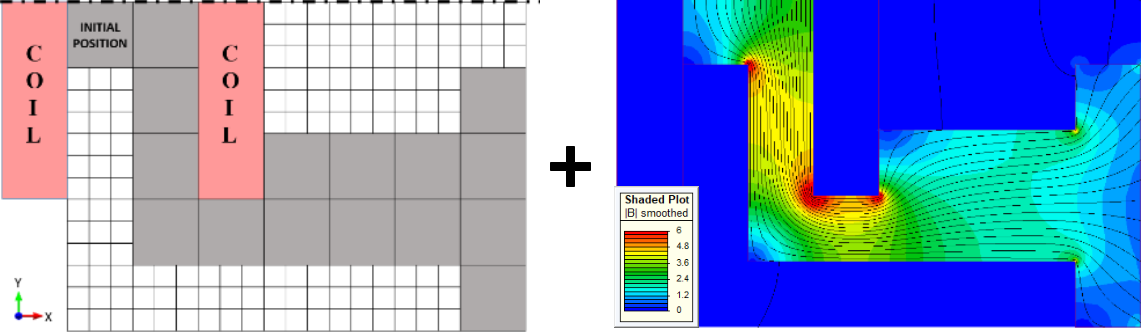
\includegraphics[width=0.95\textwidth]{Figures/Ch_MDP/state_repr_3_mdp.png}
    \caption{Discrete design domain  along with the $|B|$ in the design space as the state space}
    \label{fig:MDP_state_repr_3_Bfield}
\end{figure}

It should be noted that the MDP formulation can be designed in many different ways. It is very abstract and flexible. Formulating an MDP for any task requires knowledge of system dynamics of the electromagnetic problem, agent training, and the reward formulation. Necessary changes have to be made for adapting this work to other tasks. A number of modifications in the current formulation of SeqTO-\textit{v1} will be discussed in Section \ref{section:RL_MDP}. Further, we have not delved into the process of accounting for the complexity of the problem. The set of states and actions are countable, the value will be very high and is $\infty$ for the reward set. 

\begin{figure}[h!]
    \centering
    
\includegraphics[width=\textwidth]{Figures/Ch_RL/c_core_negative_error.png}
    \caption{Scenario for a negative Reward ($R_t$)}
    \label{fig:RL_neg_reward}
\end{figure}

\begin{figure}[h!]
    \centering
    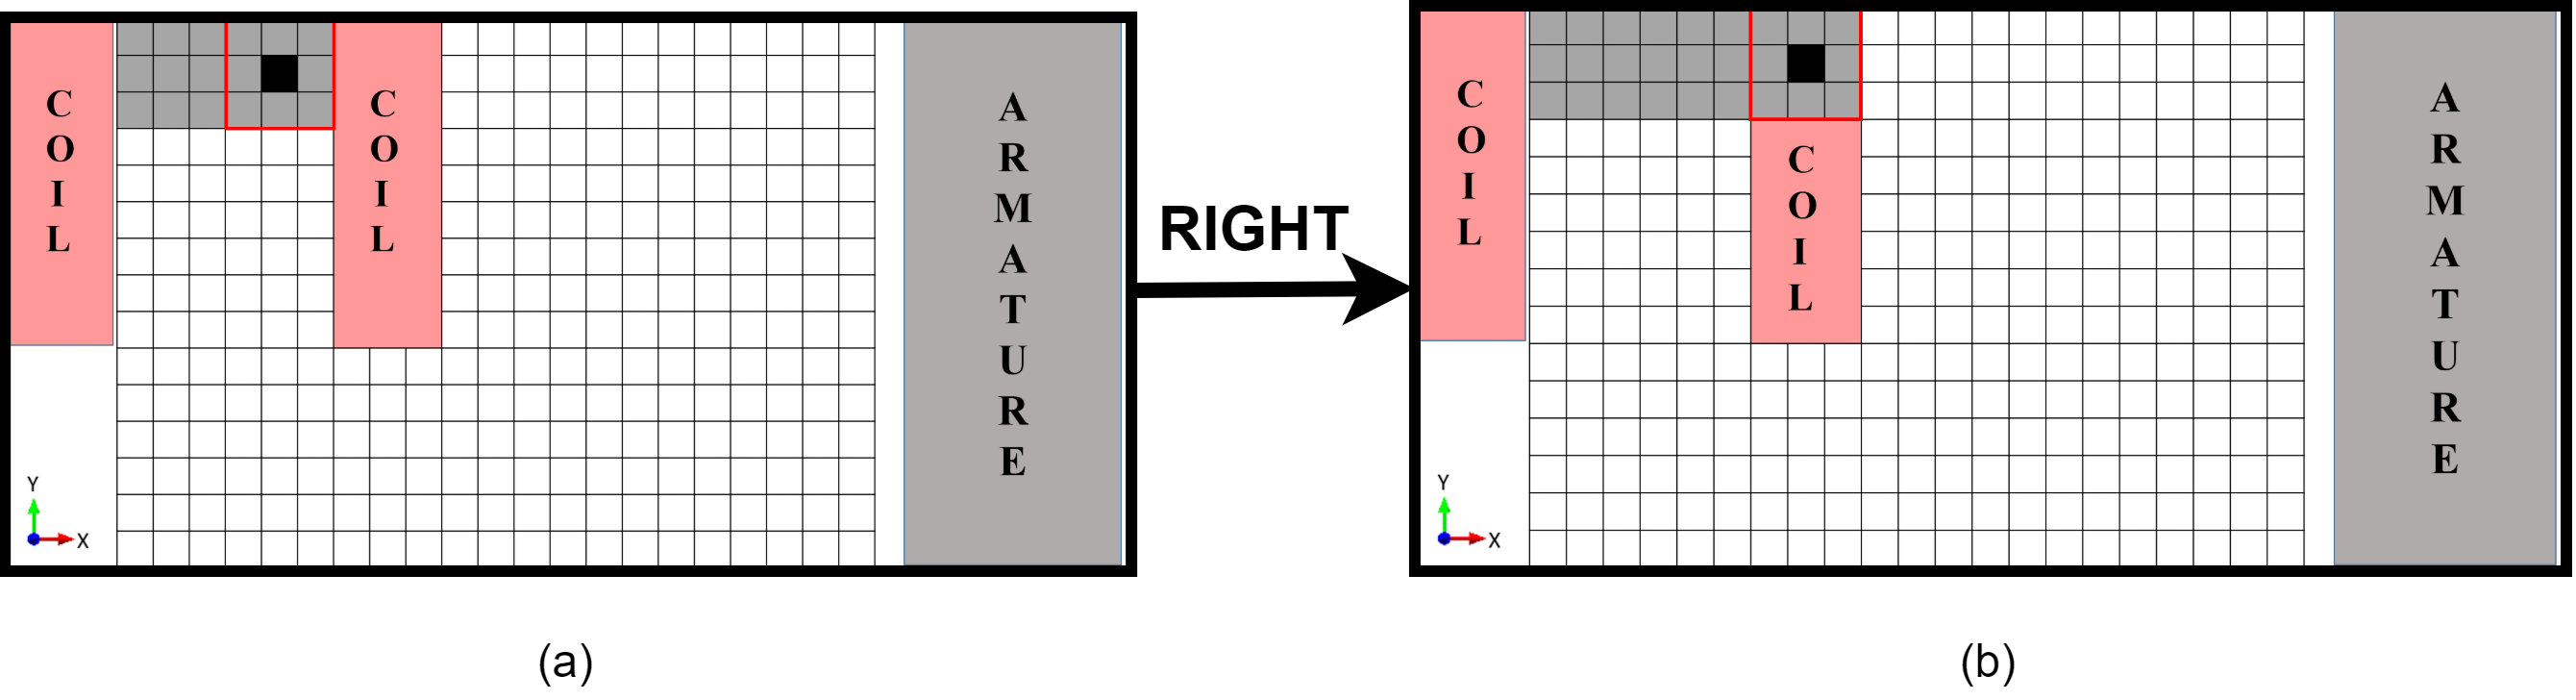
\includegraphics[width=\textwidth]{Figures/Ch_RL/Coil_error.png}
    \caption{Possibility of a design error due to the controller moving out of the designated design space.}
    \label{fig:RL_coil_error}
\end{figure}

\subsection{Value functions}
\label{section:MDP_QL-Value_Function}

The reward function captures the notion of short term gain. However, the agent should achieve the most reward in all the subsequent state trajectories, i.e, in the long term. The Value function, either $Q(s,a)$ or $V(s)$, formalizes this. The value function can be represented in two forms:

\begin{itemize}
    \item \textbf{Action value function }$Q(s, a)$: A Q-Value ($Q(s, a)$) is a measure of all the rewards the agent shall receive till the end of the episode, starting from the state ($s$) and after performing an action ($a$). This cumulative reward function can be discounted based on the temporal position of the reward from the current step ($t$).
    \item \textbf{State value function} $V(s)$: On the other hand, the State value function ($V(s)$) is the expected value of all possible future rewards, on all possible actions.
\end{itemize}

It is preferable to use the Action value function ($Q(s, a)$) for this work. This preference is based on the knowledge that a transition from one state to another can be performed in more than one way. Further $Q(s, a)$ is more useful for comparing the different actions available in a state. 
The agent-environment interaction generates a trajectory of experience consisting of states, action, and rewards. 
TD-learning uses the value associated with each state-action pair to utilize all the experience ($s, a, s', r$) generated by the agent.
The value of the state-action pair is the expected return ($G_t$) when that action is taken

\begin{align}
    Q(s, a) \doteq \mathds{E}_{\pi} [G_t|s_t = s, a_t=a] \label{eqn:MDP_Q_function_intro}
\end{align}

For an episodic task, the learning algorithm needs to wait until the end of the episode to work with the absolute/true value of the `return' for every step in the corresponding episode, since the `return' ($G_t$) depends on all the reward obtained from $t$ - step onwards.

\begin{align}
    G_t \doteq R_{t+1} + R_{t+2} \hdots R_n
\end{align}

This approach is the key to Monte Carlo (MC) based methods. 
In MC, there is no guarantee that the agent will visit all the possible states, along with the other issue of waiting for the end of an episode to update the value function ($Q(s,a)$) \parencite{singh1996reinforcement}. 
However, there is another approach that uses bootstrapping, which is based on recursive use:
\begin{align}
    G_t \doteq R_{t+1} + G_{t+1} \label{eqn:MDP_recursive_return}
\end{align}

In a similar fashion as Eqn. \ref{eqn:MDP_recursive_return}, the value function (Eqn. \ref{eqn:MDP_Q_function_intro}) can also be updated as:
\begin{flalign}
    \begin{split}
    Q(s_t, a_t) & \doteq \mathds{E}_{\pi} [R_{t+1} + G_{t+1}|s_t = s, a_t=a]\\
    Q_{\pi} (s) & = R_{t+1} + Q_{\pi} (s_{t+1}, a_{t+1}) \label{eqn:MDP_Qpi_46}
    \end{split}
\end{flalign}

Compared to MC-based methods that wait until the end of the episode to update all the corresponding value functions, bootstrapping-based methods (such as TD-learning) learn incrementally and throughout the episode.
However, the disadvantage of the TD-learning approach is that the incremental updates can have higher variance compared to the true return based approach of MC methods. It has been shown practically that bootstrapping based methods converge faster but may be off the target, or not properly learn the true return values \parencite{sutton2018reinforcement}. For faster learning, we want to update towards the return but not wait for the episode to complete, so the empirical (true) value of the return at a time `$t$' is replaced with the reward and the estimate of the return from the next state. This way the updates to the value function ($Q(s_t, a_t)$, performed by the learning algorithms are faster.

\begin{align}
    Q_{\pi}(s_t, a_t) & \leftarrow Q_{\pi}(s_t, a_t) + \Big[G_t - Q_{\pi}(s_t, a_t) \Big]\\
    Q_{\pi}(s_t, a_t) & \leftarrow Q_{\pi}(s_t, a_t) + \Big[R_{t+1} + \max_{a'} Q_{\pi}(s_{t+1}, a') - Q_{\pi}(s_t, a_t) \Big]
\end{align}

TD updates the value of one state ($Q(s_t, a_t)$) towards it's own estimate of the value in the next state ($Q(s_{t+1}, a_{t+1})$).  As the estimated value of the next state improves, so does the target.

To overcome the disadvantage of higher variance in the return due to incremental updates in TD learning, the rewards are adjusted by weighing the rewards based on their importance over time. The farther in future a reward is received, the lesser is it's importance while calculating the return at time `t' ($G_t$). This is controlled using discount factor ($\gamma$). 
The discount factor helps reduce the degree to which future rewards affect the current value function estimates; thus stabilizing the learning.
The relation in Eqn. \ref{eqn:MDP_Qpi_46} modifies to:

\begin{align}
    Q(s,a) = r + \gamma \max_{a'}Q(s',a')
\end{align}

TD-learning and MC-based methods have some similarities too. Both of them learn directly from the experience generated by the agent's interaction with the environment. TD shares some similarities with Dynamic Programming (DP) too. In fact, RL algorithms were developed from DP principles \parencite{bellman1957markovian}. Like DP, TD-learning bootstraps too. In a way, TD-learning combines the ideas from both DP and MC based learning.

\begin{comment}

At the heart of Q-Learning is the function Q(s, a). This function gives the discounted total value of taking action a in state s. How is that determined you say? Well, Q(s, a) is simply equal to the reward you get for taking a in state s, plus the discounted value of the state s’ where you end up.
the value of a state is simply the value of taking the optimal action at that state.
\textit{knowing the optimal Q function automatically gives us the optimal policy! Specifically, the best policy consists in, at every state, choosing the optimal action, in other words:
}
\begin{align}
    \pi(s) = argmax_{a}Q(s,a)
\end{align}
\textit{V(s) function, which simply gives us the value of following the policy starting in state $s$ and all the way until the end of the episode.}

Further, we use Bellman equations to relate the value of current state to the value of future states without waiting to observe the future rewards. Since return is not immediately available and returns can be random due to environment dynamics, value function tries to summarize over all possible futures by averaging over the returns. The bellman equations is able to relate the value of current state to that of the future states without waiting to observe the future rewards. This allows the return at time `$t$' to be written recursively.
\subsection{Bellman Equation}
Bellman equation defines the relationships between a given or state-action pair to its successors. While two forms are commonly used in RL, the form which is be used in this work is called Bellman equation for the optimality given below as:
\begin{align}
    Q(s, a) = r(s, a) + \gamma max_{a'} Q(s', a')
\end{align}
\textit{Every Reinforcement Learning algorithm must follow some policy in order to decide which actions to perform at each state. Still, the learning procedure of the algorithm doesn’t have to take into account that policy while learning. Algorithms which concern about the policy which yielded past state-action decisions are referred to as on-policy algorithms, while those ignoring it are known as off-policy.
A well known off-policy algorithm is Q-Learning, as its update rule uses the action which will yield the highest Q-Value, while the actual policy used might restrict that action or choose another. }
\textit{The policy, denoted as π (or sometimes π(a|s)), is a mapping from some state s to the probabilities of selecting each possible action given that state. For example, a greedy policy outputs for every state the action with the highest expected Q-Value.
}
This optimality equation enables QL to directly learn $Q*$ instead of switching between policy evaluation and policy improvement.

\section{Q-Learning}
\label{section:MDP_Q_Learning}

QL also solves the Bellman equation using samples from the environment, but instead of standard Bellman equation, it uses bellman optimality equation.

What is a Q-tables?
Relate this with epsilon greedy.
Then relate this with greedy policy. What is a policy?


But before this what is a greedy policy.

Section 4.11 - 4.17

What is DP?
What is MC methods?
Monte Carlo group of estimation methods rely on repeated sampling. MC mthods allow to estimate values directly from the experience of the sequence of the state, action and rewards. Learning from experience is necessary as agent does not need prior knowledge of environment dynamics. This requires an electromagnetic simulator for evaluation of performance criteria or reward. Also, if the state comprises of field details, it will be absolutely necessary to use a EM simulator. This is a reson why DP is not used. 

It should be noted that estimating the value of an individual state is independent of the value of other states. Thus the computation needed to update the value of each state does not depend on the size of the MDP.

However, MC methods have their flaws too. They are computationally expensive and wasteful. MC algorithms work with a trajectory of experiences. This trajectory can be random as well.

Further MC makes updates at the end of an episode, as it waits for the computation of returns.

What are the disadvantages?

Why should i choose Q -learning.

Q learning makes incremental updates at each step, thus learning throughout the episode. This is performed through bootstrapping. A thechnique known as discounted reward is used to to take care of long term reward. 
A compination of these two is TD learning based Q-learning algorithm.

Q learning is based on the GPI.

What is GPI. Add the dance of PI and PE.

\end{comment}

\subsection{Policy function}
\label{section:MDP_QL-policy_function}

Intelligent behavior arises from the actions of an individual seeking to maximize the received reward signals in a complex world. The aim is to identify:

\begin{itemize}
    \item Policy Evaluation: Use the reward signal to understand the behavior of agent-environment interaction.
    \item Control / Policy Improvement: Develop algorithms that search the space of behaviors to maximize reward signals.
\end{itemize}

Policy Evaluation is the task of determining the value function for a specific policy. Control on the other hand is the task of finding a policy to obtain as much reward as possible or in other words, finding a policy that maximizes the value function. Thus, the task of policy evaluation and improvement is an iterative process. In Section \ref{section:MDP_QL-Value_Function}, it was shown that TD-learning can be used for estimating the value function. However, a value function is always defined with reference to a policy, denoted by $\pi$. Action value function ($Q_{\pi}$) describes what happens when the agent selects a particular action. $Q_{\pi}$ indicates that the value function is contingent on the agent selecting actions according to the policy ($\pi$). The Action value of a state is the expected return if the agent selects an action `$a$' and then follows a policy `$\pi$'. If the policy changes, the learning algorithm should reflect the change by adjusting the value function accordingly. As part of policy improvement, the agent uses the information from the value function to make decisions. 
A policy can be seen as a probability distribution over actions for each state, denoted by $\pi(a|s)$. When a policy maps each state to a single action, it results in a deterministic policy, denoted as:

\begin{align}
    \pi(s) = a
\end{align}

\begin{minipage}{0.95\textwidth}
  \begin{minipage}[b]{0.49\textwidth}
    \centering
    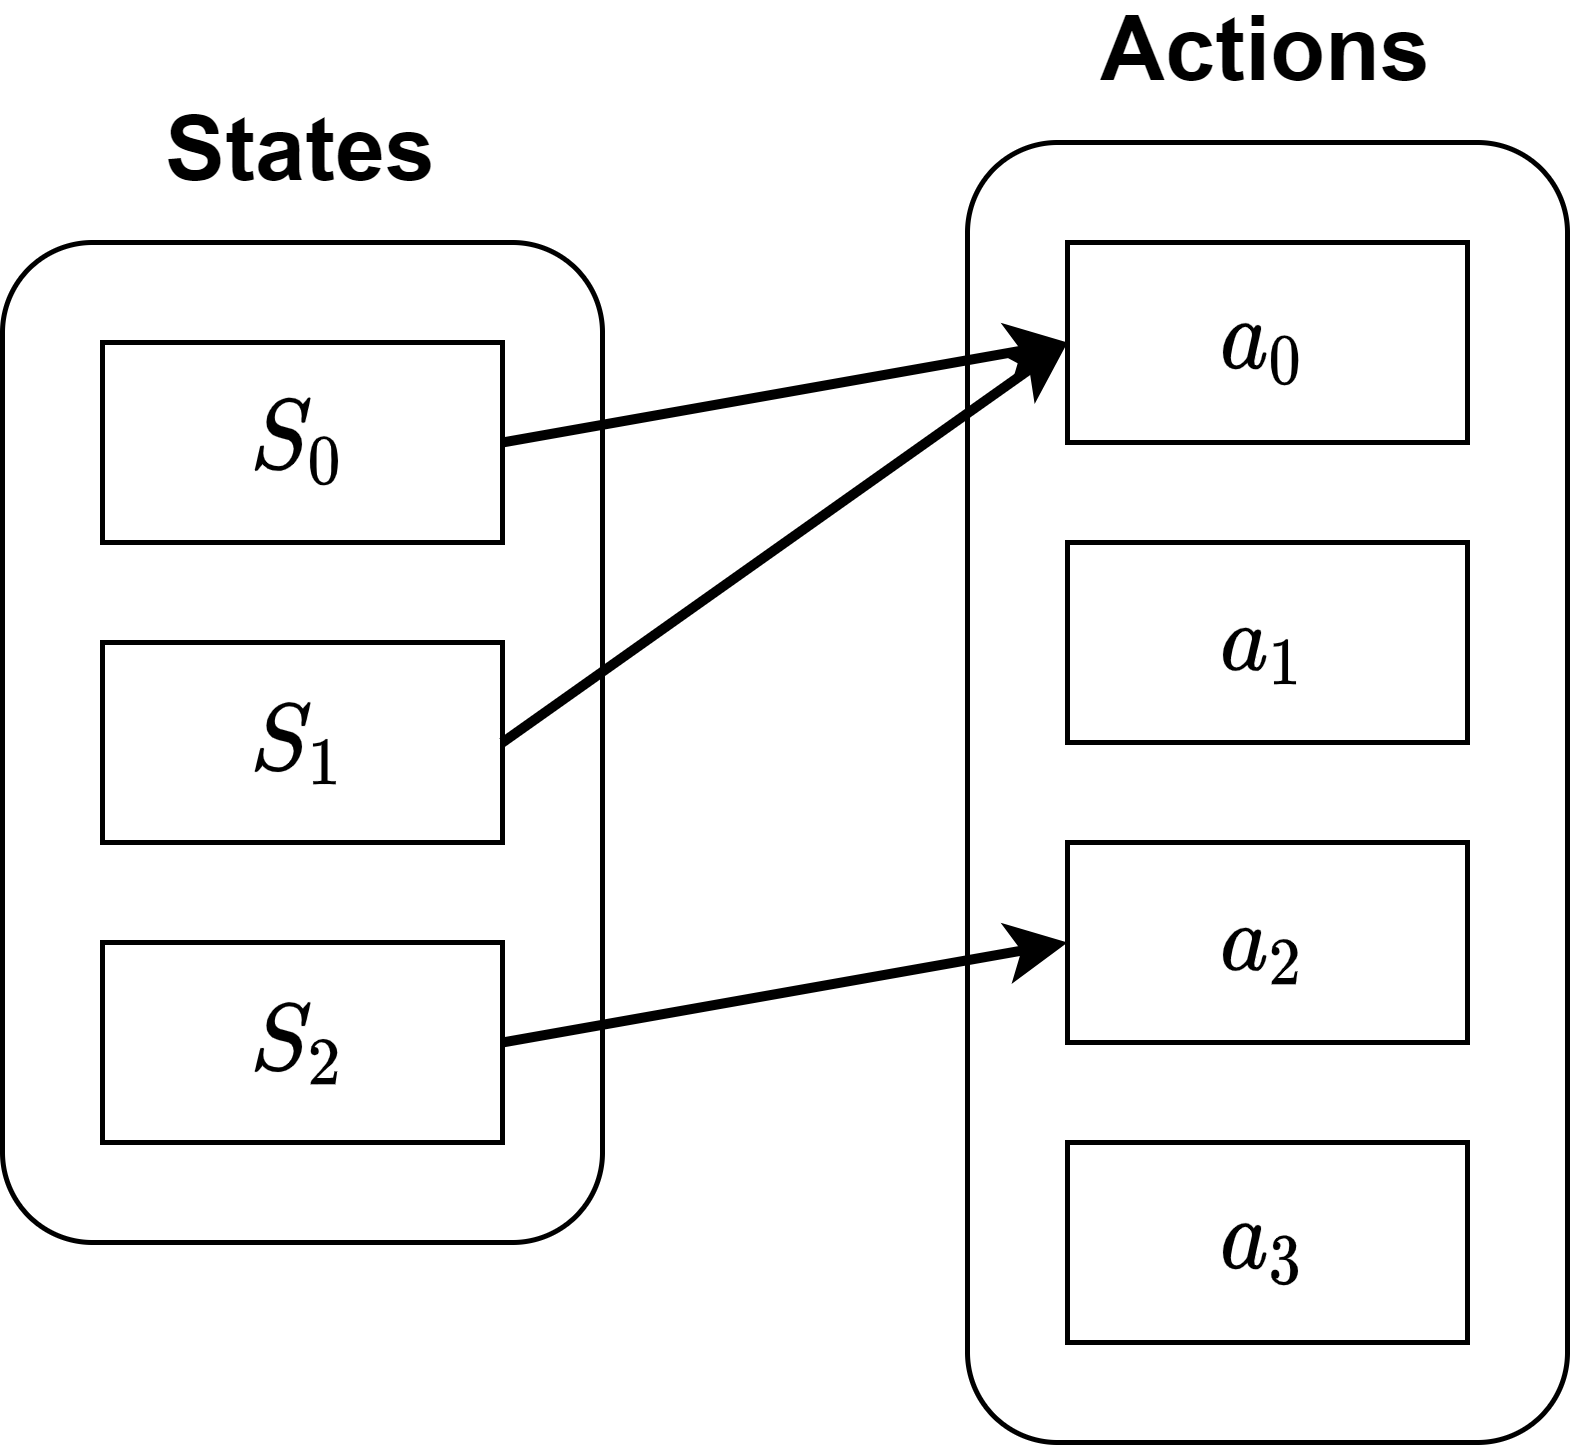
\includegraphics[width=0.95\textwidth]{Figures/Ch_MDP/deterministic_policy_drawio.png}
    \captionof{figure}{A deterministic policy behavior}
    \label{fig:MDP_deterministic_policy_example}
  \end{minipage}
  \hfill
  \begin{minipage}[b]{0.49\textwidth}
    \centering
    \begin{tabular}[b]{|c|c|}\hline
      State & Actions \\ \hline \hline
      $s_0$ & $a_0$ \\
      $s_1$ & $a_0$ \\
      $s_2$ & $a_2$ \\
      \hline
    \end{tabular}
    \captionof{table}{A deterministic policy behavior.}
    \label{tab:RNN-MDP_deterministic_policy_example}
    \end{minipage}
\end{minipage}

\begin{table}[h!]
\centering
\begin{tabular}{|c||c|c|c|c|}
\hline 
      & $a_0$ & $a_1$ & $a_2$ & $a_3$ \\ \hline \hline
\textbf{$S_0$} & \circled{\textcolor{red}{8.2}}   & -0.2  & 4.1   &  4.4 \\ \hline
\textbf{$S_1$} & \circled{\textcolor{red}{6.6}}   & -1.0  & -1.5  &  5.6 \\ \hline
\textbf{$S_2$} & -3.3  & -2.6  & \circled{\textcolor{red}{11.1}}  & -4.7  \\ \hline
\end{tabular}
\caption{Example of a Q-table}
\label{tab:MDP_Q_table}
\end{table}

\hspace{14pt}

Knowing the optimal $Q(s,a)$ function automatically gives us the optimal policy. Specifically, the best policy represents, at every state, choosing the optimal action:
\begin{align}
    \pi(s) = argmax_{a} \hspace{4pt} Q(s,a)
\end{align}

which provides the agent the optimal action based on the policy starting in the state ($s$) and all the way until the end of the episode. The policy ($\pi$ or sometimes $\pi(a|s)$), is a mapping from some state ($s$) to the probabilities of selecting each possible action given that state, as can be seen in Figure \ref{fig:MDP_deterministic_policy_example} and Table \ref{tab:MDP_Q_table}. For example, a greedy policy outputs for every state the action with the highest expected Q-Value.

\subsubsection{Q-Learning}
\label{subsubsec:MDP_Q_learning}

An ideal scenario would be that the value function is accurate in it's estimation of the true return from each state. However, a good value estimator needs to have good environment experience to learn from. 
To generate good experience trajectories, the agent needs to explore the environment and exploit the information it has learned.
Even with a branching factor of four (as shown in Figure \ref{fig:MDP_tree_structure}), the length of the tree can be massive both due to the length of the episode and the looping characteristics of the MDP. As such the agent needs to identify whether a tree node is good or bad and improve the value function estimate of only those nodes which are potential for optimal geometries. To satisfy both these requirements, we have to use Q-learning. Q-learning (QL) uses the information from the Value function along with a stochastic action to balance the dilemma of exploration and exploitation. This stochastic rule is called the $\epsilon$-greedy approach. 

\begin{figure}[h!]
    \centering
    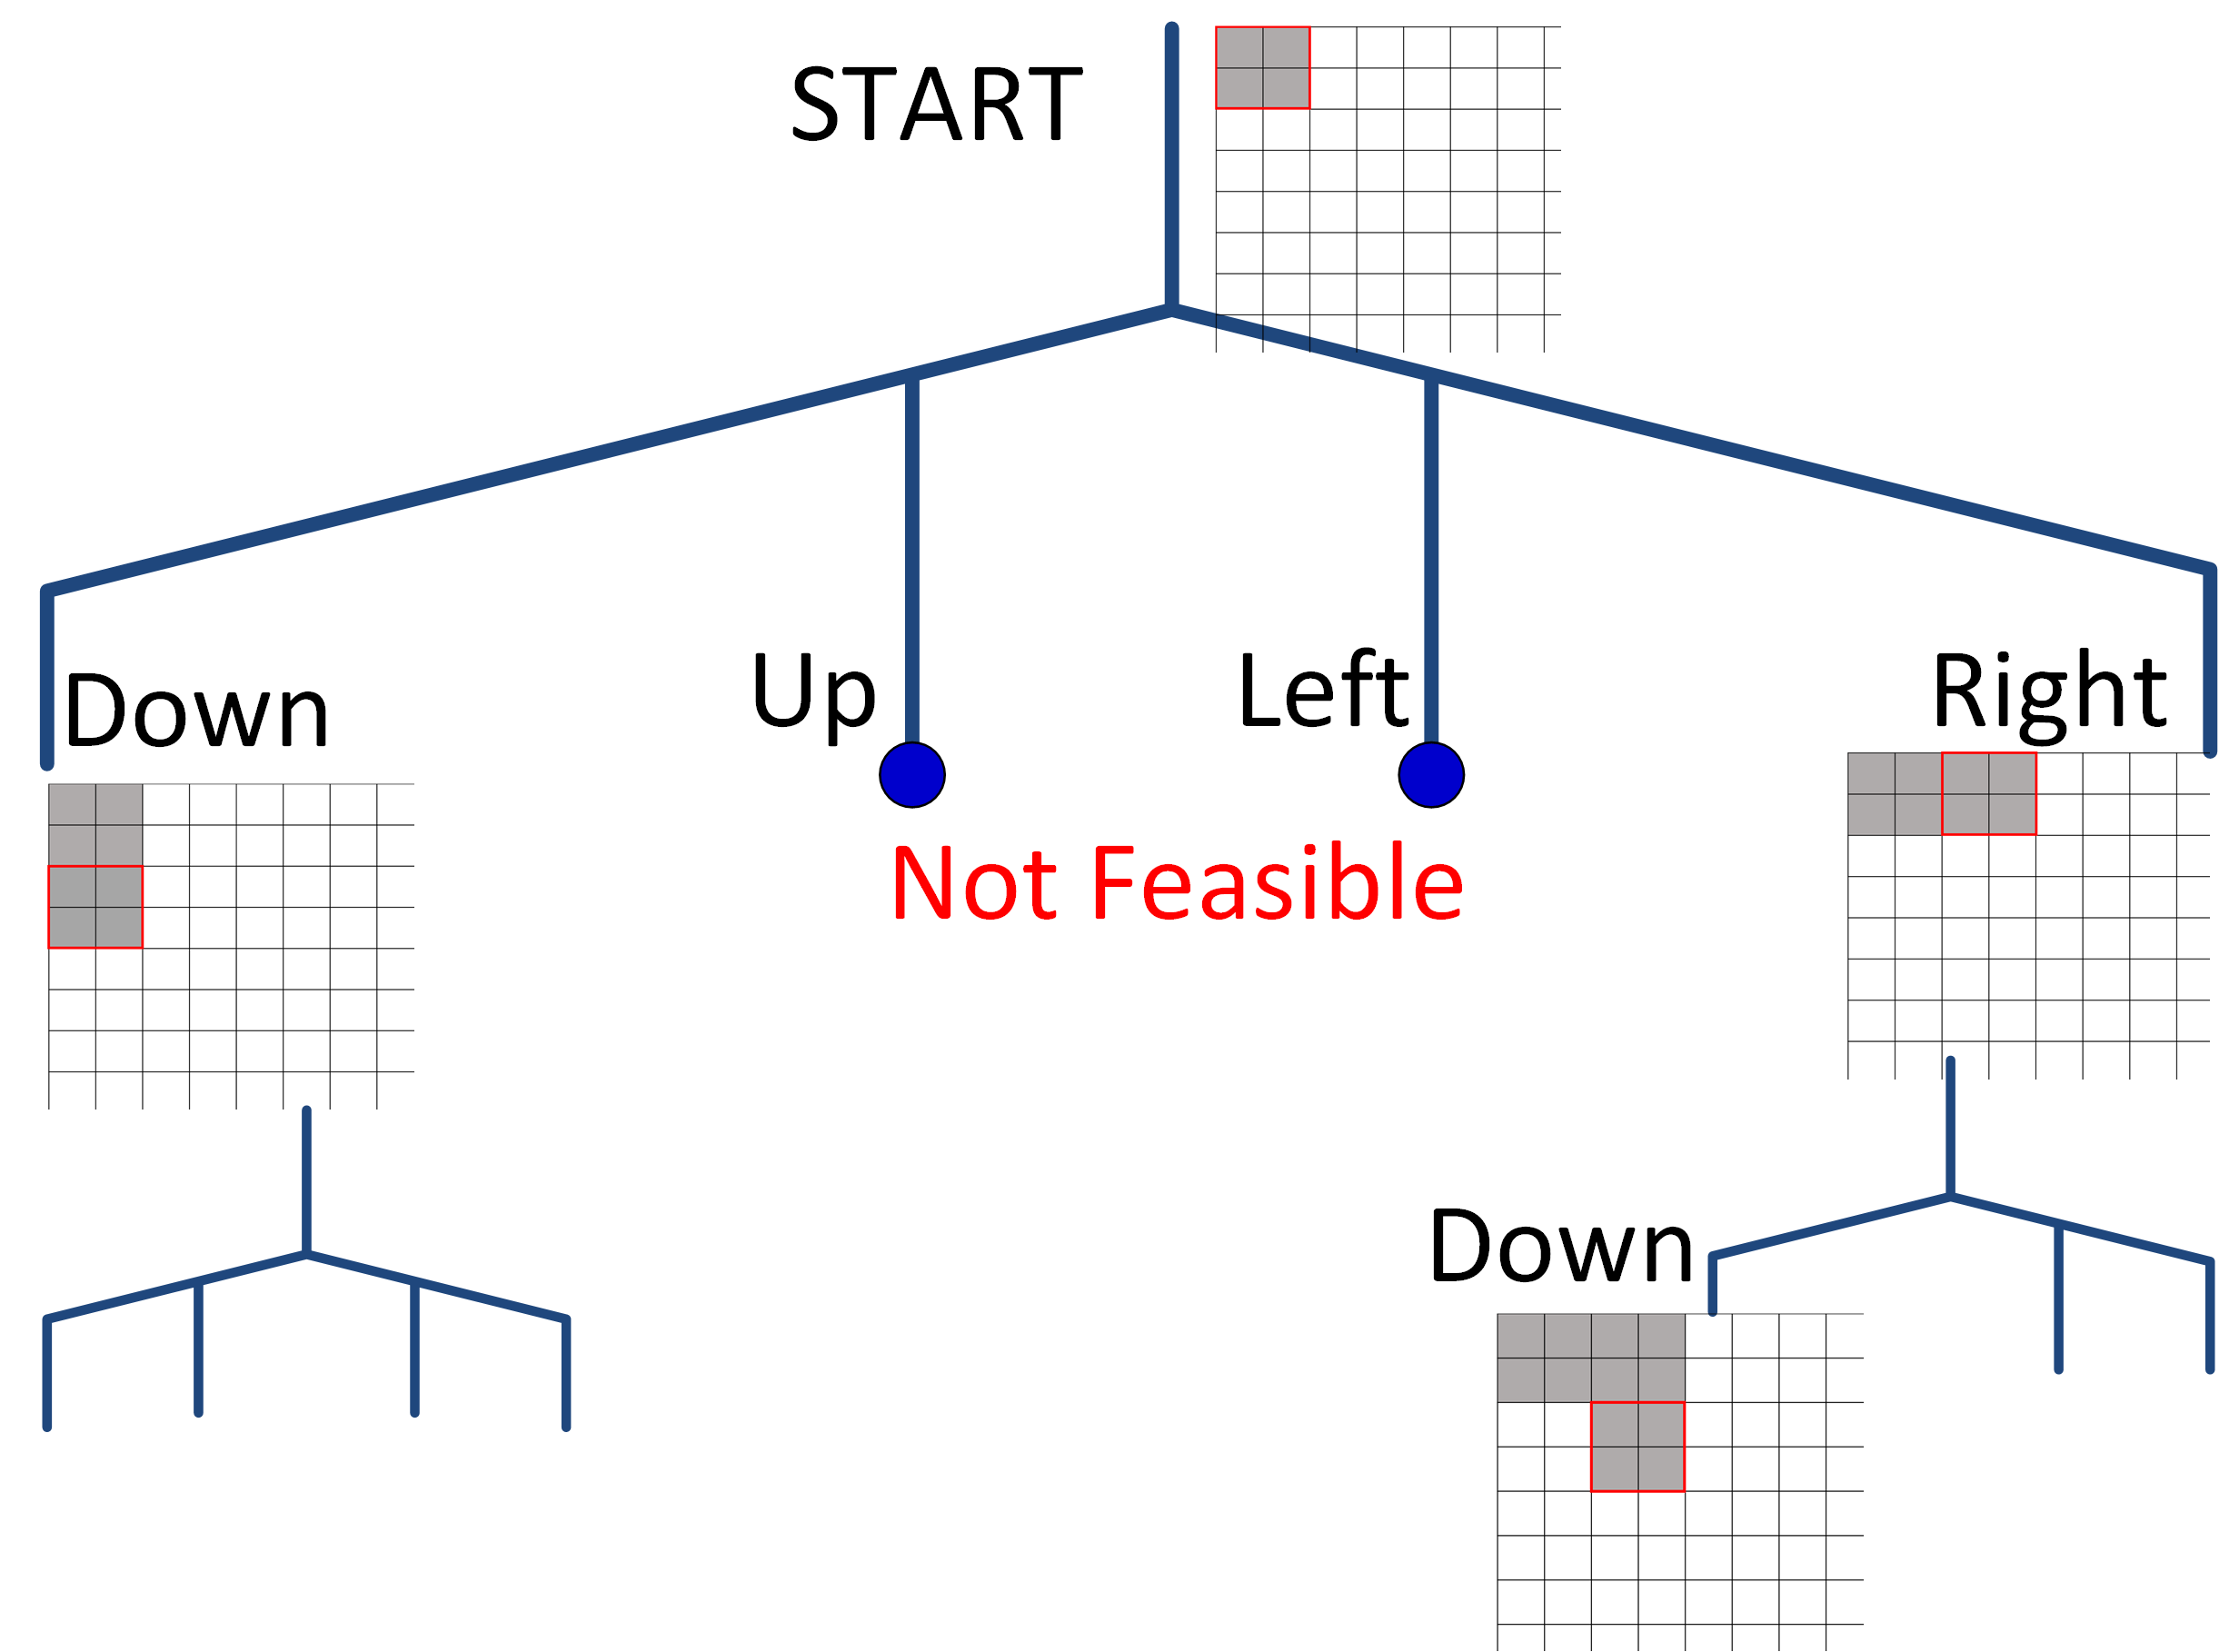
\includegraphics[width=0.50\textwidth]{Figures/Ch_MDP/Tree_structure.png}
    \caption{The tree diagram for the sequence based controller.}
    \label{fig:MDP_tree_structure}
\end{figure}

QL was developed in 1989 \parencite{watkins1992q}. It is one of the major online learning algorithms. The equation shown below describes the TD-learning based update rule for an Action value function (Q-function) 

It describes how the action values can be estimated incrementally
\begin{align}
    Q(s_t, a_t) \leftarrow Q(s_t, a_t) + \underbrace{\alpha}_\text{lr} \Big[ \overbrace{R_{t+1} + \underbrace{\gamma}_\text{df} \hspace{4pt} \underbrace{\underset{a'}{max} \hspace{2pt} Q(s_{t+1}, a')}_\text{off-policy}}^\text{TD-target} - Q(s_t, a_t) \Big]
\end{align}

The error in the estimate is the difference between the old estimate and the new target. Taking a step towards the new target will create a new estimate that reduces the error. The size of the step is determined by the step-size parameter called the `learning rate'. The value of step size is in the range of 0 and 1.

\subsubsection{$\epsilon$-greedy exploration}
$\epsilon$-greedy is a method for balancing the exploration and exploitation performed by the QL-based controller. Exploration allows the agent to improve its knowledge about each action. By improving the accuracy of the estimated action values, the agent can make more informed decisions in the future. Exploitation on the other hand exploits the agent's current estimated values ($Q(s, a)$). It chooses the greedy action to try to get the most reward. When the agent explores, it gets a more accurate estimate of its value function. On the other hand, when the agent exploits, it has a higher chance of getting more reward. It is not possible to choose both simultaneously. A simple method for choosing between exploration and exploitation is called $\epsilon$-greedy, which is a random process. 
This approach is based on a parameter $\epsilon$ which refers to the agent's probability of choosing to explore over exploit.
\begin{align}
    A_t  = 
    \begin{cases}
        \underset{a}{\arg\max} \; Q_t(s, a) \quad & \text{with probability} \; 1- \epsilon \\
        a \sim \uniform (a_1, \hdots a_k) \quad & \text{with probability} \; \epsilon
    \end{cases}
\end{align}

The action that is selected at time-step `$t$' is the greedy action with probability $1 - \epsilon$ or is a random action with probability $\epsilon$.
The value of $epsilon$ varies from 0 to 1. We usually start with a high $\epsilon$ value, close to 1. The higher the value of $\epsilon$, the more exploration the agent will perform as compared to exploitation. This can be justified during the initial stage of learning as the agent is new to the environment and cannot rely on a randomly initialized value function for exploitation. It needs to collect experience to train the value function and as the value function starts gaining capability, we reduce the exploration by decreasing the value of $\epsilon$. By the end of the training, $\epsilon$ decreases and goes down to a very low value of say 0.05. This makes sure that at any given point the agent will have some component of exploration. Once the agent converges to a policy that is not changing, the training stops. The starting value, decay rate, and stopping value of the $\epsilon$ are treated as hyperparameters in this study. In MDPs, there is always an optimal deterministic policy. In other words, you can always find a deterministic policy that is better than any other policy.

\subsubsection{Exploration - exploitation trade-off}
Pure greedy action selection can lead to sub-optimal behavior. Since the greedy action is always the same, the agent misses out on learning from the samples of alternative state action pairs. This induces the exploration-exploitation dilemma. It is important that the agent gets the chance to explore most (if not all) of the possible state-action pair that are there in the environment. However, this is an issue if the state space is of very high dimensionality. Further, for an MDP representation which involves the field value in the state representation (Figure \ref{fig:MDP_state_repr_2} \& \ref{fig:MDP_state_repr_3_Bfield}), a tabular method will fail. For a high dimensionality state-space or cases involving continuous values like the magnetic field distribution, one needs a function approximator that can handle this, which will be discussed in Chapter \ref{chapter:5_RL}.

\section{C-core - Topology Optimization Results} \label{sec:MDP_C_core_Topology_Optimization_Results}

\subsection{GA with SeqTO-\textit{v1}}

Different environments are set up based on the controller size (1 and 3), the type of material (linear: pure iron (linear B-H characteristics) and nonlinear: electrical steel (M-19 26 Ga)), the number of variables ($m$) and the population size (in multiples of $m$). The coil current is fixed at $1 A$ and the number of coil turns is set to 500. For this combination of coil turns and current, the force experienced by the armature of a conventional C-core EM actuator is $40 \hspace{4pt} N$, as shown in Figure \ref{fig:MDP_c_core_conventional_latex}, while the force (on the armature) obtained with an ON/OFF based TO algorithm in \parencite{midha2019selection, park2009} employing electrical steel is $50.90 \hspace{4pt} N$. This armature force decreases to $50.60 \hspace{4pt} N$ on application of post-processing filters to enforce topology smoothness \parencite{midha2019selection}.

\begin{figure}[h!]
    \centering
    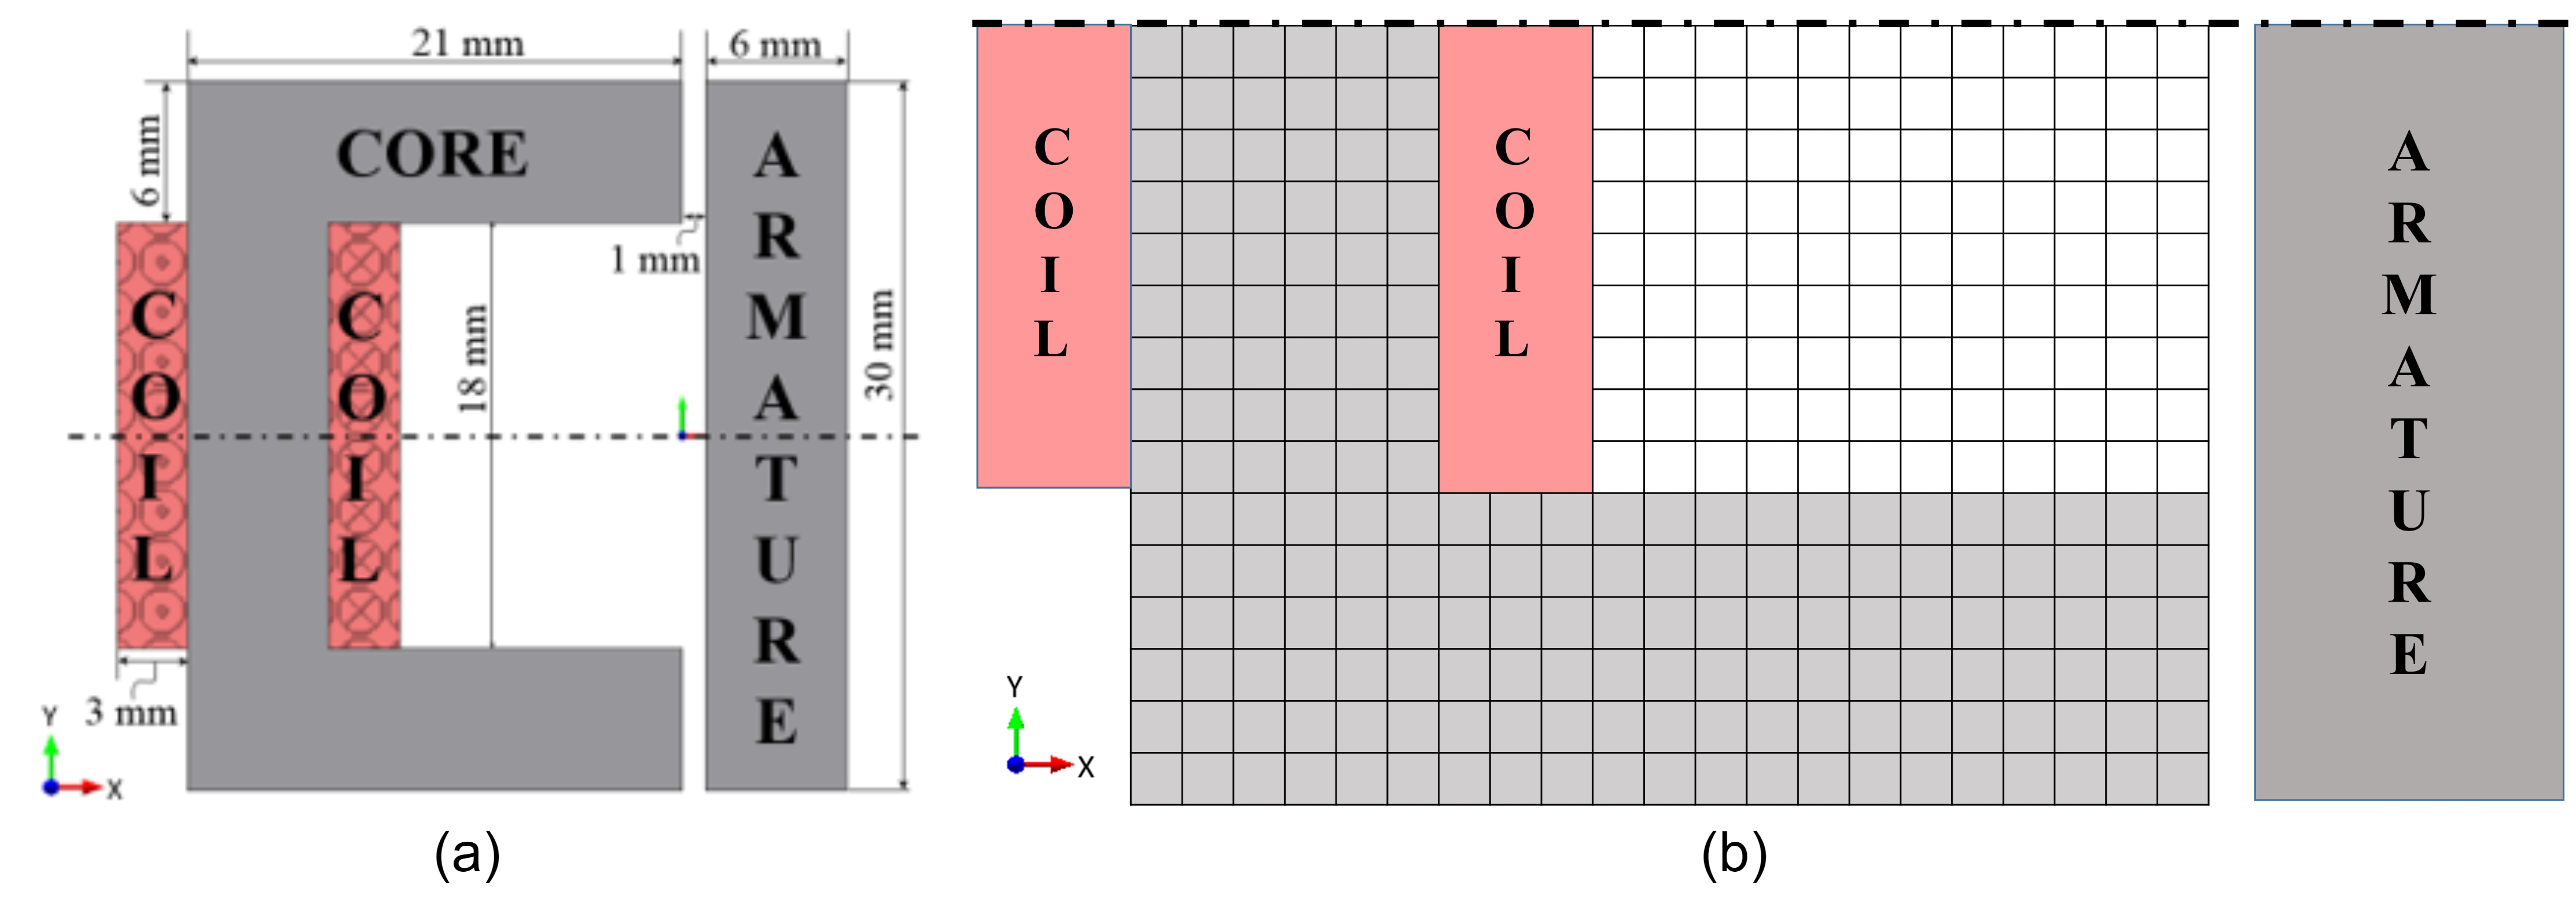
\includegraphics[width=\textwidth]{Figures/Ch_RL/c_core_conventional_latex.png}
    \caption{(a) Conventional C-core design (b) Only half of the geometry is simulated due to symmetricity.}
    \label{fig:MDP_c_core_conventional_latex}
\end{figure}


% Please add the following required packages to your document preamble:
% \usepackage{graphicx}
\begin{table}[h!]
\centering
\resizebox{\textwidth}{!}{%
\begin{tabular}{|c|c|c|c|c|c|}
\hline
\textbf{\begin{tabular}[c]{@{}c@{}}Environment \\ Type\end{tabular}} 
& \textbf{\begin{tabular}[c]{@{}c@{}}Design \\ Variables \\ (m)\end{tabular}} 
& \textbf{Pop. Size} 
& \textbf{\begin{tabular}[c]{@{}c@{}}Stall\\ Gen.\end{tabular}} 
& \textbf{\begin{tabular}[c]{@{}c@{}}Force\\ GA \\ {\footnotesize SeqTO-\textit{v1}}\end{tabular}}
& \textbf{\begin{tabular}[c]{@{}c@{}}Force\\ {\footnotesize GA On/Off} \\ {\tiny (\citeauthor*{midha2019selection})}\end{tabular}}
\\ 
\hline \hline
3 $\times$ 3 (Linear)            & 20                                                                                & 20 \| 40 \| 60          & 25                        & 70 N                 &     -                                          \\ \hline
3 $\times$ 3 (Linear)              & 25                                                                                & 25 \| 50 \| 75          & 25                        & 70 N                 &    -                                          \\ \hline
3 $\times$ 3 (Non-Linear)          & 30                                                                                & 20 \| 40 \| 60          & 25                        & 51 N                 &     -                                          \\ \hline
1 $\times$ 1 (Linear)              & 200                                                                               & 200               & 100                       & 71 N                   &        70 N                                     \\ \hline
1 $\times$ 1 (Non-Linear)          & 200                                                                               & 200               & 100                       & 55 N                     &      50.6 N                                      \\ \hline
\end{tabular}%
}
\caption{C-core results obtained from Genetic Algorithm using the SeqTO-\textit{v1} TO environment, along with a comparison of armature force wrt GA optimized results + filters \parencite{midha2019selection}.}
\label{tab:c_core_results}
\end{table}

Table \ref{tab:c_core_results} lists all the different case studies with the dimensions ($1 \times 1$ \& $3 \times 3$) referred to the size of the controller, along with the type of material used in the design space. The dimensionality of the controller is reflected in deciding the value of design variables ($m$) for GA \parencite{matlab} \parencite{GAtoolbox}. A limit on the number of stalled generations is employed to test for convergence. The initial population of the GA is based on a random seeding.

\begin{figure}[h!]
    \centering
    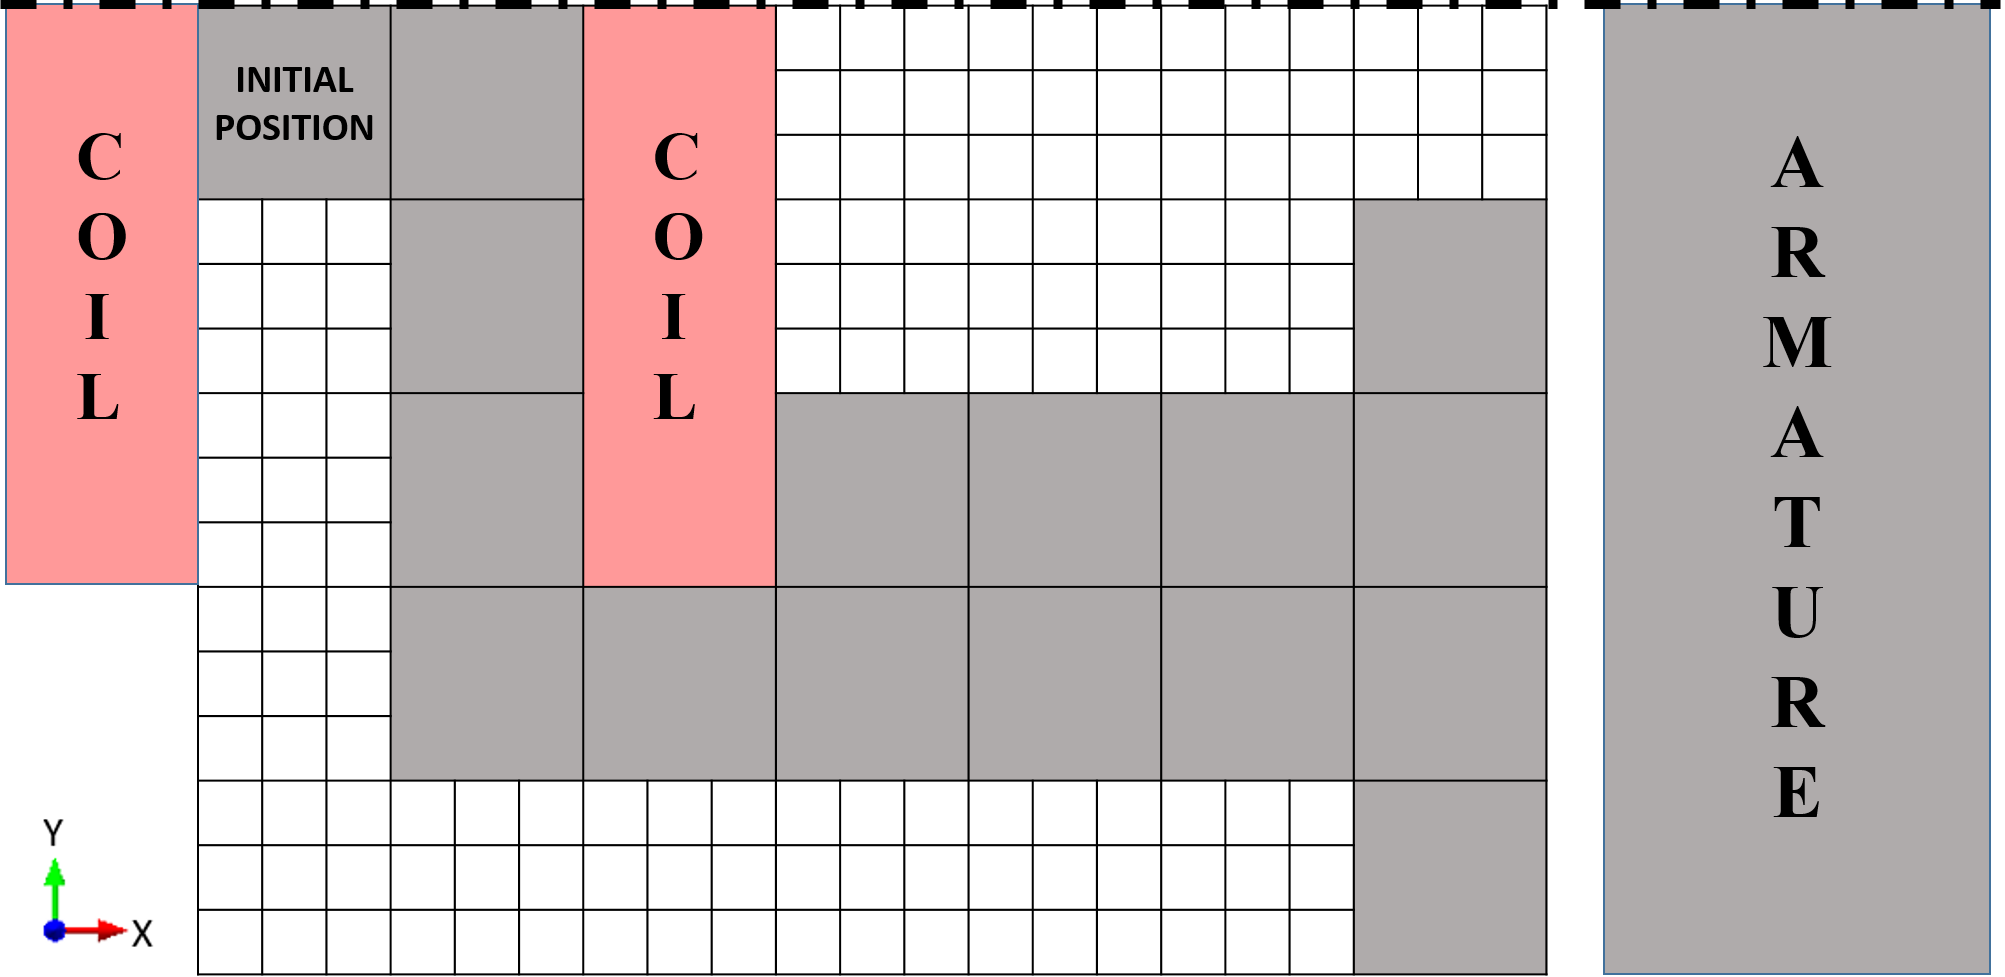
\includegraphics[width=0.75\textwidth]{Figures/Ch_MDP/C-Core_3X3Final.png}
    \caption{Optimized geometry for $3\times3$ Linear environment (SeqTO-\textit{v1} with GA).}
    \label{fig:MDP_3X3_linear_geometry}
\end{figure}

\begin{figure}[h!]
    \centering
    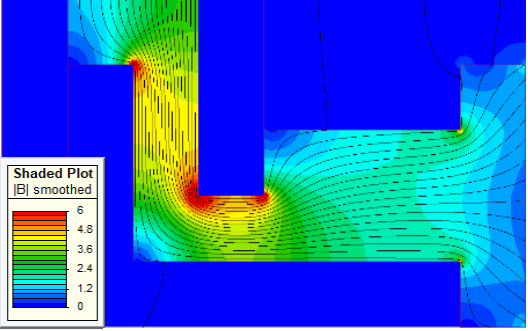
\includegraphics[width=0.75\textwidth]{Figures/Ch_MDP/state_repr_3_Bfield2.png}
    \caption{Optimized geometry's magnetic field distribution for $3\times3$ Linear environment (SeqTO-\textit{v1} with GA).}
    \label{fig:MDP_3X3_linear_Bfields}
\end{figure}

\begin{figure}[h!]
    \centering
    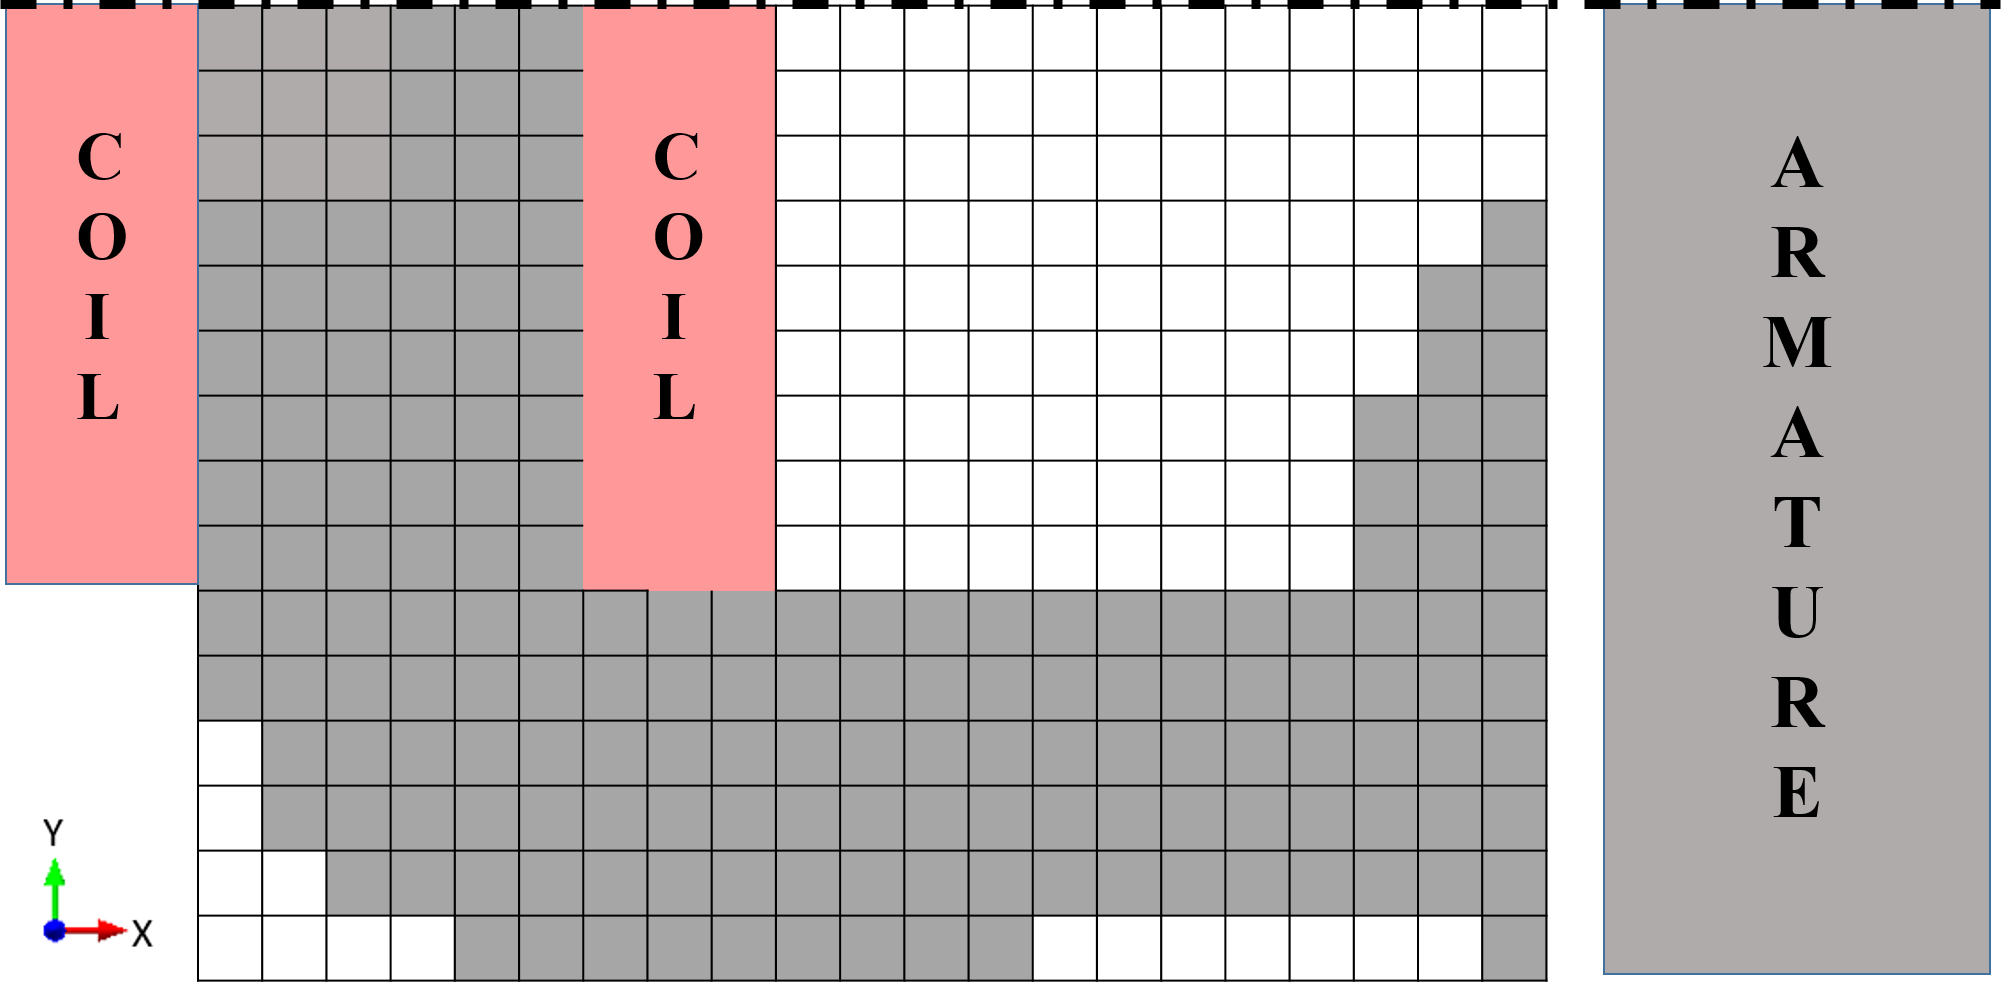
\includegraphics[width=0.75\textwidth]{Figures/Ch_MDP/C_core_1X1_end.png}
    \caption{Optimized geometry for $1\times1$ Non-linear environment (SeqTO-\textit{v1} with GA).}
    \label{fig:MDP_1X1_nonlinear_geometry}
\end{figure}

\begin{figure}[h!]
    \centering
    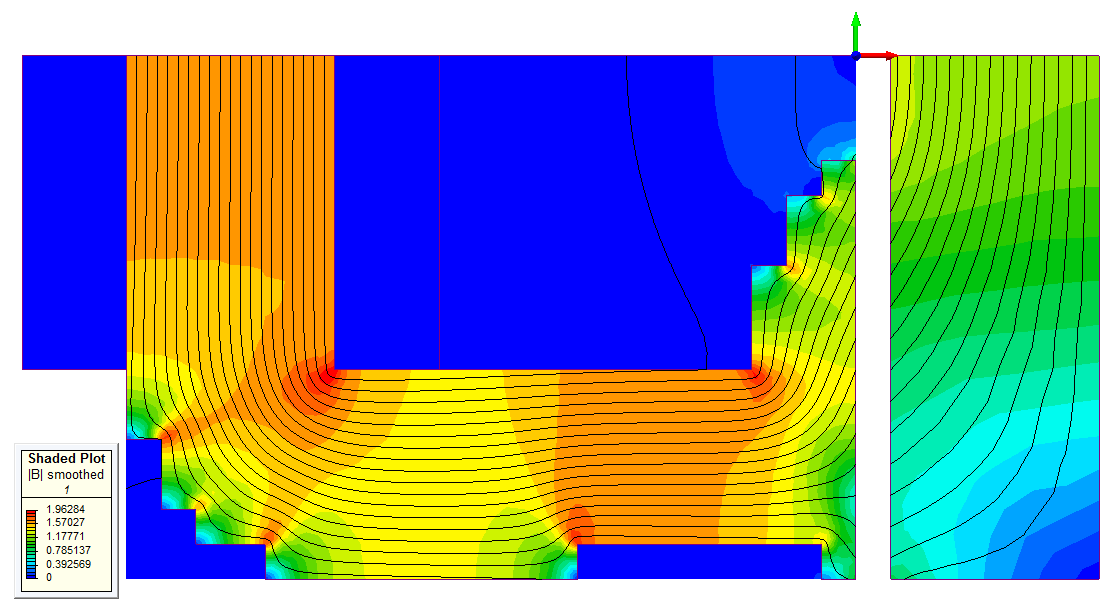
\includegraphics[width=0.75\textwidth]{Figures/Ch_MDP/55.8.png}
    \caption{Optimized geometry's magnetic field distribution for $1 \times 1$ Non-linear environment (SeqTO-\textit{v1} with GA).}
    \label{fig:MDP_1X1_nonlinear_Bfields}
\end{figure}

Using the setup discussed in Section \ref{section:set_seq_c_core}, GA is employed on SeqTO-\textit{v1} environment for all the case studies and the optimal force values are listed in Table \ref{tab:c_core_results}. It is observed that the bigger the size of the controller, the fewer the steps required to fill the design space. However, this affects the granularity of the optimal structure obtained, as can be seen through a comparison between a controller of size $3 \times 3$ (Figure \ref{fig:MDP_3X3_linear_geometry}) and $1 \times 1$ (Figure \ref{fig:MDP_1X1_nonlinear_geometry})  when the material of the controller is electrical steel. With the finer granularity controller ($1 \times 1$), GA managed to achieve a higher performance value for the optimal design. The optimal design obtained using a $1 \times 1$ controller on SeqTO-\textit{v1} environment produced a force of $55 \hspace{4pt} N$, an increase of about 8\% as compared to using a controller of size $3 \times 3$ ($51 \hspace{4pt} N$). 


Finally, as it is evident from Table \ref{tab:c_core_results}, this new sequence based TO method performs on par with \cite{midha2019selection} (for the linear case: $70 \hspace{4pt} N$) and achieves a good increase in force when compared for the non-linear cases (8.7\% improvement).

\subsection{C-core: Results of TD-learning}

Based on the design setup in Section \ref{section:MDP_TD_learning}, a linear material based controller of size three is tested on the SeqTO-\textit{v1}. 
The optimal geometry for a $3 \times 3$ SeqTO-\textit{v1} environment with linear material is shown in Figure \ref{subfig:td_linear_action_seq}. This result matches the geometry obtained through the GA algorithm (Figure \ref{fig:MDP_3X3_linear_geometry}). In addition to the optimal geometry, we can get a sequence of actions that are greedy in nature, as proven by the monotonic increase in reward function in the graph (Figure \ref{subfig:td_linear_force_v_steps}) between the force acting on the armature and the step-index. This gives a greedy action that tries to continuously increase the value of the force both for the near future and for the final optimal geometry. The agent needs to account for the long-term impact of its actions. As such the agent creates a channel to feed magnetic flux lines in the armature. This leads to an increase in the magnitude of magnetic flux in the armature, which in turn increases the force value on the armature. However, this results in magnetic field saturation in the iron placed earlier by the agent. 
This poses a conundrum for the agent as to whether it should place material near the armature to increase the surface area near the airgap and feed more flux or go back and take care of the magnetic saturation in the core of the design.
Such information can be helpful in analyzing the importance of each element in the whole topology. Further, a designer can use this knowledge to understand the trade-off of any element with the performance and can further fine-tune the structure without running an optimization algorithm.

\begin{figure}[h!]
    \centering
    \begin{subfigure}{.45\textwidth}
        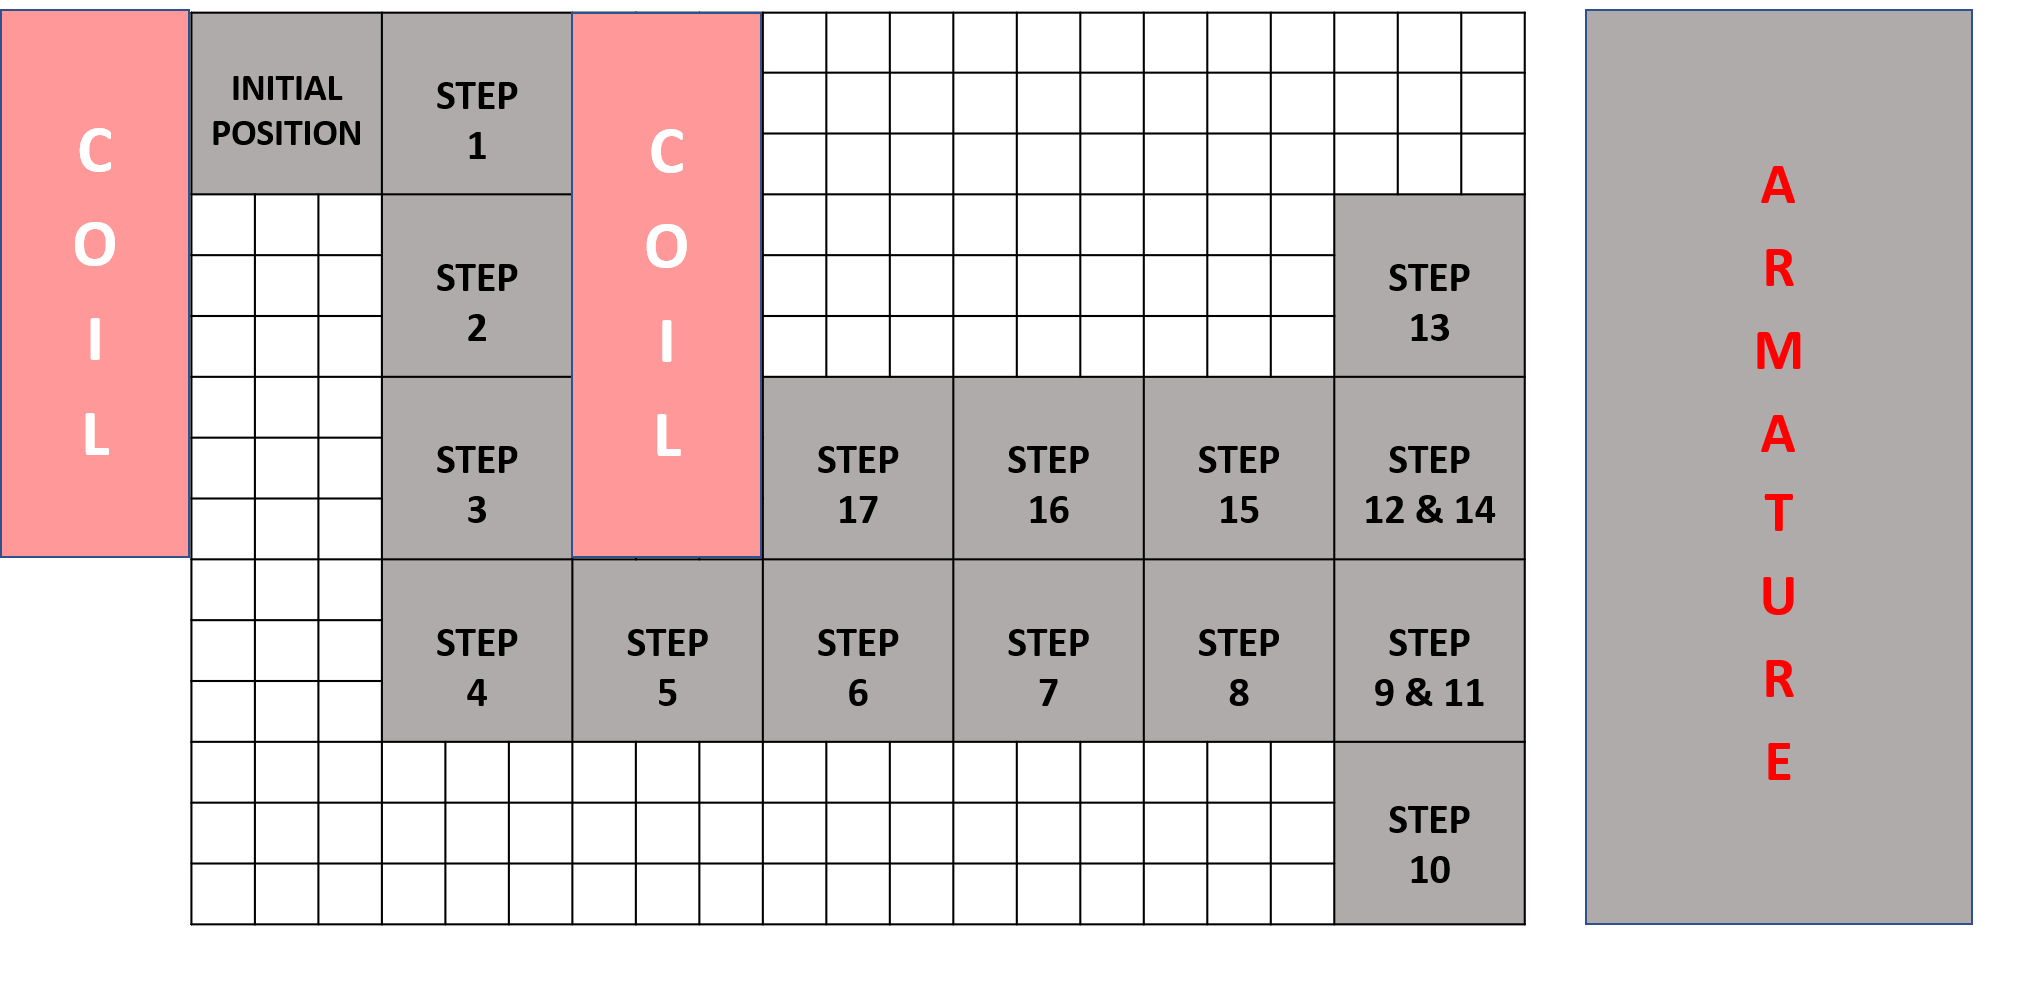
\includegraphics[width=\linewidth]{Figures/Ch_MDP/agent_result_TDlearning.png}
        \caption{The optimal solution and action sequence in a $3 \times 3$ linear environment}
        \label{subfig:td_linear_action_seq}  
    \end{subfigure}
    \begin{subfigure}{.45\textwidth}
        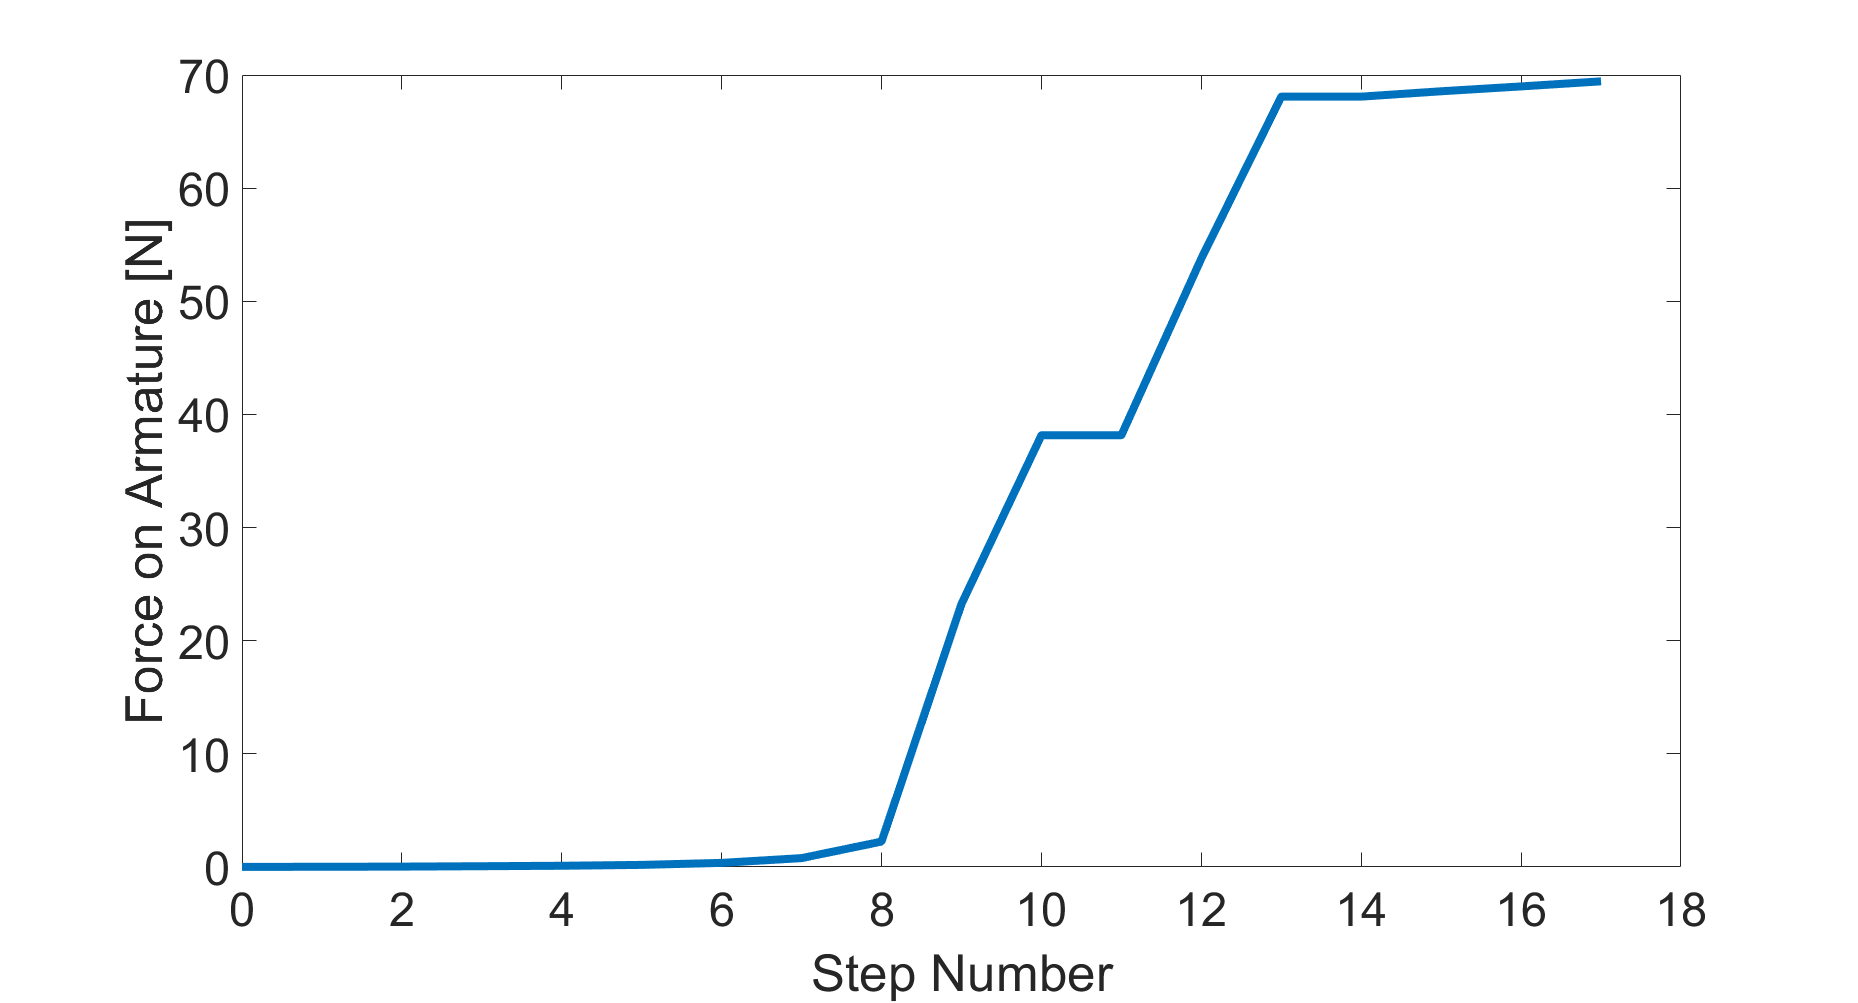
\includegraphics[width=\linewidth]{Figures/Ch_MDP/Force_arm_TD_lear.png}
        \caption{Force on armature vs steps in an episode}
        \label{subfig:td_linear_force_v_steps}  
    \end{subfigure}
    \caption{Optimal solution $3 \times 3$ controller (SeqTO-\textit{v1}) with TD-learning, on a C-core design domain.}
\end{figure}

\section{Synchronous Reluctance Motor}

Extending the SeqTO-\textit{v1} to more complex electric machines, the rotor of a Synchronous Reluctance Motor (SynRM) is optimized using the proposed TO methodology.

The industrial applications of SynRMs have risen in the past few decades, due to their simple structure and low costs. The SynRM offers a number of advantages. Some of them are listed here:

\begin{itemize}
    \item High efficiency
    \item High power density
    \item Less maintenance
    \item Reduced inertia
    \item Very Reliable
\end{itemize}

Compared to Induction Motors (IMs), which have been the industry standard for many decades, the SynRM can offer high power density for a smaller footprint. 
This can be almost 2 to 4 times higher than an IM, with a frame size almost 1-2 times smaller \parencite{ABB_driving_force_REE}. The SynRM is also one of the most efficient motors available to the industry, with a recent development even reporting an efficiency value as high as 99.05\% (full load on a 44 MW, 6 pole, synchronous motor) \parencite{ABB_record_99}. Such highly efficient motors are the future, especially when motors employed by the industries consume about 28-30\% of the world's electricity \parencite{kober2020global, IEA_WEO_2019}. Further, a SynRM also operates at a lower temperature as compared to an IM, helping with a longer operational life of insulation, bearing, etc. Internal bearing failure is a major concern with an IM, being responsible for almost 40 \% of IM failures \parencite[IEEE Survey]{IEEE_IM_survey}. In addition, with the absence of slip rings, rotor field windings. permanent magnets, commutators, and brushes, SynRMs have a low manufacturing cost, require less maintenance, and offer longer operation life. Some of their practical applications include usage in washing machines, analog electric meters, hard drives disks and electric vehicles.

\begin{figure}[h!]
    \centering
    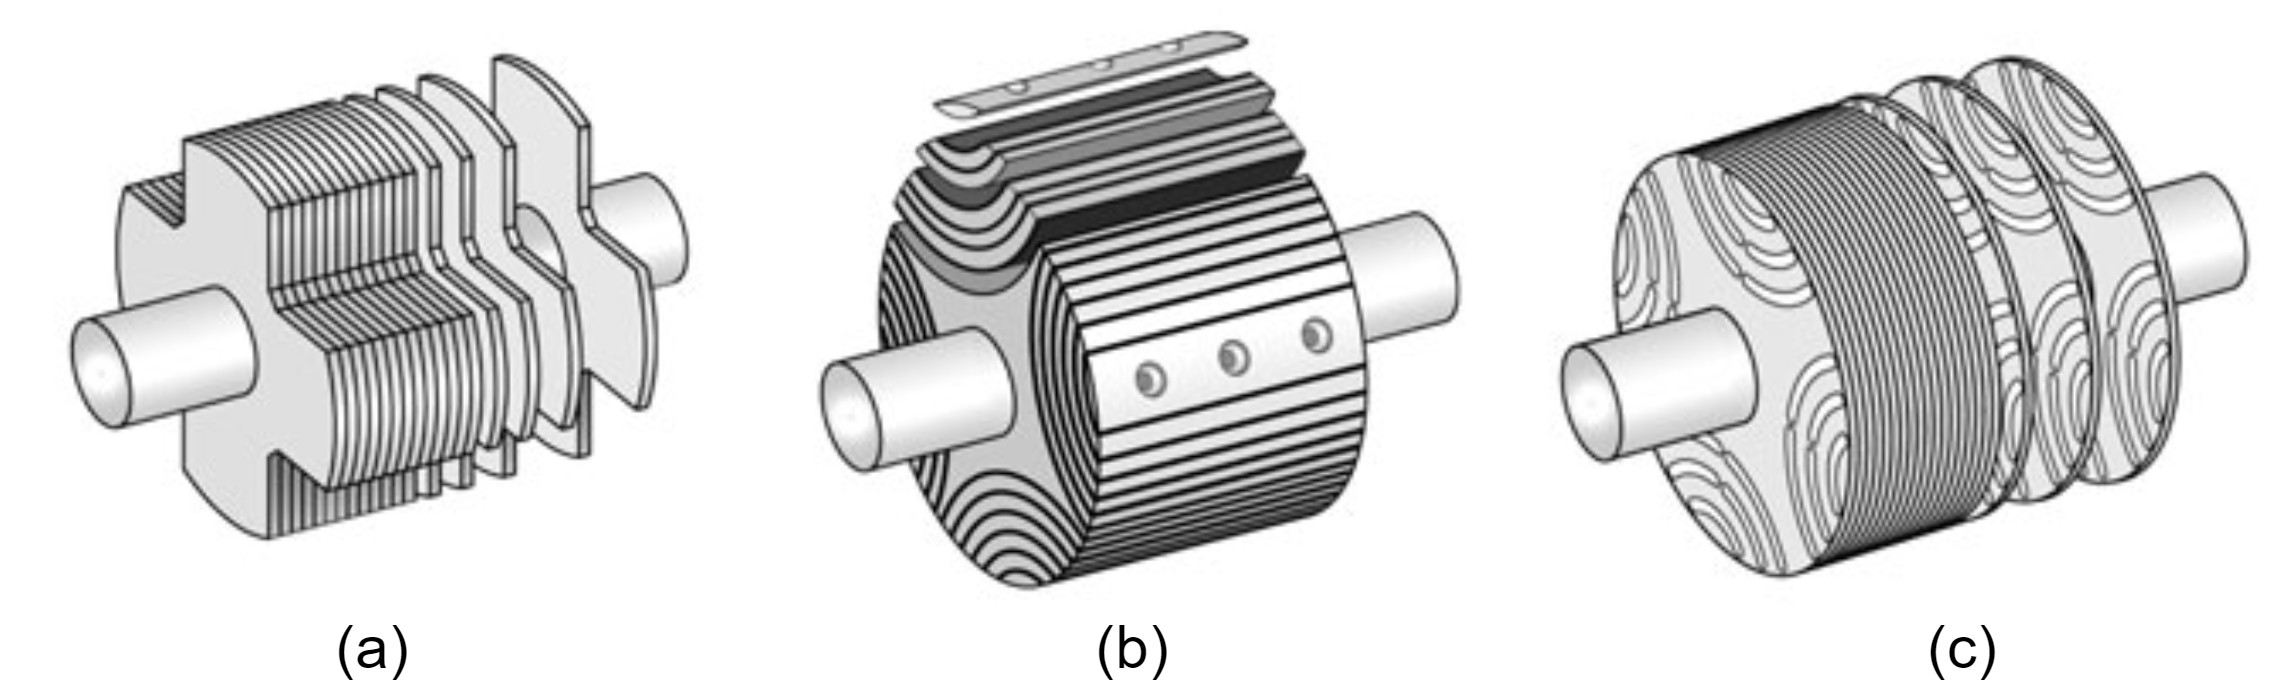
\includegraphics[width=0.85\textwidth]{Figures/Ch_MDP/reluctance_motor_rotor.png}
    \caption{Conventional rotor designs for synchronous reluctance motors (a) salient pole type, (b) axial lamination type (c) transverse lamination type \parencite{kolehmainen2010synchronous}.}
    \label{fig:MDP_SynRM_rotor_geo}
\end{figure}

Although reluctance-based machines were invented in the $19^{th}$ century, they have gained popularity only since the advancement of microelectronics and control systems.
SynRM operates at exact - ``synchronous" speed by syncing the rotor speed with the stator's rotating magnetic field.  
The rotating MMF in the stator can be generated by exciting a 3 phase stator winding. The rotor poles exhibit saliency due to internal magnetic barriers (slots, airgaps) or external notches. The presence of notches/barriers/slots in the rotor structure can affect the profile of the reluctance torque experienced by the rotor. The three types of synchronous reluctance rotors, as per the literature, are the simple salient pole rotor, the transverse laminated rotor, and the axially laminated rotor \parencite{kolehmainen2010synchronous}, as seen in Figure \ref{fig:MDP_SynRM_rotor_geo}. Due to the law of conservation of energy, the rotor will always try to move to a position of least reluctance with respect to the stator. With the help of proper and controlled excitation in the stator poles, the movement of the rotor will be continuous and at a fixed ``synchronous" speed. However, the average torque produced by a SynRM is still inferior when compared to other motors such as a permanent magnet motor \parencite{murakami1999performance} and is an active field of research \parencite{li2013multiobjective, hidaka2017topology, kim2010topology}. As a SynRM produces reluctance torque through a salient rotor structure, the rotor flux barriers play a vital role in the design optimization of SynRMs, since they force the main flux through the desired iron paths within a fixed stator geometry. Thus, to improve the performance of SynRM, it is important to optimize the shape of the barrier of the rotor of a SynRM. The objective will be similar to that in Section \ref{section:set_seq_c_core} and also stated in eqn. \ref{eqn:MDP_optimization_problem_formulation_SynRM}, where $f(a)$ is the negative magnitude of the average torque generated by the motor. The sequence of actions ($a$) controls the movement of the controller. 
However, the material distribution controlled by $a$ is air ($p_j: 1 \rightarrow 0$), resulting in a rotor's flux barrier.

\begin{align}
    \begin{split}
        \underset{\substack{a_i = {0, 1, 2, 3} \\ i = 0, 1, 2, \hdots, m}}{minimize} & \hspace{10pt} f(a) \\
        \text{subject to} \hspace{14pt} K1 \leq & \sum_{j=1}^n (p_j = 0) \leq K2 \label{eqn:MDP_optimization_problem_formulation_SynRM}
    \end{split}
\end{align}

\begin{figure}[h!]
    \centering
    \begin{subfigure}{0.3\textwidth}
        \centering
        
\includegraphics[width=\linewidth]{Figures/Ch_MDP/SynRM_dual_conventional_small.png}
        \caption{Conventional single barrier SynRM}
        \label{subfig:MDP_SynRM_dual_conventional}
    \end{subfigure}
    \begin{subfigure}{0.3\textwidth}
        \centering
        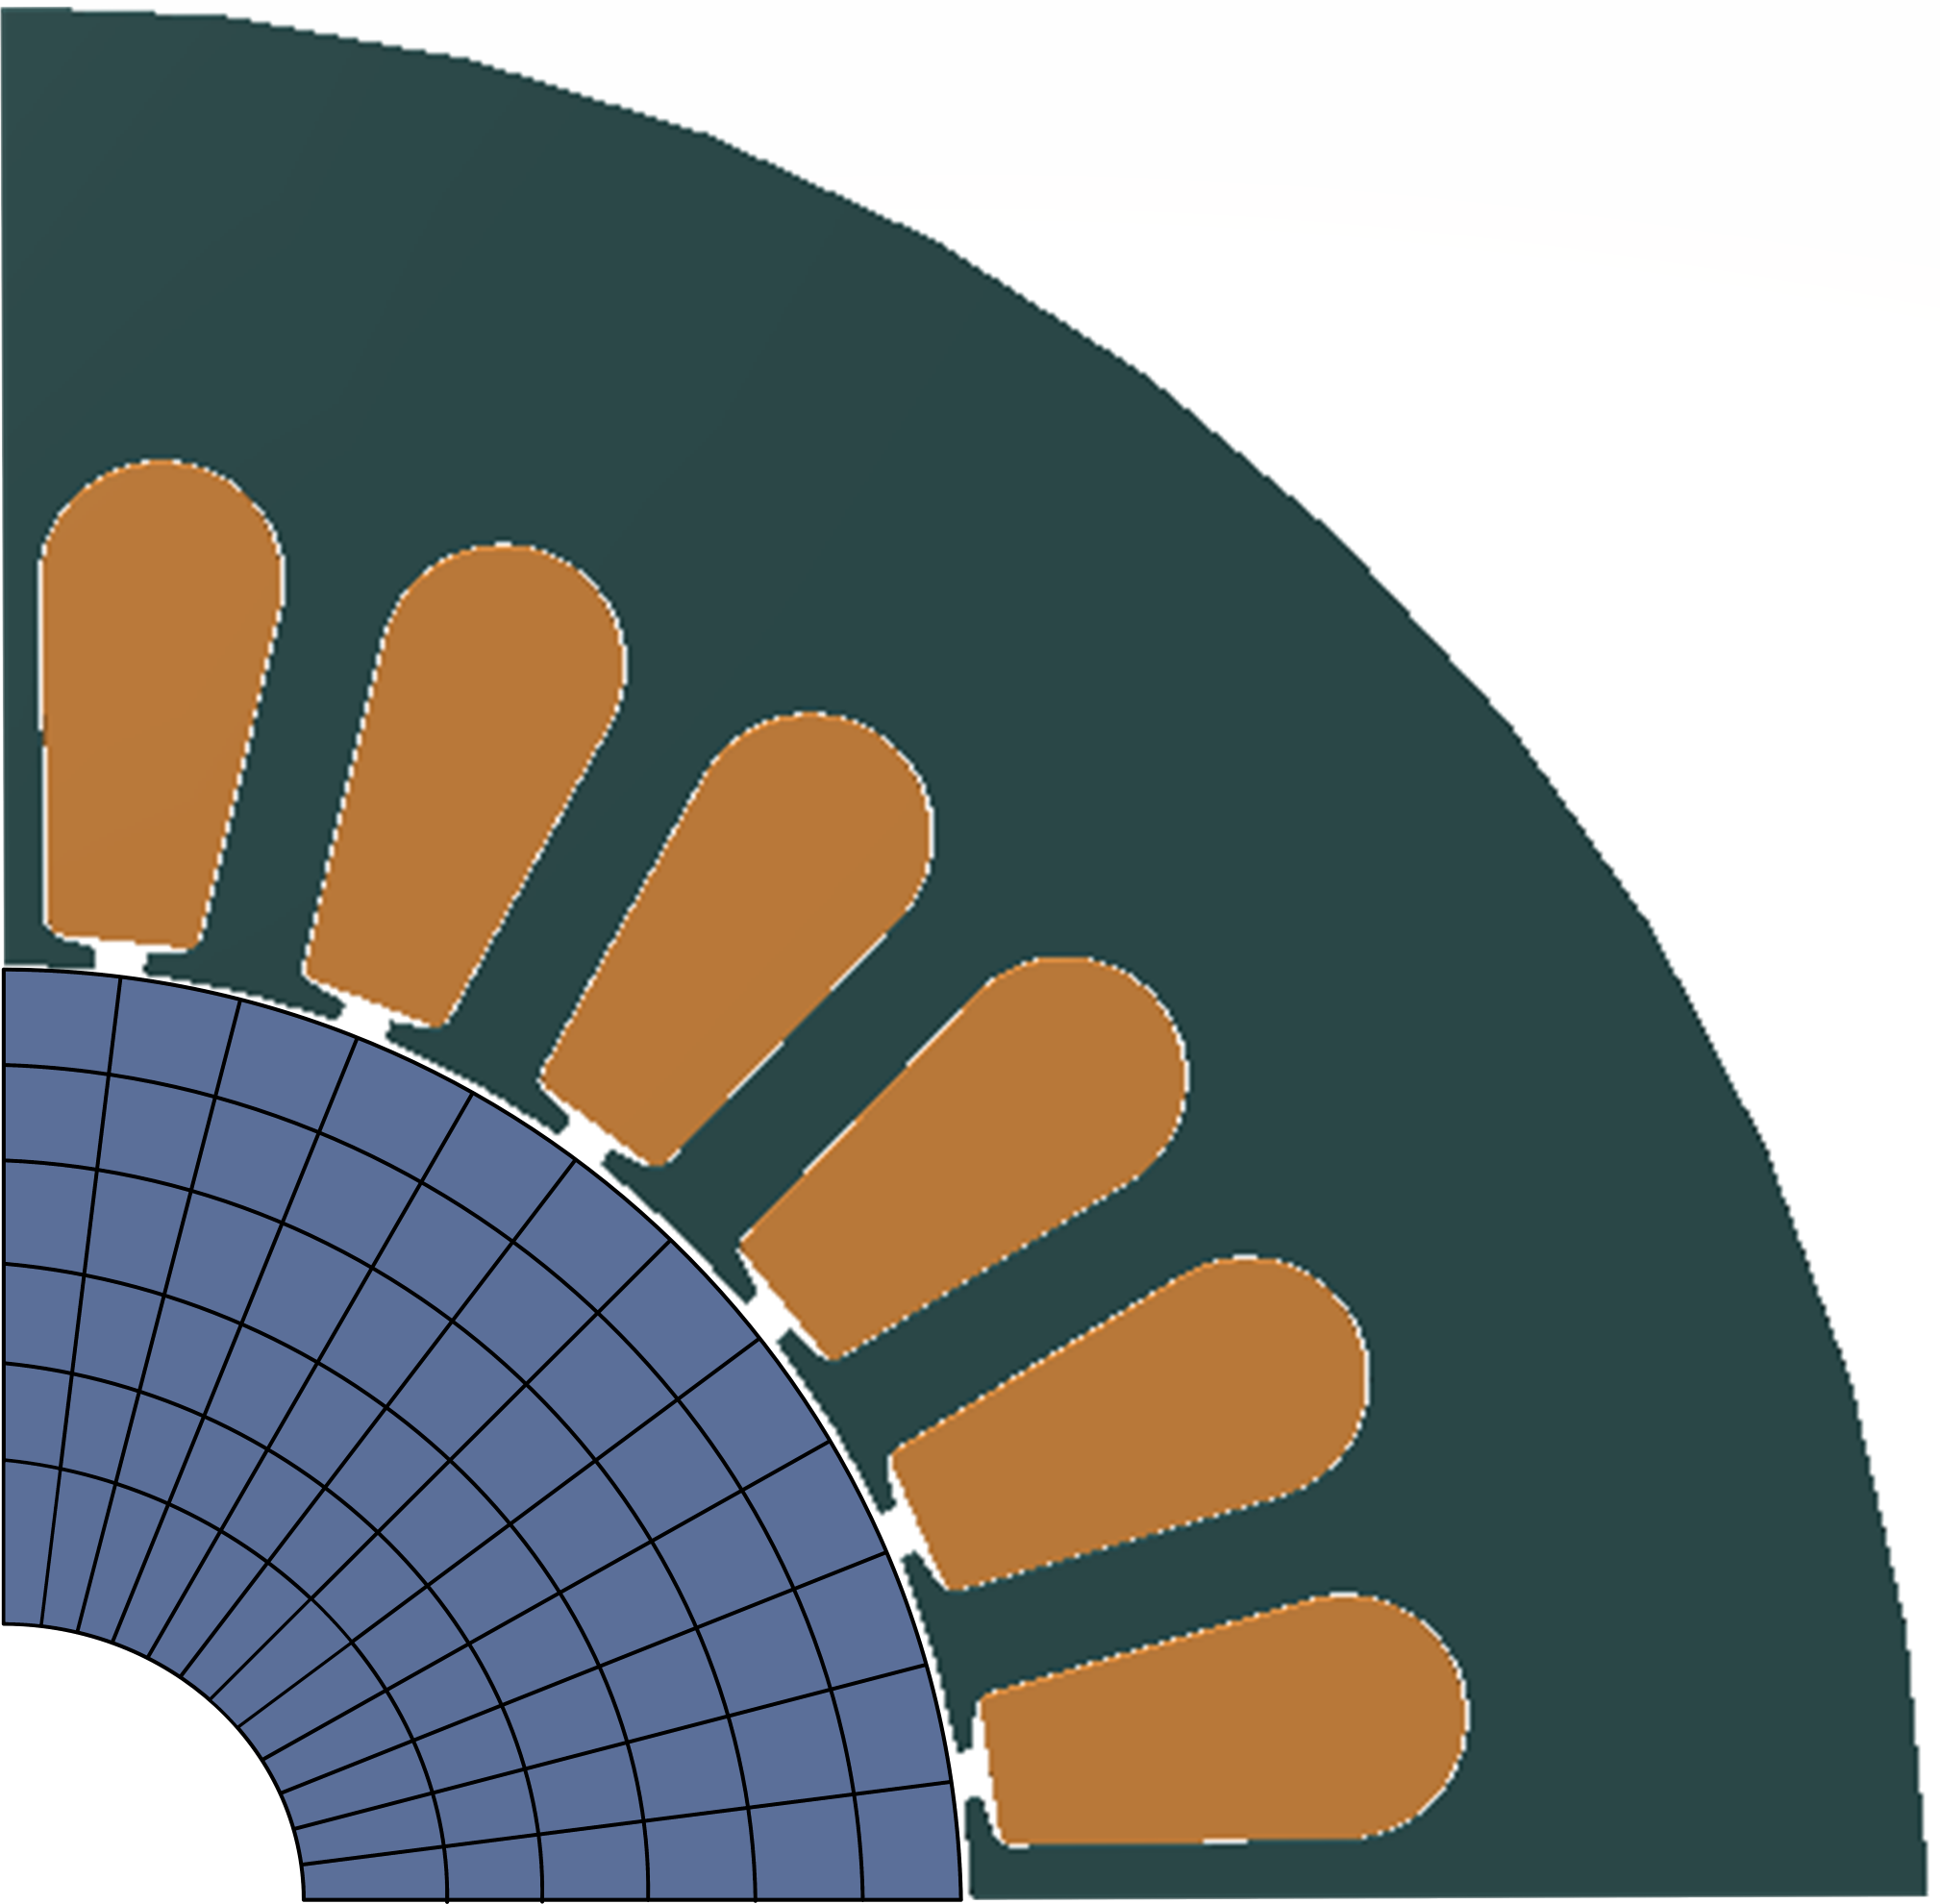
\includegraphics[width=\linewidth]{Figures/Ch_MDP/SynRM_dual_blank2_small.png}
        \caption{Discretized rotor geometry}
        \label{subfig:MDP_SynRM_dual_blank2}
    \end{subfigure}
    \begin{subfigure}{0.3\textwidth}
        \centering
        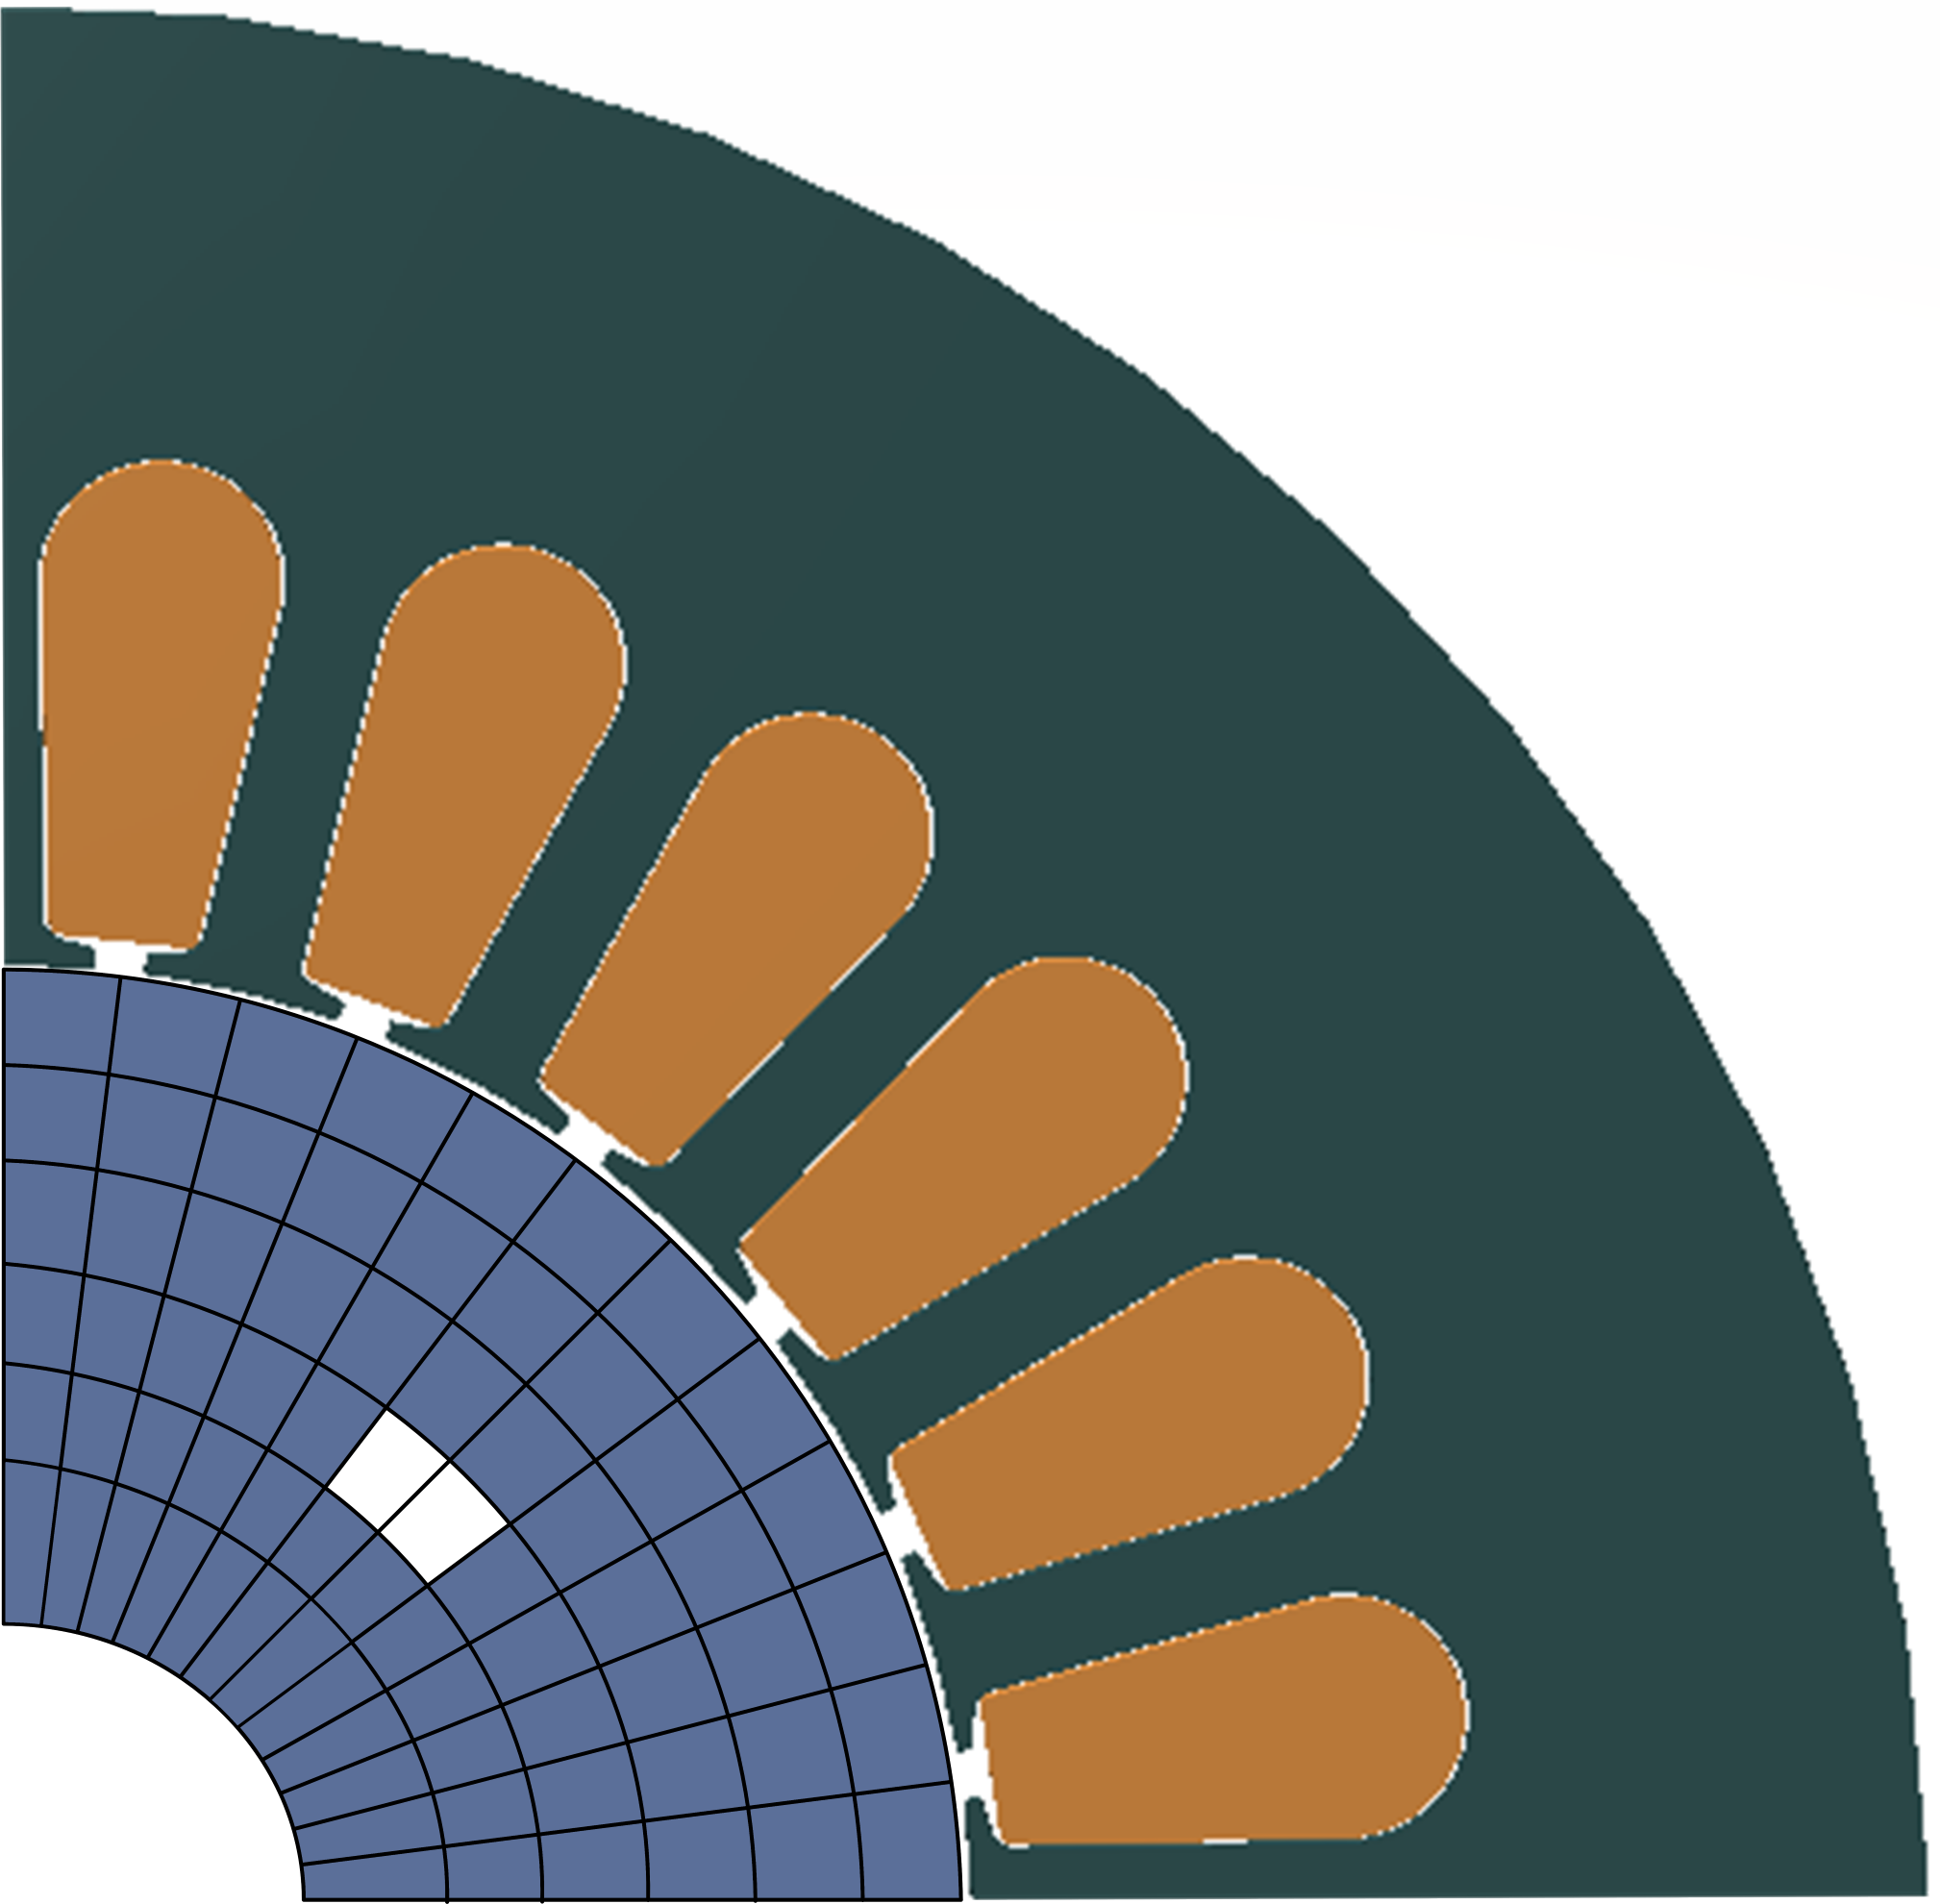
\includegraphics[width=\linewidth]{Figures/Ch_MDP/SynRM_dual_start2_small.png}
        \caption{Controller at start position.}
        \label{subfig:MDP_SynRM_dual_start2}
    \end{subfigure}
    \caption{SynRM characteristics}
    \label{fig:MDP_SynRM_characteristics}
\end{figure}

The definition of other parameters ($p,K1,K2$) associated with defining the problem remains the same as in Section \ref{section:set_seq_c_core}. The geometry for baseline performance was extracted from Siemens's MAGNET \parencite{Magnet}  with the fixed parameters mentioned in Table \ref{tab:MDP_synRM_fixed_parameters} and displayed in Figure \ref{subfig:MDP_SynRM_dual_conventional}. The baseline SynRM exhibits an average torque of 2.5 N-m. Taking advantage of the symmetry offered by a 4-pole, 3-phase design, only a quarter of the geometry is considered as the design space. The quarter 2-D design space is discretized into $25$ ($5 \times 5$) cells with the initial design filled with iron ($p_i=1$) and can switch to air ($p_i=0$), based on the movement of the controller. The cross-section of the discretized design space is shown in Figure \ref{subfig:MDP_SynRM_dual_blank2} and the starting position of the controller in Figure \ref{subfig:MDP_SynRM_dual_start2}.

% Please add the following required packages to your document preamble:
% \usepackage{graphicx}
\begin{table}[h!]
\centering
%\resizebox{\textwidth}{!}{%
\begin{tabular}{|c|c|c|c|}
\hline
\textbf{Fixed Parameters} & \textbf{Value} & \textbf{Fixed Parameter} & \textbf{Value} \\ \hline \hline
Number of stator slots    & 24             & Number of Poles          & 4              \\ \hline
Stator outer diameter     & 112 mm         & Airgap thickness         & 0.5 mm         \\ \hline
Rotor outer diameter      & 55 mm          & Stack height             & 50 mm          \\ \hline
Rotor inner diameter      & 16 mm          & RMS current density      & 18 A           \\ \hline
Core material             & M-19 26 Ga     & Barrier material         & Air            \\ \hline
\end{tabular}%
%}
\caption{SynRM fixed parameters}
\label{tab:MDP_synRM_fixed_parameters}
\end{table}

\section{SynRM - Topology Optimization}
\label{sec:MDP_SynRM_TO_results}

\subsection{GA Results with \textit{SeqTO-v1}}

For the combination of geometric and excitation parameters mentioned in Table \ref{tab:MDP_synRM_fixed_parameters}, a sequence-based controller is employed on a $5 \times 5$ discretized space. The discretized design space (Figure \ref{subfig:MDP_SynRM_dual_blank2}) is filled with iron and the controller is responsible for introducing air. A GA based topological optimization is performed to obtain an optimal flux barrier topology. Figure \ref{fig:MDP_SynRM_geometry} shows the optimal topology obtained. 
The GA algorithm as set in Section \ref{section:results_GA_seqTO} with $m=25$, population size of 50 and stall generations set to 100. With an average torque of $3.40$ N-m, the resultant geometry achieves a significant improvement in the average torque as compared to the torque ($2.5$ N-m) of the conventional design (Figure \ref{subfig:MDP_SynRM_dual_conventional}). To validate the results by the sequence-based controller, the ON/OFF algorithm described in \cite{midha2019selection} was also employed, which showed similar results. The average torque ($-f(a)$) is obtained through transient 2D Finite Element simulation \parencite{Magnet}. 

The obvious reward function in such a case will be the performance (objective) criteria that is being maximized/minimized. For a C-core, it was the force experienced by the armature at any given step of the MDP. Similarly, for SynRM, it is the average torque generated by the motor at any given step of the MDP.

\begin{figure}[h!]
\centering
\begin{subfigure}{.5\textwidth}
  \centering
  \includegraphics[width=\linewidth]{Figures/Ch_MDP/SynRM_dual_optimal_M19_3.3476Nm.png}
  \caption{Optimal geometry}
  \label{fig:MDP_SynRM_geometry}
\end{subfigure}%
\begin{subfigure}{.5\textwidth}
  \centering
  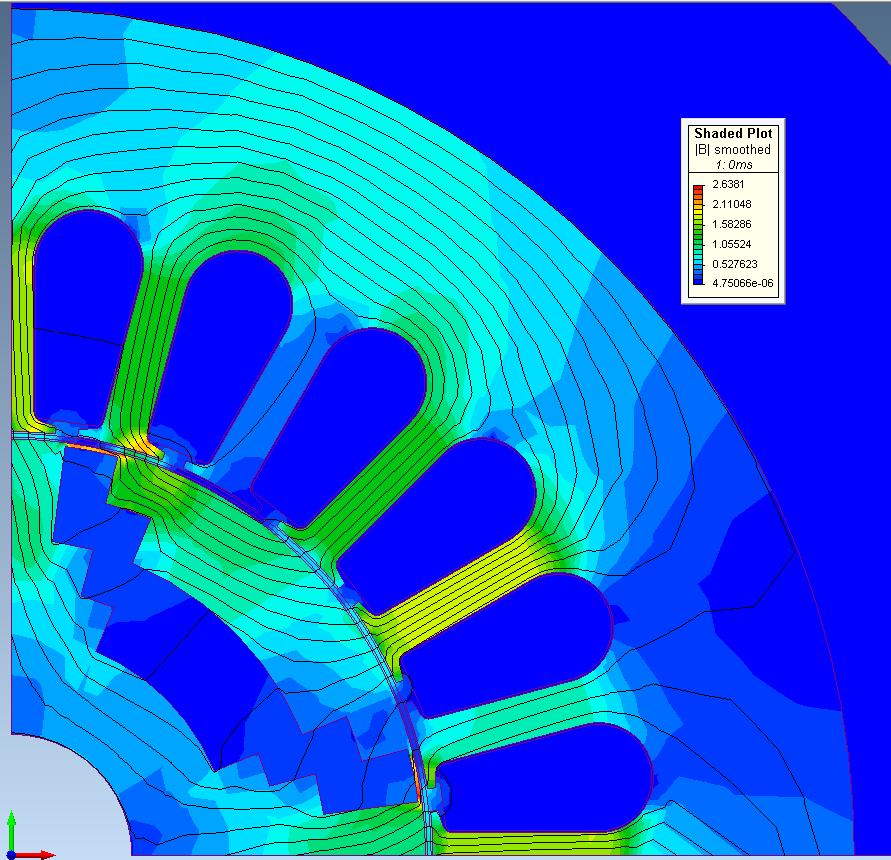
\includegraphics[width=\linewidth]{Figures/Ch_MDP/B_field_M19_IGTE2020.PNG}
  \caption{Magnetic $\left|B\right|$ field distribution}
  \label{fig:MDP_SynRM_Bfields}
\end{subfigure}
\caption{(a) Optimized geometry and the magnetic flux distribution for a discretized SynRM ($5 \times 5$ design space). SeqTO-\textit{v1} with GA.}
\label{fig:MDP_SynRM_GA_result}
\end{figure}

% Please add the following required packages to your document preamble:
% \usepackage{graphicx}
\begin{table}[h!]
\centering
%\resizebox{\textwidth}{!}{%
\begin{tabular}{|c|c|c|c|c|}
\hline
\textbf{\begin{tabular}[c]{@{}c@{}}Environment \\ Type\end{tabular}} & \textbf{\begin{tabular}[c]{@{}c@{}}Design Variables\\ (m)\end{tabular}} & \textbf{\begin{tabular}[c]{@{}c@{}}Population \\ Size\end{tabular}} & \textbf{\begin{tabular}[c]{@{}c@{}}Stall \\ Generation\end{tabular}} & \textbf{\begin{tabular}[c]{@{}c@{}}Average \\ Torque \end{tabular}} \\ \hline
$5 \times 5$ (Non-linear)                                                     & 25                                                                      & 25\|50                                                               & 25                                                                   & 3.40 N-m                                                               \\ \hline
\end{tabular}%
%}
\caption{TO results for SynRM using GA on the rotor structure; based on \textit{SeqTO-v1}}
\label{tab:MDP_synrm_ga}
\end{table}

\subsection{SynRM - TD-Learning results}

For the combination of geometric and excitation parameters mentioned in Table \ref{tab:MDP_synRM_fixed_parameters}, a sequence-based controller is also employed on a 5x5 discretized space. The discretized design space (Figure \ref{subfig:MDP_SynRM_dual_blank2}) is filled with M-19 26 Ga material and the controller is responsible for introducing air (barrier material). The optimal topology of the rotor is shown in Figure \ref{fig:MDP_SynRM_geometry_TD}. With an average torque of $3.40$ N-m, the resultant geometry, shown in Figure \ref{fig:MDP_SynRM_geometry_TD}, achieves a significant improvement in the average torque as compared to the torque ($2.5$ N-m) of the conventional design. The average torque ($T_{avg}$) is obtained through transient 2D Finite Element simulation \parencite{Magnet}.

% Please add the following required packages to your document preamble:
% \usepackage{graphicx}
\begin{table}[h!]
\centering
%\resizebox{\textwidth}{!}{%
\begin{tabular}{|c|c|c|c|c|}
\hline
\textbf{Environment Type} & \textbf{\begin{tabular}[c]{@{}c@{}}Episode \\ Length\end{tabular}} & \textbf{\begin{tabular}[c]{@{}c@{}}Learning\\ Rate\end{tabular}} & \textbf{\begin{tabular}[c]{@{}c@{}}Reward\\ Function\end{tabular}} & \textbf{\begin{tabular}[c]{@{}c@{}}Average\\ Torque \end{tabular}} \\ \hline
5 $\times$ 5 (Non-linear)          & 25                                                                 & 0.8                                                              &                                    $\nabla T$                                & 3.40 N-m                                                                        \\ \hline
\end{tabular}%
%}
\caption{SynRM results using TD-learning with SeqTO-\textit{v1}.}
\label{tab:MDP_synrm_td}
\end{table}
 
\begin{figure}[h!]
\centering
\begin{subfigure}{.5\textwidth}
  \centering
  \includegraphics[width=\linewidth]{Figures/Ch_MDP/SynRM_dual_optimal_M19_3.3476Nm.png}
  \caption{Optimal geometry}
  \label{fig:MDP_SynRM_geometry_TD}
\end{subfigure}%
\begin{subfigure}{.5\textwidth}
  \centering
  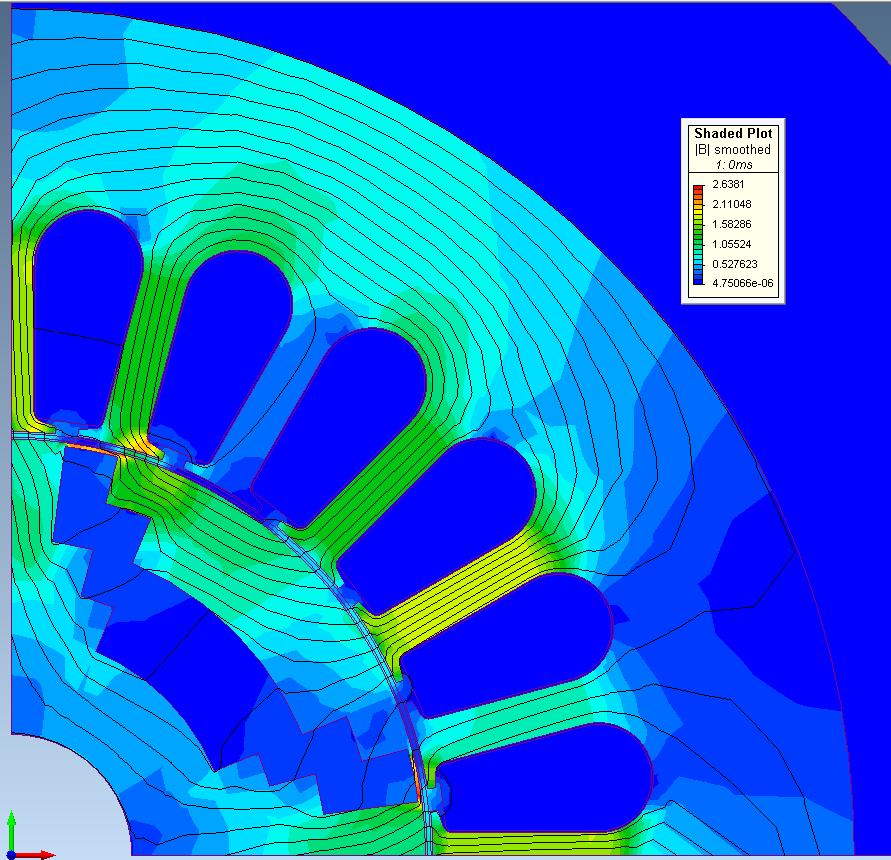
\includegraphics[width=\linewidth]{Figures/Ch_MDP/B_field_M19_IGTE2020.PNG}
  \caption{Magnetic $\left|B\right|$ field distribution}
  \label{fig:MDP_SynRM_Bfields_TD}
\end{subfigure}
\caption{(a) Optimized geometry and the magnetic flux distribution for a discretized SynRM ($5 \times 5$ design space). SeqTO-\textit{v1} with TD-learning.}
\label{fig:MDP_SynRM_GA_result}
\end{figure}

\section{Comparison between ON/OFF \& SeqTO-\textit{v1}}
\label{section:MDP_comparison_OnOFF_SeqTO}

Apart from the advantage of enforcing the connectivity of material, which directly results in manufacturable designs, Sequence-based TO is also efficient in terms of the total number of function calls during the optimization procedure, as seen during experimentation. This improvement can be verified by the data in Table \ref{tab:MDP_results}, where the number of function calls made using Sequence-based TO is reduced by a factor of around 4 - 5, as compared to ON/OFF TO methodology for the same design problem.

% Please add the following required packages to your document preamble:
% \usepackage{booktabs}
% \usepackage{graphicx}
\begin{table}[h!]
\centering
\resizebox{\textwidth}{!}{%
\begin{tabular}{@{}l|cc|cc|cc@{}}
\toprule
& \multicolumn{2}{c|}{\begin{tabular}[c]{@{}c@{}}GA\\ ON/OFF\end{tabular}} 
& \multicolumn{2}{c|}{\begin{tabular}[c]{@{}c@{}}GA\\ SeqTO-\textit{v1}\end{tabular}} 
& \multicolumn{2}{c}{\begin{tabular}[c]{@{}c@{}}TD \\ SeqTO-\textit{v1}\end{tabular}} 
\\ \midrule
Scenario 
& {\begin{tabular}[c]{@{}c@{}}Optimal\\ value\end{tabular}} 
& {\begin{tabular}[c]{@{}c@{}}FE\\ Simulations\end{tabular}}
& {\begin{tabular}[c]{@{}c@{}}Optimal\\ value\end{tabular}}       
& {\begin{tabular}[c]{@{}c@{}}FE\\ Simulations\end{tabular}}     
& {\begin{tabular}[c]{@{}c@{}}Optimal\\ value\end{tabular}}     
& {\begin{tabular}[c]{@{}c@{}}FE\\ Simulations\end{tabular}}                     \\
\hline                                
3 $\times$ 3 C-core Linear &           70 N                       &             20000                        &          70 N                        &                4500                     &                  70 N                &                3750                      \\
3 $\times$ 3 C-core (NL) &           51 N                       &             45000                        &          51 N                        &                7200                     &                  51 N                &                6000                      \\ 
SynRM                     &                3.4  N-m                 &             12000                        &          3.4 N-m                        &                   3000                  &                 3.4 N-m                  &                  2800                    \\ \bottomrule
\end{tabular}%
}
\caption{Comparison of On/Off TO with Seq based TO using GA \& TD-learning}
\label{tab:MDP_results}
\end{table}

This computational efficiency can be attributed to the reduced dimensionality of possible candidate designs to explore with SeqTO, due to the inherent requirement of enforced connectivity. This limitation imposed by SeqTO helps avoid the evaluation/generation of candidate designs with floating or isolated material. Further, in a comparison between the GA and TD-based learning when applied on SeqTO, it is found experimentally that TD based learning requires about 15-20\% fewer FE evaluations for generating the same optimal designs for linear and non-linear C-core design problem (using a controller of size  $3 \times 3$). However, the number of FE calls for both GA and TD show a smaller difference (around 6.5\%) for TO of the SynRM, which can be explained due to the relatively smaller design space of SynRM of $5 \times 5 = 25$ as compared to that of a C-core ($288$ elements in C-core design space). The computation cost presented in Table \ref{tab:MDP_results} is calculated by the average performance over many independent runs to make a scientific comparison. The random seed is the only difference between runs of these algorithms. 

\begin{figure}[h!]
    \centering
    \begin{subfigure}{0.45\textwidth}
        \centering
        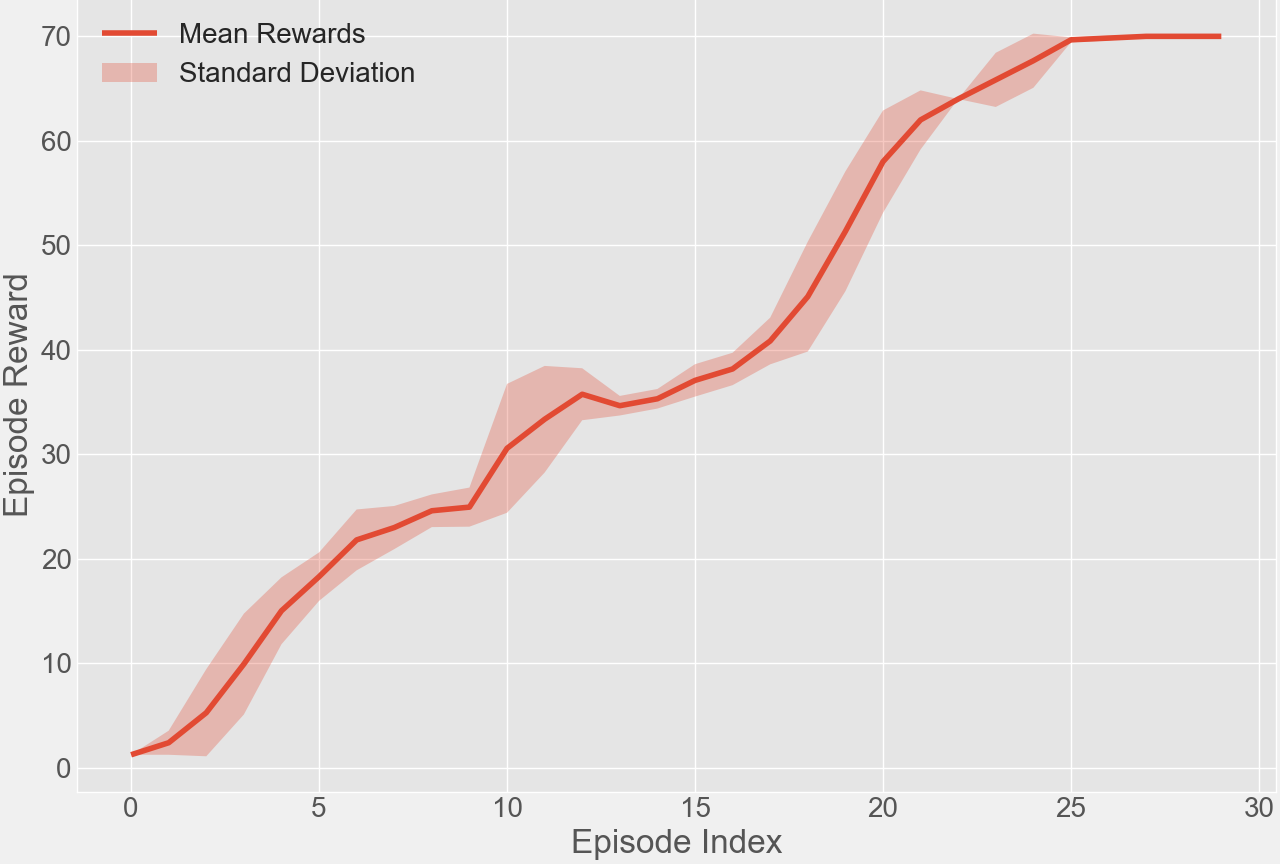
\includegraphics[width=\linewidth]{Figures/Ch_MDP/c_core_linear_training2.png}
        \caption{C-core (Linear material) $3 \times 3$ controller size}
        \label{fig:c_core_linear_training_rewards}  
    \end{subfigure}
    \begin{subfigure}{0.45\textwidth}
        \centering
        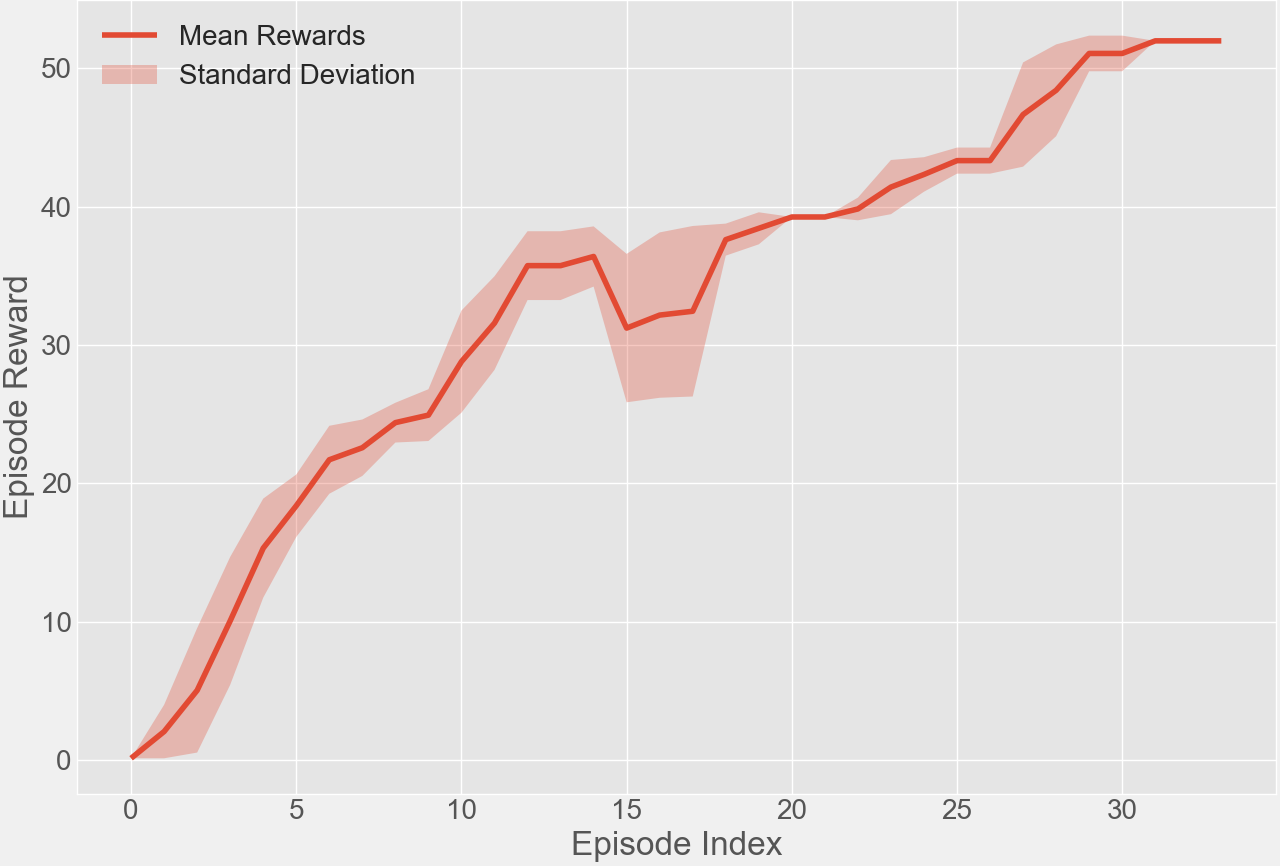
\includegraphics[width=\linewidth]{Figures/Ch_MDP/c_core_non_linear_training2.png}
        \caption{C-core (Non-linear material) $3 \times 3$ controller size}
        \label{fig:c_core_nonlinear_training_rewards}  
    \end{subfigure}
    \begin{subfigure}{0.65\textwidth}
        \centering
        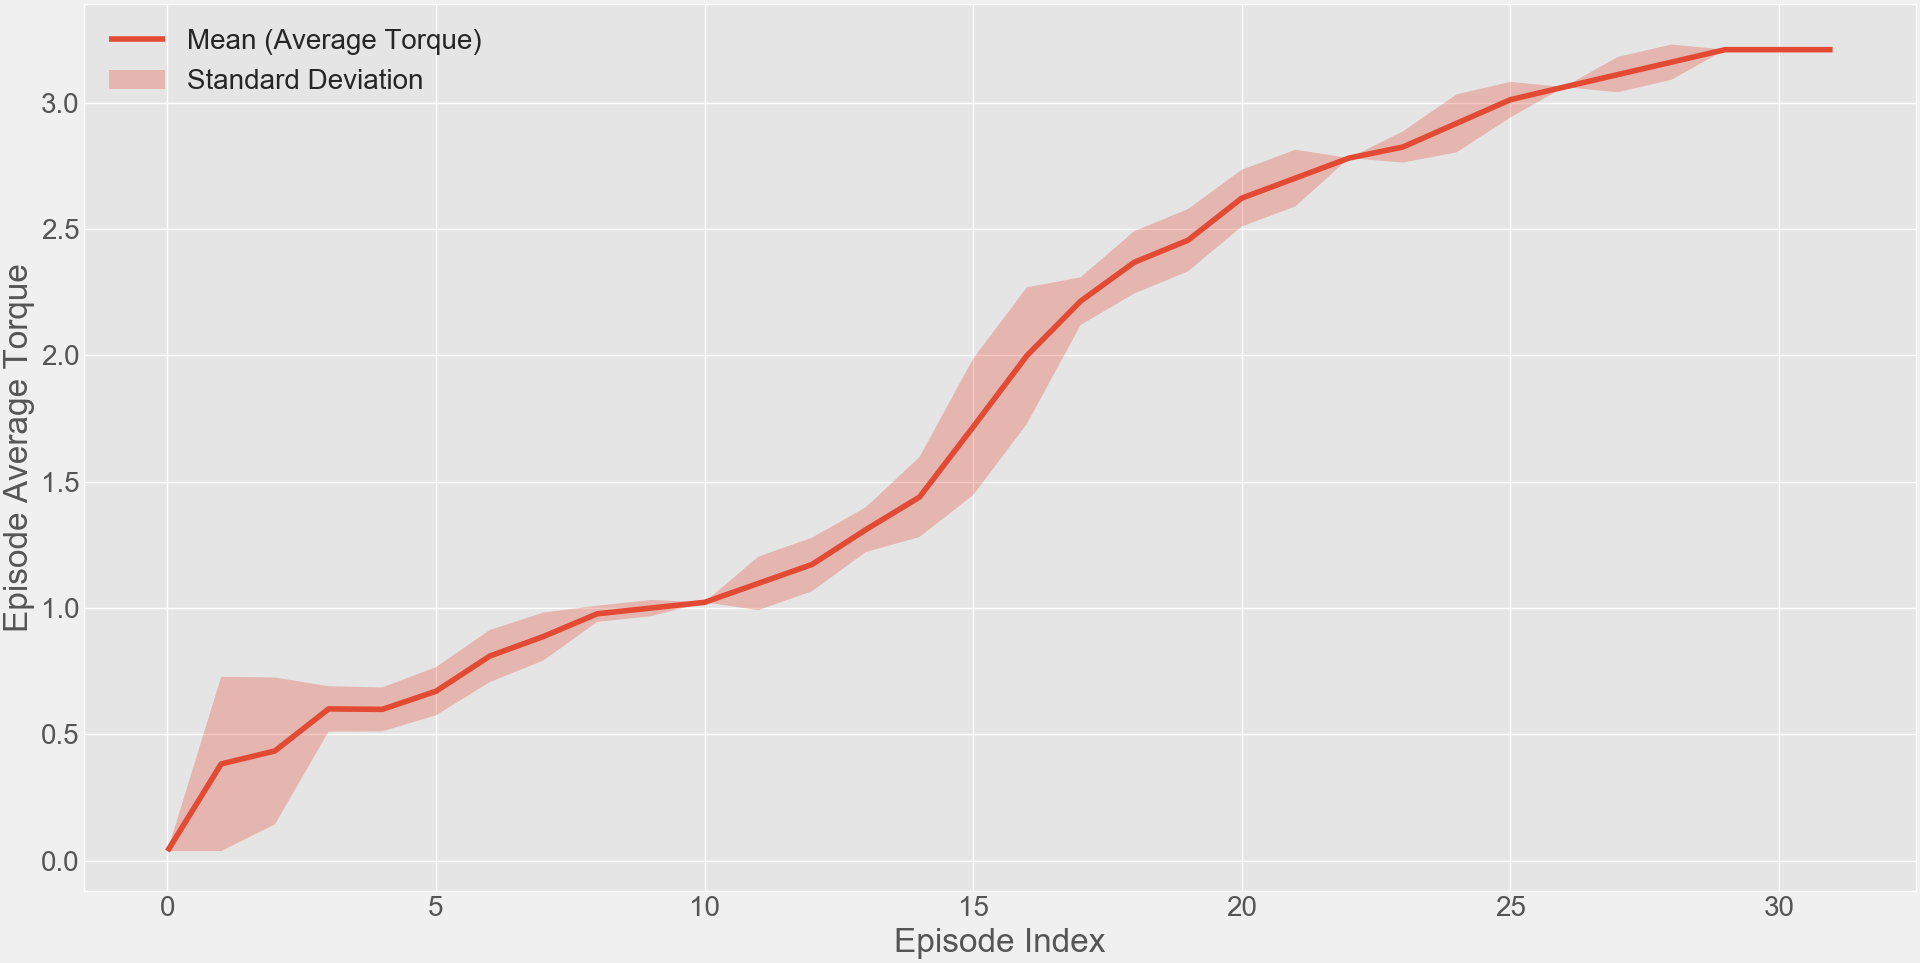
\includegraphics[width=\linewidth]{Figures/Ch_MDP/SynRM_training.png}
        \caption{SynRM $5 \times 5$ design space}
        \label{fig:synRM_training_rewards}  
    \end{subfigure}
    \caption{Training Rewards vs Episodes}
    \label{fig:MDP_raining_results}
\end{figure}

The transitional progress of learning with the TD-algorithm is shown in Figure \ref{fig:MDP_raining_results} (a), (b), (c) for C-core (using linear and non-linear material) and SynRM respectively. The graph is plotted by testing the TD algorithm on a fresh episode after a regular interval and no training is performed during this test episode. The solid line in the curves is the running average of the past few test runs and the standard deviation of the local averaging. As can be seen, the TD algorithm continues the learning process until the running average converges to a fixed value and the variance diminishes to a very low value.

Although a FE solver \parencite{Magnet} is used for all electromagnetic analyses in this study, this is neither a necessary requirement nor a limitation associated with any of the optimization algorithm discussed in this work. Any EM solver able to evaluate the desired performance criteria for the problem geometry and has an interface with the optimization algorithm should be sufficient enough for this work.

\section{Conclusion}

The feasibility of a sequence-based (SeqTO-\textit{v1}) controller for Topology Optimization is proved on several geometries of varying complexity. Furthermore, the working applicability of SeqTO with vastly different algorithms such as GA and QL as potential optimization processes is also shown. The structures obtained using the sequence-based controller were free from any island/stray material. The ability of SeqTO to generate such compact designs is useful for multiple engineering domains apart from electromagnetics, as the methodology can be easily imported to other design problems. The ability to work with significantly different algorithms such as GA and TD-learning and resulting in optimal solution proves the efficacy of sequence-based design optimization.
In TD-learning, the additional information gained through observing the actions taken by the controller along with the effect on the performance, at different steps of an episode, introduces interpretability in the whole design process. This additional information can be useful for designers to understand the impact of different components in the design. Exploiting this knowledge can result in further hand-tuned designs and offer more flexibility to a designer.

Moreover, breaking the whole geometry into a series of sub-components lays the path to apply more generalizable algorithms such as Deep Reinforcement Learning models, using Deep Neural Networks (DNN). Leveraging the complexity of a DNN to handle problems of high dimensionality has additional advantages, such as the ability to transfer knowledge learned from one environment to another, conditioned on having a similar sub-structure and relatable performance criteria. These possibilities will be explored in Chapter \ref{chapter:5_RL}. 



